\documentclass[a4paper,twoside,DIV15,BCOR12mm,11pt]{scrbook}


\usepackage{Analysis}

\makeindex

\begin{document}

\pagenumbering{arabic}
\setcounter{page}{1}

%!TEX root = FunkAnalysis.tex

\maketitle
%!TEX root = FunkAnalysis.tex

%\chapter*{Vorwort}
%Dieses Skript wurde im Wintersemester 2015/2016
%von Martin Belica geschrieben. Es beinhaltet die Mitschriften aus
%der Vorlesung von Prof.~Dr.~Weis sowie die Mitschriften einiger
%Übungen.


\section*{Einleitung}

Die Funktionalanalysis liefert den begrifflichen Rahmen sowie allgemeine Methoden, die in weiten Teilen der modernen Analysis verwendet werden. Zum Beispiel ist es möglich Integral- und Differentialgleichungen als lineare Gleichungen in einem geeigneten unendlichdimensionalen Vektorraum (wie z.B. einem Raum stetiger oder integrierbarer Funktionen) aufzufassen. Will man nun auf diese unendlichdimensionalen Gleichungen Ideen der linearen Algebra anwenden, so treten Konvergenz- und Kompaktheitsprobleme auf, die wir in dieser Vorlesung behandeln wollen. Zu den Themen gehören:

  \begin{itemize}
     \item Beschränkte und abgeschlossene Operatoren auf normierten Räumen
     \item Stetigkeit und Kompaktheit auf metrischen Räumen
     \item Geometrie und Operatorentheorie in Hilberträumen
     \item Der Satz von Hahn-Banach und Dualität von Banachräumen    
  \end{itemize}
  
Die allgemeinen Aussagen werden durch konkrete Beispiele von Räumen und Operatoren der Analysis illustriert.

\section*{Erforderliche Vorkenntnisse}
Analysis I-III, Lineare Algebra I-II

\tableofcontents 
\newpage

\markleft{Funktionalanalysis}
%!TEX root = Funktionalanalysis - Vorlesung.tex
\chapter*{Einf{\"u}hrung} \addcontentsline{toc}{chapter}{Einf{\"u}hrung}
  

\setcounter{section}{1}


\subsection*{R{\"a}ume}


Sei $X$ ein Vektorraum, $dim X < \infty $ und sei $x = (x_{1},\dotsc,x_{n})^{T} \in \MdR^{n}$
\begin{align*}
	\|x\|_{2}~ & \coloneqq \left(\sum_{k = 1}^{n} \|x_{i}^{2}\| \right)^{\frac{1}{2}}\\
	\|x\|_{\infty} & \coloneqq \smash{\displaystyle\max_{i = 1}^{n}}  \|x_{i}\|	
\end{align*}	

Diese Normen sind äquivalent, denn:
$\| x \|_{\infty} \leq \| x \|_{2} \leq n^{\frac{1}{2}} \| x \|_{\infty}$ 

\begin{satz}[Bolzano-Weierstra{\ss}] \index{Bolzano-Weierstrass} \label{satz:1.1-BolzanoWeierstrass}
Sei $A \subset \MdR^{n}$ beschränkt. Dann hat jede Folge $(x_{n})_{n \in \MdN} \subset A$ eine konvergente Teilfolge.
\end{satz}


\begin{beispiel}
	Betrachte $X = C[0, 1] = \{ f \colon [0, 1] \rightarrow \MdR: f \text{ stetig auf } [0, 1] \} $ mit $\| f \|_{\infty} \coloneqq  \smash{\displaystyle\max_{t \in [0, 1]}}  \| f(t) \|$. \\ 
	Sei weiter $f_{n} \colon t \rightarrow t^{n}$, damit gilt $\| f_{n} \|_{\infty} \leq 1 \quad \forall n \in \MdN$.	
	\begin{figure}[H]	
		\begin{center}					
			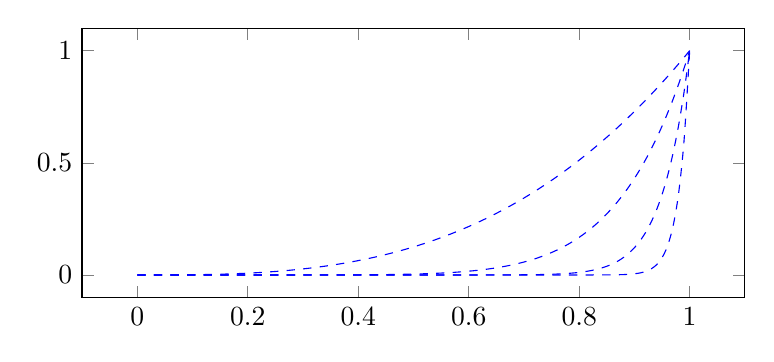
\begin{tikzpicture}
				\begin{axis}[domain=0:1, samples=101, height=5cm, width=10cm]
					\addplot [color=blue, thin, dashed, smooth] { ( x^(3) ) };
					\addplot [color=blue, thin, dashed, smooth] { ( x^(8) ) };
					\addplot [color=blue, thin, dashed, smooth] { ( x^(20) ) };
					\addplot [color=blue, thin, dashed, smooth] { ( x^(50) ) };
				\end{axis}
			\end{tikzpicture}
			\caption{$f_{n}$ für $n = 3, 8, 20$ und $50$}
		\end{center}
	\end{figure}					
	Die Folge $(f_{n})_{n \geq 1}$ besitzt damit aber in $X$ keine konvergente Teilfolge, da die Grenzfunktion
		\[ f = \begin{cases} 0 & x \in [0, 1) \\ 1 & x = 1 \end{cases} \]
	nicht in $X$ liegt. $ \Rightarrow $ \hyperref[satz:1.1-BolzanoWeierstrass]{Satz von Bolzano-Weierstra{\ss}} gilt im unendlich dimensionalen i.A. nicht!
\end{beispiel}


\subsection*{Operatoren}


Sei $N = dim X, M = dim Y$ und seien $(e_n)$ bzw. $(f_n)$ Basen von $X$ bzw. $Y$. 	\\
Sei $T \colon X \rightarrow Y$ gegeben durch: \\
\[ \begin{xy} \xymatrix{
	X \ar[r]^T	\ar[d]_{ \alpha_{n} \rightarrow \sum \alpha_{n} e_{n} }  &   Y \ar[d]^{ \beta_{n} \rightarrow \sum \beta_{n} f_{n} }  \\
      	\MdR^{N} 	\ar[r]^A    				&   \MdR^{n}  				
} \end{xy} \]
wobei $x = \sum \alpha_{n} e_{n},\hspace{0.2cm} Tx = \sum \beta_n f_n, \hspace{0.2cm} \beta_m = \sum_{n = 1}^{N} a_{mn} \alpha_{n}. $ \\ \\
Daraus folgt:
\begin{itemize}
	\item $T$ ist stetig
	\item X = Y \gdw T injektiv \gdw T surjektiv (Dimensionsformel) \\
	(Die Gleichung $Tx = y$ ist eindeutig lösbar $\gdw$ Gleichung hat für alle $y \in Y$ eine Lösung.)
	\item Falls A selbstadjungiert ist, d.h. $A = A^{*}$, gibt es eine Basis aus Eigenvektoren $(e_{n})$ von $A$, d.h. $ T( \sum_{n=1}^{N} \alpha_{n} e_{n} ) = \sum_{n=1}^{N} \lambda_{n} \alpha_{n} e_{n}$, wobei $\lambda_{n}$ Eigenwerte sind, d.h. 
		\[ A =
			\begin{pmatrix}
				\diagentry{\lambda_{1}}\\
				&\diagentry{\xddots}\\
				&&\diagentry{\lambda_{n}}\\
			\end{pmatrix} \]
\end{itemize}


\begin{beispiel}
$X = C^{1}[0, 1] = \{ f \colon [0, 1] \rightarrow \MdR: f \text{ stetig auf } [0, 1] \}$ \\
$T f = f', T \colon X \rightarrow C[0, 1] \text{ stetig.} $ (Aber: $T: C[0, 1] \rightarrow C[0, 1]$, hier ist $T$ nicht definiert.) \\

$T$ ist nicht stetig bzgl. $\| \cdot \|_{\infty}$-Norm, da:
\[ f_{n}(t) = \frac{1}{\sqrt{n}}e^{int}, \hspace{0.5cm}  \text{dann: } \|f_{n}\| \rightarrow 0 \text{ für } t \rightarrow \infty \]	
\[ T f_{n}(t) = i \sqrt{n} e^{int}, \hspace{0.5cm} \text{mit: } \| T f_{n} \|_{\infty} \rightarrow \infty, \text{ für } n \rightarrow \infty \]
\end{beispiel}


\begin{beispiel}
$X = L_{2} = \{ (a_{n}): \left( \sum_{n \geq 1}^{\infty} \| a_{n} \| \right)^{\frac{1}{2}} < \infty \}$	\\
$T ( a_{1}, a_{2}, a_{3}, ...) = ( 0, a_{1}, a_{2}, a_{3}, ...)$ \\

$T$ ist injektiv, aber nicht surjektiv
\end{beispiel}


\subsection*{Anwendungen}


\begin{enumerate}
	\item \begriff{Fredholm'sche Integralgleichungen}: \index{Fredholm'sche Integralgleichung} Sei $X = C[0, 1]$ und $k: [0, 1] \times [0, 1] \rightarrow \MdR$ stetig. Definiere $Tf(t) \coloneqq \int_{0}^{1} k(t, s) f(s) ds$ \textit{(Analogie zum endlich dim. als 'Verallg. der Matrixmultiplikation' mit} $T(f_{j})(i) = \sum_{j = 1}^{n} a_{ij}f_{j}$\textit{)}. \\
 	$T$ ist in diesem Fall linear und stetig und es gilt die Fredholm'sche Alternative:
	\[ \lambda \in \MdR \setminus \{0\}: (\lambda Id - T)(f) = y, \hspace{0.25cm} f,g \in C[0, 1] \]
	und eine Lösung existiert genau dann, wenn diese eindeutig ist. \\
	\item \begriff{Dirichletproblem}: \index{Dirichletproblem} Sei $\Omega \subset \MdR^n$ ein offenes, beschränktes Gebiet mit glattem Rand und sei $g \colon \partial \Omega \rightarrow \MdR$ stetig. Gesucht ist ein $f \in C(\bar \Omega) \cap  C^(\Omega)$, so dass $\nabla f = \sum_{i = 1}^{n} \frac{\partial^{2} f}{\partial x_{i}^2} = 0$ in $\Omega$ und $f|_{\partial \Omega}= g$. \\
	Beispiel: Durch Wärmeverteilung auf dem Rand auf die Wärmeverteilung im Inneren schlie{\ss}en. \\ \\
	Lösung: Dirichletintegral $J(u) = \int_{\Omega} (\nabla u )^{2} dx$, wobei $ u \in M = \{ v \in C^{1}(\bar \Omega) | \hspace{0.25cm} v|_{\partial \Omega} = g \}$ \\
	Sei $v_{0}$ das absolute Minimum von $J$, d.h. $J(v_{0}) = \inf \{ J(w): w \in M \}$ . Ist $v \in C^{1}(\bar \Omega)$ mit $v = 0$ in einer Umgebung von $\partial U$. $\epsilon \rightarrow J(u_{0} + \epsilon v)$:
	\[ \frac{d}{d\epsilon} J(u_{0} + \epsilon v) = \int_{\Omega} \frac{d}{d\epsilon} (\nabla u_{0} + \epsilon \nabla v)^{2} dx = 2 \int_{\Omega} (\nabla u_{0} + \epsilon \nabla v)(\nabla v) dx|_{\epsilon = 0} = 2 \int_\Omega (\nabla u_{0}) (\nabla v) dx \]
	Mit $0 \geq J(u_{0} + \epsilon v)- J(u_{0}) \geq 0: \hspace{0.25cm} \int (\nabla u_{0})(\nabla v) dx \overset{\text{P.I.}}{{=}} - \int (\nabla u_{0})v dx = 0$
	\[ \Rightarrow \nabla u_{0} = 0 \text{, au{\ss}erdem } u_{0 }|_{\partial \Omega} = g \text{ (s.o.)} \]
	Im Allgemeinen existiert das, das absolute Minimum $u_{0} \in J$ aber nicht. \\
	Ausweg: $X = \{ f \in L^{2}(\Omega), f' \in L^{2}(\Omega) \} \supset \{f \in C(\bar \Omega), f' \in C(\bar \Omega) \} $
	In diesem Raum $X$ (Sobolevräume) gibt es ein Minimum $u_{0}$ von $J$.
	\item  \begriff{Sturm-Liouville Problem}: \index{Sturm-Liouville Problem} Gegeben $X = C^{2}([0, 1]), Tu = (pu')' + qu$, mit $q \in C[0, 1], p \in C^{1}[0, 1]$, finde bei gegebenen $f \in C[0, 1]$ ein $u \in X$ mit $Tu = f, v(0) = 0, v'(1) = 0$. \\ \\
	Sei $Y = \{ f \in L^{2}[0, 1], f' \in L^{2}[0, 1] \}$ ein Hilbertraum und $(e_{n})$ ein Orthonormalbasis. Wäre:$\| e_{n} \|_{2} = 1, \int e_{n}(x) e_{m}(x) dx = 0$ für $m \neq m$: 
		\[ f \in Y: f = \sum_{n = 1}^{\infty} \alpha_{n} e_{n} \text{ mit } \| f \|^2 = \sum | \alpha_{n} |^2 \]
	Die $(e_{n})$ sind au{\ss}erdem Eigenvektoren des Operatoren $T$, d.h. $Te_{n} = \lambda_{n} e_{n}$ \\
	\[ Ty = f \Rightarrow \int Ty(x) e_{n}(x) dx = \int f(x) e_{n}(x) dx, y = \sum_{n = 1}^{\infty} \alpha_{n} e_{n} \]
	Gesucht sind die Koeffizienten $\alpha_{n}$
	\begin{align*}
		\int f(x) e_{n}(x) dx & = \sum_{m} \lambda_{m} \alpha_{m} \int T e_{n}(x) e_{m}(x) dx \\
							  & =  \lambda_{n} \alpha_{n} \int e_{n}(x) e_{n}(x) dx
	\end{align*}
	\[ \gdw \alpha_{n} = \frac{1}{\lambda_n} \int f(x) e_{n}(x) dx \]
\end{enumerate}



\newpage
%!TEX root = Funktionalanalysis - Vorlesung.tex

\chapter*{Lineare Operatoren auf Banachräumen} \addcontentsline{toc}{chapter}{Lineare Operatoren auf Banachräumen} \setcounter{section}{1}



\section{Normierte R{\"a}ume}



\begin{definition}
	Sei $X$ ein Vektorraum über $\MdK \in\{ \MdR, \MdC \}$. \\
	Eine Abbildung  $\| \cdot \| \colon X \rightarrow \MdR_{+}$ hei{\ss}t eine \begriff{Norm}, wenn
		\begin{description}
			\item[$\hspace{0.5cm} (N1) \hspace{0.1cm} $] $\| x \| \geq 0, \quad \| x \| = 0 \gdw x = 0 $
			\item[$\hspace{0.5cm} (N2) \hspace{0.1cm} $] $\| \lambda x \| = | \lambda \| x \| $
			\item[$\hspace{0.5cm} (N3) \hspace{0.1cm} $] $\| x + y \| \leq \| x \| + \| y \| $
	\end{description}	
\end{definition}


\begin{bemerkung}
	Falls $ \| \cdot \| $ all die oben genannten Eigenschaften erfüllt au{\ss}er $ \| x \| = 0 \Rightarrow x = 0 $, dann hei{\ss}t $ \| \cdot \| $ Halbnorm.
\end{bemerkung}


\begin{vereinbarung}
Die Menge $ U_{X} = \{ x \in X:  \|x \| \leq 1 \}$ hei{\ss}t \begriff{Einheitskugel}. \\
Eine Folge $(x_{n})$ des normierten Raums $X$ \begriff{konvergiert} gegen ein $ x \in X $, falls  $\| x_{n} - x \| \xrightarrow[n \rightarrow \infty]{} 0. $	
\end{vereinbarung}


\begin{bemerkung}
Für zwei Elemente $x, y \in (X, \| \cdot \|)$ in normierten Räumen gilt auch die \begriff{umgekehrte Dreiecksungleichung} $( | \| x \| + \| y \| | \leq \| x + y \|)$
\end{bemerkung}


\begin{beispiel}
Sei $ X = \MdK^{n}, \hspace{0.25cm} x = ( x_{1}, \dotsc, x_{n}), \hspace{0.25cm} x_{i} \in \MdK$ 
\begin{align*}
	\| x \|_{p} & = \left( \sum_{j = 1}^{n} |x_{j}^{p}| \right)^{\frac{1}{p}}, \quad 1 \leq p < \infty \text{ } (p = 2: \text{ Euklidische Norm}) \index{Euklidische Norm} \\
	\| x \|_{\infty} & = \hspace{0.3cm} \sup_{j = 1}^{n} |x_{j}|	
\end{align*}

Beh.: $\| \cdot \| $ ist Norm auf $\MdK^n$ für $1 \leq p \leq \infty$

$\| x + y \|_{\infty} = sup_{j = 1}^{k} |x_{j} + y_{j}| \leq \|x\|_{\infty} + \|y\|_{\infty} $
Für $p \in (1, \infty), p \neq 2:$ siehe Übungsaufgabe (Fall $p = 2$ läuft über Cauchy-Schwarz)

Beachte: $\|x\|_{\infty} \leq  \|x\|_{p} \leq n^{\frac{1}{p}} \|x\|_{\infty} \leq n \| x \|_{\infty}$
\end{beispiel}


\begin{definition}
	Zwei Normen $\| \cdot \|_{1}, \| \cdot \|_{2}$ hei{\ss}en \begriff{äquivalent} auf $X$, falls es $0 < m, M < \infty$ gibt, so dass für alle $ x \in X$ gilt:
	\[ m \| x \|_{2} \leq \| x \|_{1} \leq M \| x \|_{2} \]
\end{definition}
 
 
\begin{satz} 
	Auf einem endlich dimensionalen Vektorraum sind alle Normen äquivalent.
\end{satz}

\begin{beweis}
	Wähle eine algebraische Basis $(e_{1}, \dotsc, e_{n})$ von X, wobei $ n = dim X < \infty$. \\
	Definiere $ \vertiii{x} = \left(\sum_{i = 1}^{n} |x_{i}|^2\right)^{\frac{1}{2}}$, wobei $x = \sum_{i = 1}^{n} x_{i} e_{i}$ \\
	
	z. z. die gegeben Norm $\vertiii{ \cdot }$ ist äquivalent zu $\| \cdot \|$. \\ \\
	Beweis: \\
	In der einen Richtung betrachte: 
	\begin{align*}
		\| x \| = \left\| \sum_{i = 1}^{n} x_{i} e_{i} \right\| & \leq \sum_{i = 1}^{n} |x_{i}| \|  e_{i} \| \\ 
													& \leq \underbrace{ \left( \sum_{i = 1}^{n} |x_{i}|^{2} \right)^\frac{1}{2} }_{=: \vertiii{ x }} \underbrace{ \left( \sum_{i = 1}^{n} \| e_{i} \|^{2} \right)^\frac{1}{2} }_{=: \nu}
	\end{align*}
	
	Für die Umkehrung benutze die Funktion $J \colon \MdK^{n} \rightarrow X, \hspace{0.1cm} J(x_{1}, \dotsc, x_{n}) = \sum_{i = 1}^{n} x_{i} e_{i} $ \\
	\begin{align*}
 	 \text{Die Abbildung } y & \in \MdK^{n}  \rightarrow \| Jy \| \text{ ist stetig, denn} \\
 	 	 \vertiii{ Jy } = \| y \|_{\MdK^{n}} & = \left( \sum_{i = 1}^{n} |y_{i}|^{2} \right)^{\frac{1}{2}}, y = (y_{1}, \dotsc, y_{n}) \\
 	 	 \text{und } \left| \| Jy \| - \| Jz \| \right| & \leq | \| Jy - Jz \| = | \| J(y - z) \| \\
 	 	 & \leq \nu \vertiii{ J (y - z) } \\
 	 	 & = M \| y - z \|_{\MdK^{n}} \\
 	 \end{align*}
 Daraus folgt die Stetigkeit von $ y \rightarrow \| Jy \| \in \MdR $ \\ \\
	Sei $S = \{y \in \MdK^{n}: \| y \|_{\MdK^n} = 1 \}$. Dann ist $S$ abgeschlossen und beschränkt.
	Die Abbildung $N \colon y \in S \rightarrow \| Jy \| > 0$ ist wie in (*) gezeigt stetig. Nach Analysis II nimmt $N$ sein Minimum in einem Punkt $y_{0} \in S$ an. Setze
		\begin{align*}
			m = \inf\{\| x \| : \vertiii{ x } = 1\} & = \inf \{ \| Jy \|: y \in S \} \\
												& = \| J y_{0} \| > 0 \\ \\
			\text{Also } m \leq \| \frac{x}{ \vertiii{ x } } \| =  \frac{ \| x \| }{ \vertiii{ x } }  &\Rightarrow \vertiii{ x } \leq m \| x \|.
		\end{align*}
\end{beweis}


\begin{prop}
	Für zwei Normen $\| \cdot \|_{1}, \| \cdot \|_{2}$ auf $X$ sind äquivalent:
	\begin{enumerate}[label=\alph*\upshape)]
		\item $\| \cdot \|_{1}, \| \cdot \|_{2}$ sind äquivalent
		\item Für alle $(x_{n}) \subset X$, $x \in X$ gilt $\| x_{n} - x \|_{1} \rightarrow 0 \gdw \| x_{n} - x \|_{2} \rightarrow 0 $
		\item Für alle $(x_{n}) \subset X$ gilt $\| x_{n} |_{1} \rightarrow 0 \gdw \| x_{n} \|_{2} \rightarrow 0 $
		\item Es gibt Konstanten $0 < m$, $M < \infty$, so dass $m U_{(X, \| \cdot \|_{1})} \leq U_{(X, \| \cdot \|_{2})} \leq M U_{(X, \| \cdot \|_{1})}$
	\end{enumerate}
	\begin{beweis}
		\begin{description}
			\item[] $a) \Rightarrow b) \Rightarrow c)$ folgt direkt durch die Definition von äquivalenten Normen. 
  			\item[] $c) \Rightarrow d)$ Annahme: Es existiert kein $M$ mit $U_{(X, \| \cdot \|_{2})} \subset M U_{(X, \| \cdot \|_{1})}$. \\
  				Dann gibt es eine Folge $x_{n} \in U_{(X, \| \cdot \|_{2})}$ mit $\| x_{n} \|_{1} \geq n^{2}$ \\
  				Setze $y_{n} =  \frac{1}{n} x_{n}$. Dann gilt $\| y_{n} \|_{1} \rightarrow 0$ und $\| y_{n} \|_{2} \rightarrow \infty$. \\
  				Widerspruch zu $c)$.
  			 \item[] $d) \Rightarrow a)$ Gegeben ist $U_{(X, \| \cdot \|_{2})} \subset M U_{(X, \| \cdot \|_{1})}$ \\
  			 Das ist äquivalent zu $\| x \|_{2} \leq M \| x \|_{1}$ \\
  			 Analog folgt aus $m U_{(X, \| \cdot \|_{1})} \subset U_{(X, \| \cdot \|_{2})}$ dann $m \| x \|_{1} \leq \| x \|_{2}$. \\
  			 Also $m \| x \|_{1} \leq \| x \|_{2} \leq M \| x \|_{1}$ 
		\end{description}
	\end{beweis}
\end{prop}


\begin{vereinbarung}
	Sei $\MdF = \{ (x_{n}) \in \MdK^{\MdN}: x_{i} = 0 \text{ bis auf endlich viele } n \in \MdN \} $ der \begriff{Folgenraum} \\
	und $e_{j} = (0, \dotsc, 0, 1, 0, \dotsc, 0) $ der Einheitsvektor, wobei die $1$ an j-ter Stelle steht.
\end{vereinbarung}


\begin{beispiel} \index{l$^{p}$-Raum} \index{l$^{\infty}$-Raum} \index{c$_{0}$-Raum}
	\begin{itemize}
		\item $\ell^{p} = \{ x = (x_{n}) \in \MdK^{\MdN}: \|x\|_{p} = \left( \sum_{n = 1}^{\infty} | x_{n} |^{p}\right)^{\frac{1}{p}} < \infty \}$
		\item $\ell^{\infty} = \{ x = (x_{n}) \in \MdK^{\MdN  }: \|x\|_{\infty} = \sup_{n \in \MdN} |x_{n}| < \infty \}$
		\item $c_{0} = \{ x = (x_{n}) \in \ell^{\infty}: \lim_{n \rightarrow \infty} |x_{n}| = 0 \}$
	\end{itemize}
	Gültigkeit der Dreiecksungleichung beweist man ähnlich wie bei $(\MdK^{n}, \| \cdot \|_{p})$.
\end{beispiel}


\begin{lemma}
	\begriff{Minkowskii-Ungleichung}: $\left( \sum_{i=1}^{\infty} |x_{i} + y_{i}|^p\right)^{\frac{1}{p}} \leq\left( \sum_{i=1}^{\infty} |x_{i}|^p\right)^{\frac{1}{p}} \left( \sum_{i=1}^{\infty} |y_{i}|^p\right)^{\frac{1}{p}} $	\\
	\begriff{Hölder-Ungleichung}: mit $\frac{1}{p} + \frac{1}{p'} = 1 \text{ gilt } \sum_{i=1}^{\infty} |x_{i}| |y_{i}| \leq \left( \sum_{i=1}^{\infty} |x_{i}|^{p} \right)^{\frac{1}{p}} \left( \sum_{i=1}^{\infty} |y_{i}|^{p'} \right)^{\frac{1}{p'}} $	\\	
\end{lemma}


\begin{bemerkung}
	Im unendlich dimensionalen Fall sind die Normen $\| \cdot \|_{p}$ auf $\MdF$ nicht äquivalent.
	\begin{beweis}
		Sei $p > q$, setze 
		\[ X_{n} \coloneqq \sum_{j = 2^{n} + 1}^{2^{n + 1}} j^{-\frac{1}{p}}e_{j}, \hspace{0.5cm} e_{j} = ( \delta_{ij} )_{u \in \MdN} \]
		Damit gilt $x_{n} \in \MdF$ und weiter
		\[ \| x_{n} \|_{p} = \left( \sum_{j = 2^{n}}^{2^{n + 1}} \frac{1}{j} \right)^{\frac{1}{p}} \simeq \left( ln(2) \right)^{\frac{1}{p}} \]
		aber $\| x_{n} \|_{q} \rightarrow \infty$, also sind $\| \cdot \|_{p}, \| \cdot \|_{q}$ keine äquivalente Normen.
	\end{beweis}	
\end{bemerkung}


\begin{beispiel}
	\begin{enumerate}[label=\alph*\upshape)]
		\item Raum der stetigen Funktionen \index{Raum der stetigen Funktionen} \\
		$\Omega \subset \MdR^{n}, \hspace{0.25cm} C(\Omega) = \{ f \colon \Omega \rightarrow \MdR \text{ | } f \text{ stetig} \}$, \hspace{0.25cm} $\| f \|_{\infty} = \sup_{u \in \Omega} |f(u)|$\\
		$\Rightarrow \| f - f_{n} \|_{\infty} \rightarrow 0$ bedeutet gleichmä{\ss}ige Konvergenz von $f_{n}$ gegen $f$ auf $\Omega$.
		\item Raum der differenzierbaren Funktionen \index{Raum der differenzierbaren Funktionen} \\
		$\Omega \subset \MdR^{n}$ offen, $f \colon \Omega \rightarrow \MdR, \hspace{0.25cm} \alpha = (\alpha_{1}, \dotsc, \alpha_{m}) \in \MdN_{0}^{m}$ \\
		$D^{\alpha}f(x) = \frac{ \delta^{ | \alpha | } }{ \delta x_{1}^{ \alpha_{1} } \dotsc \delta x_{n}^{ \alpha_{n} } } f(x), \text{ wobei } | \alpha | = \alpha_{1} + \dotsc + \alpha_{n} $ \\ 
	\end{enumerate}
\end{beispiel}


\begin{definition}
	Wir nennen $C_{b}^{m}(\Omega) = \{ f \colon \Omega \rightarrow \MdR | D^{\alpha}f \text{ sind stetig in } \Omega, \text{ beschränkt auf } \Omega \text{ für alle } \alpha \in \MdN^{n}, |\alpha| \leq m \}$ den \begriff{Raum der beschränkten, m-fach stetig differenzierbaren Funktionen}.  \\
	Auf $C_{b}^{m}$ definieren wir die Norm: $\| f \|_{C_{b}^{m}} = \sum_{|\alpha| \leq m} \| D^{\alpha}f \|_{\infty}$
\end{definition}


\begin{bemerkung}
	Auf $C_{b}^{m} [0, 1]$ ist eine äquivalente Norm zu  $\| f \|_{C_{b}^{m}}$ gegeben durch
	\begin{align*}
		\| f \|_{0} & = \sum_{i = 0}^{m - 1} |f^{(i)}(0)| + \| f^{(m)} \|_{\infty} \\
		\text{Denn } f^{(i)}(t) = f^{(i)}(0) + \int_{0}^{t} & f^{(i + 1)}(s) ds \text{ und damit } \| f^{(i)}\|_{\infty} \leq | f^{(i)}(0) | + \| f^{(i + 1)}\|_{\infty}	
	\end{align*}
\end{bemerkung}


\begin{beispiel}
	$X = C(\bar\Omega), \Omega \subset \MdR^{n}$ offen, beschränkt. \\
	Definiere $\| f \|_{L^{p}} = \left( \int_{\Omega} |f(u)|^{p} du \right)^{\frac{1}{p}}$ und betrachte $f_{k}(t) = t^k, t \in [0, 1]$, dann gilt:
 	\[ \| f \|_{L^{p}} = \left( \frac{1}{kp + 1} \right)^{\frac{1}{p}} \xrightarrow[k \rightarrow \infty]{} 0, \hspace{0.25cm} p < \infty \]
\end{beispiel}


\begin{definition}[\begriff{Quotientenräume}] \label{def:2.15-Quotientenraeume}
	Sei $(X, \| \cdot \|)$ ein normierter Raum. $M \subset X$ sei abgeschlossener, linearer Unterraum. \[ (\text{abgeschlossen: d.h. für alle } (x_{n}) \in M, \| x_{n} - x \| \rightarrow 0 \Rightarrow x \in M) \]

	Definiere $\hat X = X / M, \hspace{0.25cm} \hat x \in X/M: \hspace{0.25cm} \hat x = \{ y \in X: y - x \in M \} = x + M$ \\
	Dabei gilt unter anderem $\hat x_{1} + \hat x_{2} = \widehat{x_{1} + x_{2}}$ und $\lambda \hat x_{1} = \widehat{\lambda x_{1}}$; $\hat X$ bildet somit einen Vektorraum. \\
	Definieren wir eine Norm für die Äquivalenzklassen mittels $\| \hat x \|_{\hat X} : = \inf \{ \| x - y \|_{X}: y \in M \} =: d(x, Y)$

	Behauptung: $(\hat X, \| \cdot \|_{\hat X})$ ein normierter Raum. \\
	Beweis: Sei $\hat x \in \hat X$ beliebig mit $\| \hat x \|_{\hat X} = 0$ \\
	dann existiert ein $y_{n} \in \hat X \text{ mit } \| y_{n} \| \rightarrow 0$ und $x - y_{n} \in M$
	\[ \Rightarrow x \in M, \hat x = 0 \]
	Zu $\epsilon > 0$ wähle für $\hat x_{1}, \hat x_{2} \in \hat X, y_{1}, y_{2} \in M$ mit
	\[ \| \hat x_{i} \| \geq \| x_{i} - y_{i} \| - \epsilon \] 
	Damit folgt:
	\begin{align*}
		\| \widehat{x + y} \| & \leq \| x_{1} + x_{2} - y_{1} - y_{2} \| \\
						  & \leq \| x_{1} - y_{1} \| + \| x_{2} - y_{2} \| \\
						  & \leq \| \hat x_{1} \| + \| \hat x_{2} \| + 2 \epsilon
	\end{align*}
\end{definition}


\begin{bemerkung}
	Ist $\| \cdot \|$ nur eine Halbnorm auf $X$, so ist $M = \{ x: \| x \| = 0 \}$ ein abgeschlossener, linearer Teilraum von $X$ und der Quotientenraum $(\hat X, \| \cdot \|_{\hat X})$ ist ein normierter Raum.
\end{bemerkung}
\newcommand{\rquot}[2]{\raisebox{0.5ex}{$#1$}\!/\!\raisebox{-0.5ex}{$#2$}}
\begin{beispiel}
	\begin{itemize}
		\item Hölderstetige Funktionen \index{Hölderstetige Funktionen} \\
			Wenn $h_{\alpha}(f) = \sup_{u,v \in \MdR, u \neq v} \frac{\| f(u) - f(v)\|}{|u - v|^{\alpha}} < \infty \hspace{0.25cm} \left( \alpha \in (0, 1] \right)$, dann nennt man $f$ hölderstetig.
			\[ C^{\alpha}(\Omega) \coloneqq \{ f \colon \Omega \rightarrow \MdR: h_{\alpha}(f) < \infty \} \hspace{0.5cm} \Omega \subset \MdR^{n}, \hspace{0.25cm} \]
			Im Moment ist $h_{\alpha}( \cdot )$ eine Halbnorm. Unter der Voraussetzung $\Omega$ zusammenhängend gilt aber weiter:
			\[ h_{\alpha}(f) = 0 \gdw f \equiv c \text{ konstant} \]
			Wenn z.B. $M = \{ \1_\Omega \}$ und $V = C^{\alpha}/M$ ist oben genanntes sogar ein normierter Raum.
		\item Lebesgues-Integrierbare Funktionen \index{Lebesgue-Integrierbare Funktionen} \\
			Sei $\Omega \subset \MdR^{n}$ offen, $\cl^{p}(\Omega) = \{ f \colon \Omega \rightarrow \MdR : |f|^{p}$ ist Lesbesgue-integrierbar auf $\Omega$  \}.
			Wir definieren $\| f \|_{p} \coloneqq \left( \int_{\Omega} |f(x)|^{p} d\mu \right)^{\frac{1}{p}}$, wobei $\| \cdot \|_{p}$ hier eine Halbnorm bildet.
			\[ \| f \|_{p} = 0 \gdw  f(x) = 0 \text{ fast überall auf } \Omega \]
			Wähle $M = \{ f \colon \Omega \rightarrow \MdR: f = 0 \text{ fast überall auf } \Omega \}$. \\ \\
			Dann ist 
			\[ L^{p}(\Omega) \coloneqq \QR{ \cl^{p}(\Omega) }{ M } \text{ ein normierter Raum.} \]
	\end{itemize}
\end{beispiel}



\newpage
%!TEX root = Funktionalanalysis - Vorlesung.tex

\section{Beschr{\"a}nkte und lineare Operatoren}

\begin{definition}
	Eine Teilmenge V eines normieren Raums $(X, \| \cdot \|)$ hei{\ss}t \begriff{beschränkt}, falls 
	\[ c \coloneqq \sup_{x \in V} \| x \| < \infty, \text{ und damit auch } V \subset c U_{(X, \| \cdot \| )} . \]
\end{definition}


\begin{bemerkung}
	Eine konvergente Folge $(x_{n})	\in X, x_{n} \rightarrow x$ ist beschränkt, denn $x_{m} \in \{ y: \| x - y \| \leq 1 \}$ für fast alle $m$.
\end{bemerkung}


\begin{satz}
	Seien $X$, $Y$ normierte Räume. Für einen linearen Operator $S: X \rightarrow Y$ sind äquivalent:
	\begin{enumerate}[label=\alph*\upshape)]
		\item $T$ stetig, d.h. $x_{n} \rightarrow x$ impliziert $Tx_{n} \rightarrow Tx$
		\item $T$ stetig in 0
		\item $T(U_{(X, \| \cdot \|)})$ ist beschränkt in $Y$
		\item Es gibt ein $c < \infty$ mit $\| Tx \| \leq c \| x \|$
	\end{enumerate}	
\end{satz}

\begin{beweis}
	\begin{description}
		\item[] $a) \Rightarrow b)$ klar, ist ein Spezialfall.
		\item[] $b) \Rightarrow c)$ Wäre $c)$ falsch, dann gibt es ein $x_{n} \in U_{X}$ mit 
		\[ \| T x_{n} \| \geq \frac{1}{n^{2}} \]
		Setze $y_{n} = \frac{1}{n} x_{n}$, dann gilt
		\[
			\| y_{n} \| \leq \frac{1}{n} \| x_{n} \| \rightarrow 0, \\
			\| T y_{n} \| = n^{2} \| T(x_{n}) \| \geq \frac{n^2}{n} \rightarrow \infty 
		 \]
		 Widerspruch zur Voraussetzung.
		 \item[] $c) \Rightarrow d)$ Sei $T(U_{X}) \subset U_{Y}$ \\
		 Für $x \in X \setminus \{0\}, \frac{x}{\| x \|} \in U_{X}$ folgt:
		 \begin{align*}
		 	&T \left( \frac{x}{\| x \|} \right) \in c U_{Y} \\
		 	\Rightarrow \| T \left( \frac{x}{\| x \|} \right) \| & \leq c
		 	\Rightarrow \| T x \|_{Y} \leq c \| x \|_{X}			
		 \end{align*}
		 \item[] $d) \Rightarrow a)$ Für $x_{n} \rightarrow x$ in $X$ folgt:
		 \begin{align*}
		 	\| T x_{n} - T x \| & = \| T ( x_{n} - x ) \| \\
		 						& \leq c \| x_{n} - x \| \rightarrow 0
		 \end{align*} \[ \Rightarrow T x_{n} \rightarrow T x \text{ in } Y \]
	\end{description}
\end{beweis}
	
	
\begin{definition}
	Seien $X, Y$ normierte Räume. Mit $B(X, Y)$ bezeichnen wir den \begriff{Vektorraum der beschränkten, linearen Operatoren} $T: X \rightarrow Y$. Ist $ X = Y$ schreiben wir auch kurz $B(X) \coloneqq B(X, X)$. \\
	
	Für $T \in B(X, Y)$ setze
	\begin{align*}
		\| T \| & = \sup \{ \frac{\| Tx \|}{\| x \|}: x \in X \ {0} \} \\
				& = \sup \{ \| Tx \|: \| x \| \leq 1 \}
	\end{align*}
	Die Norm $\| T \|$ von $T$ ist die kleinste Konstante $c$, für welche die Gleichung $\| Tx \| \leq c \| x \|$ für alle $x \in X$ gilt.
\end{definition}


\begin{satz}
 	$(B(X, Y), \| \cdot \|)$ ist ebenfalls ein normierter Raum und für $X = Y$ gilt für $S, T \in B(X)$:
 	\[ \| S \cdotp T \| \leq \| S \| \| T \| \]
\end{satz}

\begin{beweis}
	$\| T \| \geq 0, \hspace{0.15cm} \| T \| = 0 \hspace{0.15cm} \Rightarrow \| Tx \| = 0$ für $\| x \| \leq 1 \hspace{0.15cm} \Rightarrow \hspace{0.15cm} Tx = 0 \hspace{0.15cm} \Rightarrow \hspace{0.15cm} T = 0$ \\
	\begin{align*}
		\| ( T + S )(x) \| = \| Tx + Sx \| &\leq \| Tx \| + \| Sx \| \\
										   &\leq \| T \| + \| S \|
	\end{align*}
	Nehme das Supremum über $\| x \| \leq 1$:
	\[ \| T + S \| \leq \| T \| + \| S \| \]
	\begin{align*}
		\| ( S \cdot T )(x) \| = \| S(Tx) \| & \leq \| S \| \| Tx \| \\
													 & \leq \| S \| \| T \| \| x \|
	\end{align*}
	\[ \Rightarrow \| S T \| \leq \| S \| \| T \| \]
\end{beweis}


\begin{beispiel}
	\begin{enumerate}[label=\alph*\upshape)]
		\item $Id x = x, \hspace{0.25cm} \|  Id \| = 1$
		\item Falls $dim X = n < \infty, Y$ normierter Raum, dann sind alle linearen Operatoren $T: X \rightarrow Y$ beschränkt.
		\begin{beweis}
			Wähle die Basis $e_{1}, \dotsc, e_{n}$ von $X$ \\
			Für $x = \sum_{i = 1}^{n} x_{i} e_{i}$ gilt:
			\begin{align*}
				\| Tx \| = \| \sum_{i = 1}^{n} x_{i} T e_{i} \| & \leq \sum_{i = 1}^{n} | x_{i} | \| T e_{i} \| \\
				& \leq \max_{i = 1}^{n} \| T e_{i} \|_{Y} \sum_{i = 1}^{n} |x_{i}| \\
				& \leq c \| x \|, \text{ da } \| x \| = \sum_{i = 1}^{n} |x_{i} |
			\end{align*}	
			Aber: Wenn $dim X = \infty, dim Y < \infty$ so gibt es viele unbeschränkte, lineare Operatoren von $X$ nach $Y$.
		\end{beweis}
		\item $X = C^{\infty}(0, 1), \| f \|_{\infty} = \sup_{u \in (0, 1)} |f(u)|$ \\
		$T:X \rightarrow X, Tf = f', f_{k}(t) = e^{i 2 \pi k t} \in X, Tf_{k}(t) = 2 \pi i k f_{k}(t)$ \\ 
		$ \| f_{k} \| = 1, \| Tf_{k} \| = 2 \pi k \rightarrow \infty $
		\item $\MdF = \{ (x_{n}) \in \MdR^{n}: x_{n} = 0 \text{ bis auf endlich viele } n \}$ \\
			\[ 
			  T: \MdF \rightarrow \MdR, \quad T( (x_{n}) ) = \sum_{n \in \MdN} n x_{n} \in \MdR, \quad
			 \| T e_{n} \| = n \rightarrow \infty
			\]
	\end{enumerate}	
\end{beispiel}


\begin{beispiel}[Integraloperator] \index{Integraloperator}
	$X = Y = C(\bar \Omega), \Omega \subset \MdR^{n}$ offen, beschränkt.
	Gegeben sei $k \in \bar \Omega \times \bar \Omega \rightarrow \MdR $
	
	Für $f \in C(\bar \Omega)$ setze: $Tf(u) = \int_{\Omega} k(u, v) f(v) dv$, \hspace{0.25cm}
	$\left( A( f_{j} ) \right)_{i} = \sum_{j = 1}^{n} a_{ij}f_{j}, A = (a_{ij})_{i,j = 1, \dotsc, n} )$ \\
	
	Dann ist $Tf \in C(\bar \Omega)$ (nach \hyperref[satz:x-SatzvonLebesgue]{Lebesguesschem Konvergenzsatz})
	\begin{align*}
		|T f(u)| & \leq \int_{\Omega} |k(u, v)| |f(u)| du \\
				 & \leq \int_{\Omega} |k(u, v)| du \sup_{u \in \Omega} | f(u) |
	\end{align*} 				 
	$\sup$ über $u \in \Omega$ liefert dann:
	\begin{align*}
		\| Tf \|_{\infty} \leq \sup_{u \in \Omega} \int |k(u,v)| dv \| f \|_{\infty} \\
		\Rightarrow \| T \| = \sup_{u \in \Omega} \int |k(u, v)| dv < \infty,
	\end{align*} 	
	Die Abbildung $u \in \bar \Omega \rightarrow \int |k(u, v)| dv \in \MdR$ ist stetig nach dem \hyperref[satz:x-SatzvonLebesgue]{Konvergenzsatz von Lebesgue}. \\
	\begin{beweis}
		$ "\ \leq "\ $ ist klar \\
		$ "\ \geq "\ $ Falls $ k(u, v) \geq 0$ dann ist $T \cdot \1 (u) = \int k(u, v) dv = \int |k(u, v)| dv$ \\
		\[ \| T \cdot \1 \| = \sup_{u \in \Omega} \int |k(u, v)| dv \leq \| T \| \text{, d.h. } \| \1 \| = 1 \]
		Skizze:
		\[ \sup \int | k(u, v) | dv \sim \int | k(u_{0}, v) | dv = \int k(u_{0}, v) g(v) dv \]
		mit $g(v) = sign(v) k(u_{0}, v), \hspace{0.25cm} g$ ist aber nicht stetig. \\
		Ggf. Approximation des Signums durch stetige Funktionen.
	\end{beweis}
\end{beispiel}


\begin{beispiel}[Kompositionsoperator] \index{Kompositionsoperator}
$\Omega \subset \MdR^{n}$ offen. 
\[ \sigma \colon \bar \Omega \rightarrow \bar \Omega \text{ stetig, für } f \in C(\bar \Omega): Tf(u) = f(\sigma(u)) \]
z.B.: $\sigma$ als Transposition der Elemente in $\Omega$
\[ \| Tf \|_{\infty} \leq \| f \|_{\infty}, \hspace{0.25cm} \| T \| = 1 \]
\end{beispiel}

\begin{beispiel}[Differentialoperatoren] \index{Differentialoperatoren}
	$\Omega \subset \MdR^n$ offen, $m \in \MdN$, $X = C^{m}(\bar \Omega), Y = C_{b}(\Omega),$
	\begin{align*}
		T:X \rightarrow Y, & \hspace{0.25cm} Tf(u) = \sum_{|\alpha| < m} a_{\alpha} D^{\alpha} f(u), u \in \MdR, a_{\alpha} \in C{\bar \Omega} \\
  		\text{damit } & \| Tf \|_{\infty} \leq \sum_{|\alpha| \leq m} \| a_{\alpha} \|_{\infty} \| D^{\alpha} f \|_{\infty} \leq c \|f\|_{\infty}	
  	\end{align*}
\end{beispiel}

\begin{beispiel}[Matrizenmultiplikation] \index{Matrizenmultiplikation}
	Für $p \in [1, \infty]$ und $T \in B(\ell^{p})$ setzen wir 
	\[ e_{l} \coloneqq (0, \dotsc, 0, 1, 0, \dotsc), \hspace{0.25cm} l \in \MdN, \hspace{0.25cm} \text{ wobei die 1 an l-ter Stelle steht.} \]
	und $a_{kl} = (T e_{l})_{k}$, sowie $A = (a_{kl})_{k,l \in \MdN}$
	\[ \Rightarrow (Tx)_{k} = (\sum_{l = 1}^{\infty} x_{l} T e_{l})_{k} = \sum_{ l = 1}^{\infty} a_{kl}k_{l}, \hspace{0.25cm} k \in \MdN \quad \Rightarrow \quad T x = A x \text{ (unendliches Matrixprodukt)} \]
	\begin{enumerate}[label=\alph*\upshape)]
		\item Die Hille-Tamarkin-Bedingung (nur hinreichend) \\
			Sei $p \in (1, \infty)$ und $\frac{1}{p} + \frac{1}{q} = 1$. Setze
			\[ c \coloneqq \left( \sum_{k \geq 1} \left( \sum_{l \geq 1} |a_{kl}|^{q} \right)^{\frac{p}{q}} \right)^{\frac{1}{p}} < \infty \]
			so definiert $T$ einen Operator $T \in B(\ell^{p})$ mit $\| T \| \leq c$ 
		\begin{beweis}
			\begin{enumerate}
				\item Wohldefiniertheit: (und Beschränktheit)  \\
					Für $x \in \ell^{p}$ folgt
					\begin{align*}
						\| Tx \|_{\ell^{p}}^{p} &= \sum_{k \geq 1} | (Tx)_{k} |^{p} \\
									 	 &= \sum_{k \geq 1} | \sum_{l \geq 1} |a_{kl} x_{l} |^{p} \\
										 &\leq \sum_{k \geq 1} \left( \sum_{l \geq 1} |a_{kl}|^{q} \right)^{\frac{p}{q}} \left( \sum_{l \geq 1} |x_{l}|^{p} \right)^{\frac{p}{q}} \\
										 &= c^{p} \|x\|_{\ell^{p}}^{p} < \infty
					\end{align*}
				\item Linearität \\
					Wegen $c < \infty$ ist $\left( \sum_{l} |a_{kl}|^{q} \right)^{\frac{1}{q}} < \infty, \hspace{0.1cm} \forall k \in \MdN$ \\
					Für $x \in \ell^{p}$ konvergiert die Reihe nach Hölder. Damit ist $T$ offensichtlich linear.
			\end{enumerate}
		\end{beweis}
	\item Der Fall $\ell^{1}$: \\
		Es ist $T \in B(\ell^{1})$ genau dann, wenn 
		\[ c_{1} \coloneqq \sup_{l} \sum_{k} | a_{kl} | < \infty \]
		und in diesem Fall ist $\| T \| = c_{1}$.
		\begin{beweis}
			"\ $\Rightarrow$ "\  Sei $T \in B(\ell^{1})$. Dann gilt für $l \in \MdN$
			\begin{align*}
				\sum_{k} | a_{kl} | &= \sum_{k} |(Te_{l})_{k}| \\
								  	&= \| T e_{l} \|_{\ell^{1}}  \\
								  	& \leq \| T \| \| e_{l} \|_{\ell^1} = \| T \| < \infty 
			\end{align*}
			"\ $\Leftarrow$ "\  folgt genau wie in a) mit Hölder. Au{\ss}erdem gilt $\| T \| \leq c_{1}$			
		\end{beweis}
	\item Der Fall $\ell^{\infty}$: \\
		Es ist $T \in B(\ell^{\infty})$ genau dann, wenn
		\[ c_{\infty} \coloneqq \sup_{k} \sum_{l} |a_{kl}| < \infty \]
		und in diesem Fall ist $\| T \| = c_{\infty}$
		\begin{beweis}
			"\ $\Rightarrow$ "\  Sei $T \in B(\ell^{\infty})$.  Für $k \in \MdN$ setze dann $x^{(k)} = \begin{cases} \frac{|a_{kl}|}{a_{kl}} & a_{kl} \neq 0 \\ 0 & a_{kl} = 0 \end{cases}$ \\
			dann ist $x^{(k)} \in \ell^{\infty}$ mit $\| x^{(k)} \|_{\ell^{\infty}} = 1$ und weiter
			\begin{align*}
				\sum_{l} |a_{kl}| & = | \sum_{l = 1}^{\infty} a_{nl} x_{l}^{(k)} | \\
								  & = | ( T x^{(k)} )_{k} | \\
								  & \leq \| T x^{(k)} \|_{\infty} \\
								  & \leq \| T \| \| x^{(k)} \|_{\ell^{\infty}} = \| T \|
			\end{align*}			
			\[ \Rightarrow c_{\infty} \leq \| T \| \]
			"\ $\Leftarrow$ "\ folgt genau wie in a) mit Hölder. Au{\ss}erdem gilt $\| T \| \leq c_{\infty}$ 
		\end{beweis}
	\item Interpolation \\
		Ist $T \in B(\ell^{1}) \cap B(\ell^{\infty})$, dann ist $T \in B(\ell^{p})$ für alle $p \in (1, \infty)$ mit $\| T \| \leq c_{1}^{\frac{1}{p}} c_{\infty}^{\frac{1}{q}}$, wobei $\frac{1}{p} + \frac{1}{q} = 1$
		\begin{beweis}
		 Für $x \in \ell^{p}$ setzen wir $y_{k} \coloneqq |(T x)_{k}|^{p - 1}, \hspace{0.25cm} k \in \MdN$ \\
		 \[ \Rightarrow \| y \|_{\ell^{q}} = \left( \sum_{k \geq 1} \left| \left( Tx \right)_{k} \right|^{\underbrace{q(p-1)}_{= p}}  \right)^\frac{1}{q} = \| Tx \|_{\ell^{p}}^{p - 1} \]	
		 Damit folgt
		 \begin{align*}
		 	\| Tx \|_{\ell^{p}}^{p} & = \sum_{k \geq 1 } y_{k} | (Tx)_{k} | \leq \sum_{k \geq 1} \sum_{l \geq 1} y_{k} |a_{kl}| |x_{l}| \\
		 	& = \sum_{k \geq 1} \sum_{l \geq 1} |a_{kl}|^{\frac{1}{p}} |a_{kl}|^{\frac{1}{q}} |y_{k}| |x_{l}| \\
		 	& \leq \left( \sum_{k \geq 1} \sum_{l \geq 1} |a_{kl}| |y_{k}|^{q} \right)^{\frac{1}{q}} \left( \sum_{k \geq 1} \sum_{l \geq 1} |a_{kl}| |x_{l}|^p \right)^{\frac{1}{p}} \\
		 	& \leq c_{\infty}^{\frac{1}{q}} \| y \|_{\ell^{q}} c_{1}^{\frac{1}{p}} \| x \|_{\ell^{p}} \\
		 	& =  c_{\infty}^{\frac{1}{q}} c_{1}^{\frac{1}{p}}  \| x \|_{\ell^{p}} \| Tx \|_{\ell^{p}}^{p - 1} 
		 \end{align*}
		 \[ \Rightarrow \| Tx \|_{\ell^{p}} \leq c_{1}^{\frac{1}{p}} c_{\infty}^{\frac{1}{q}} \| x \|_{\ell^{p}} \text{ und } \| T\| \leq c_{1}^{\frac{1}{p}} c_{\infty}^{\frac{1}{q}} \]
		\end{beweis}
 \end{enumerate}
\end{beispiel}

\begin{definition}
	Seien $X, Y$ normierte Vektorräume und $T: X \rightarrow Y$ linear.
	\begin{enumerate}[label=\alph*\upshape)]

		\item $T$ hei{\ss}t \begriff{Isometrie}, falls $ \| Tx \|_{Y} = \| x \|_{X} \hspace{0.25cm} \forall x \in X $
		\item $T$ hei{\ss}t \begriff{stetige Einbettung}, falls $T$ stetig und injektiv ist
		\item $T$ hei{\ss}t \begriff{isomorphe Einbettung}, falls $T$ injektiv ist und ein $c > 0$ existiert mit
			\[ \frac{1}{c} \| x \|_{X} \leq \| Tx \|_{Y} \leq c \| x \|_{x} \]
			In diesem Fall identifizieren wir oft $X$ mit dem Bild von $T$ in $Y$, $X \cong T(X) \subset Y$ 
		\item $T$ hei{\ss}t \begriff{Isomorphismus}, falls $T$ bijektiv und stetig ist und $T^{-1}: Y \rightarrow X$ ebenfalls stetig ist. 
			\[ \text{d.h. falls } \exists c > 0: \frac{1}{c} \| x \|_{X} \leq \| T x \|_{Y} \leq c \| x \|_{X} \]
			\[ \text{(daraus folgt dann auch für }T^{-1}: Y \rightarrow X \text{ aus der ersten Ungleichung } \]
			\[ \| T^{-1}y \|_{X} \leq c \| T (T^{-1}y) \|_{Y} = c \| y \|_{Y}, \text{d.h. } T^{-1} \text{ ist stetig.)}\]
			In diesem Fall Identifizieren wir $X \cong Y$ und sagen $X$ und $Y$ sind isomorph (da $X, Y$ normierte Vektorräume sind, fordern wir im Gegensatz zur Linearen Algebra, dass $T, T^{-1}$ zusätzlich stetig sind).
	\end{enumerate}
\end{definition}


\begin{beispiel}
	\begin{enumerate}[label=\alph*\upshape)]
		\item Seien $(X, \| \cdot \|_{1})$ und $(X, \| \cdot \|_{2})$ normierte Vektorräume. Dann gilt
			\[ \| \cdot \|_{1} \sim \| \cdot \|_{2} \gdw I: (X, \| \cdot \|_{1}) \rightarrow (X, \| \cdot \|_{2}), Ix = x \text{ ist isomorph} \]
		\item $I: c_{0} \hookrightarrow \ell^{\infty}, I x = x$ ist isometrische Einbettung
	\end{enumerate}
\end{beispiel}


\begin{definition}	
	Sei $X$ ein normierter Vektorraum. Der Raum
 		\[ X' = B(X, \MdK) \]	
 	hei{\ss}t \begriff{Dualraum} von $X$ oder Raum der linearen Funktionalen.
\end{definition}

\begin{beispiel}
	Sei $X = \ell^{p}$ für $p \in (1, \infty)$ und $\frac{1}{p} + \frac{1}{q} = 1$ \\
	Die Abbildung
	\[ \Phi_{p} \colon \ell^{p} \rightarrow (\ell^{p})', \hspace{0.25cm} [\Phi_{p}(x)](y) = \sum_{n = 1}^{\infty} x_{n} y_{n}, \hspace{0.25cm} x \in \ell^{p}, y \in \ell^{q}  \]
	Ist ein isometrischer Isomorphismus, d.h.  $(\ell^{p})' \cong \ell^{q}, \hspace{0.25cm}$ (insbesondere $(\ell^{2})' \cong \ell^{2}$)
	
	\begin{beweis}
		Nach Hölder konvergiert die Reihe $[\Phi_{p}(x)](y)$ absolut mit 
		\[ | [\Phi_{p}(x)](y) | \leq \sum_{n} |x_{n} y_{n}| \leq \| x \|_{\ell^{q}} \| y \|_{\ell^{p}} \]
		Da $\Phi_{p}(x)$ linear in $Y$ ist, folgt $\Phi_{p}(x) \in (\ell^{p})'$ mit
		\[ \| \Phi_{p}(x) \|_{(\ell^{p})'} \leq \| x \|_{\ell^{q}} \]
		Es bleibt zu zeigen, dass $ \| \Phi_{p}(x) \|_{(\ell^{p})'} \geq \| x \|_{\ell^{q}} $ und $\Phi_{p}$ surjektiv ist.
		Sei $y' \in (\ell^{p})'$, dann setze $x_{n} \coloneqq y'(e_{n}), n \in \MdN$ und $x = (x_{n})_{n \geq 1}$.
		Setze au{\ss}erdem
		\[ z_{n} \coloneqq \begin{cases} \frac{|x_{n}|^{q}}{x_{n}} & x_{n} \neq 0 \\ 0 & x_{n} = 0 \end{cases}, \hspace{0.25cm} n \ \in \MdN \]
		Dann gilt für $N \in \MdN$
		\begin{align*}
			\sum_{n=1}^{N} |x_{n}|^{q} & = \sum_{n = 1}^{N} x_{n} z_{n} \\
			& = \sum_{n = 1}^{N} y'(e_{n}) z_{n} = y'\left(\sum_{n = 1}^{N} z_{n} e_{n} \right) \\
			& \leq \| y' \|_{(\ell^{p})'} \underbrace{ \|  \sum_{n = 1}^{N} z_{n} e_{n} \|_{\ell^{p}} }_{= \left( \sum_{n = 1}^{N} |x_{n}|^{(q - 1)p} \right)^{\frac{1}{p}}} \\
			& = \left( \sum_{n = 1}^{N} |x_{n}|^{q}\right)^{\frac{1}{p}}
		\end{align*}
		\[ \text{Also zusammen: } \left( \sum_{n = 1}^{N} |x_{n}|^{q} \right)^{1-\frac{1}{p}} \leq \| y \|_{(\ell^{p})'}, \text{ wobei } 1 - \frac{1}{p} = \frac{1}{q} \]
		\begin{align}
			\xRightarrow{N \rightarrow \infty} \| x \|_{\ell^{q}} \leq \| y' \|_{\ell^{\infty}} < \infty, \text{ d.h. } x \in \ell^{q} \label{eq:3.14-proof-ineqlqlinf}			
		\end{align} 
		Da für $y \in \ell^{p}$
		\[ \| y - \sum_{n = 1}^{N} y_{n} e_{n} \|_{\ell^{p}}^{p} = \sum_{n \geq N + 1} |y_{n}|^{p} \rightarrow 0 \text{ für } N \rightarrow \infty \]
		folgt
		\[ | y' (y) - \sum_{n = 1}^{N} y' ( y_{n} e_{n} ) | \leq \| y' \| \| y - \sum_{n = 1}^{N} y_{n} e_{n} \|_{\ell^{p}}  \rightarrow 0 \hspace{0.5cm} (N \rightarrow \infty) \]
		und damit \\
		\begin{align*}
			[ \Phi_{p} (x) ](y) & = \sum_{n = 1}^{\infty} x_{n} y_{n} \\
			& = \sum_{n = 1}^{\infty} y'(y_{n} e_{n}) \hspace{0.25cm} \\
			& = y'(y) \forall y \in \ell^{p} 		
		\end{align*}
		d.h. $ \Phi_{p}(x) = y'$ und damit $\Phi_{p}$ surjektiv.
		Au{\ss}erdem gilt nach \eqref{eq:3.14-proof-ineqlqlinf}
		\[ \| \Phi_{p}(x) \|_{(\ell^{p})'} \geq \| x \|_{\ell^{q}}, \]
		womit die Behauptung gezeigt ist.
	\end{beweis}
\end{beispiel}


\begin{bemerkung*}
	\begin{enumerate}[label=\alph*\upshape)]
		\item Analog zu obigem zeigt man $(\ell^{1})' \cong \ell^{\infty}$ und $(c_{0})' \cong \ell^{1}$
		\item Eine ähnliche Aussage gilt auch für $L^{p}$-Räume auf einem Ma{\ss}raum $(\Omega, \ca, \mu):$
			Hier gilt:
			\[ L^{p}(\Omega, \mu)' \cong L^{q}(\Omega, \mu) \]
			bezüglich der Dualität $[\Phi_{p}(f)](g) (= \langle f, g \rangle ) = \int_{\Omega} f(x) g(x) d\mu(x)$ wobei $p \in [1, \infty),$ $\frac{1}{p} + \frac{1}{q} = 1$
	\end{enumerate}	
\end{bemerkung*}


\begin{beispiel} \label{bsp:3.15}
	\begin{enumerate}[label=\alph*\upshape)]
		\item Sei $K \subset \MdR^{n}$ kompakt, $x \in K$. Dann definieren wir
			\[ \delta_{x}(f) \coloneqq f(x) \text{ für } f \in C(K) \]
			Wir versetzen $C(K)$ mit der Supremumsnorm. Dann gilt:
			\[ |\delta_{x}(f)| = | f(x) | \leq \| f \|_{\infty} \]
			und offensichtlich ist $\delta_{x}$ linear, d.h. $\delta_{x} \in ( C(K) )'$ mit $\| \delta_{x} \| \leq 1$.
		\item Sei $K \subset \MdR^{n}$ kompakt und $\mu$ ein endliches Ma{\ss} auf $\cb(K)$. Dann definieren wir 
			\[ \delta_{\mu}(f) = \int_{K} f(x) d\mu(x) \text{ für } f \in C(K) \]
			Dann gilt
			\[ | \delta_{\mu} (f) | \leq \mu(K) \| f \| _{\infty}. \]
			Da $\delta_{\mu}$ linear ist, gilt $\delta_{\mu}\in (C(K))'$ mit $\delta_{\mu} \leq \| \mu (K) \|$. In diesem Sinne sind Ma{\ss}e Elemente von $(C(K))'$
	\end{enumerate}	
\end{beispiel}


\begin{bemerkung}
	Man kann zeigen, dass $(C(K))' \cong M(K)$, wobei $M(K)$ die Menge der 'regulären' Borelma{\ss}e versehen mit der Variationsnorm ist. Die Dualität ist gegeben durch
	\[ (T \mu)(f) = \int_{K} f(x) d\mu(x) \]
\end{bemerkung}



\newpage
%!TEX root = Funktionalanalysis - Vorlesung.tex

\section{Metrische R{\"a}ume}

\begin{definition}
	\begin{enumerate}[label=\alph*\upshape)]
		\item Sei $M$ eine nichtleere Menge. Eine Abbildung $d \colon M \times M \rightarrow 	\MdR$ hei{\ss}t \begriff{Metrik} auf $M$, falls $\forall x, y, z \in M:$
			\begin{description}
				\item[$\hspace{0.5cm} (M1) \hspace{0.1cm} $] $d(x, y) \geq 0, \hspace{0.25cm} d(x, y) = 0 \gdw x = y $  (positive Definitheit)
				\item[$\hspace{0.5cm} (M2) \hspace{0.1cm} $] $d(x, y) = d(y, x)$  (Symmetrie)
				\item[$\hspace{0.5cm} (M3) \hspace{0.1cm} $] $d(x, z) \leq d(x, y) + d(y, z)$  (Dreiecksungleichung)
			\end{description}
			Das Tupel $(M, d)$ nennen wir dann einen metrischen Raum. 
		\item Eine Folge $(x_{n})_{n \geq 1} \subset M$ konvergiert gegen $x \in M$, falls
			\[ d(x_{n}, x) \rightarrow 0 \hspace{0.5cm} \text{für } n \rightarrow \infty \]	 
			Notation: $x = \lim_{n \rightarrow \infty} x_{n}$ (in $M$)
	\end{enumerate}
\end{definition}


\begin{bemerkung*}
	Der Grenzwert einer konvergenten Folge ist stets eindeutig, denn: \\
	Sei $(x_{n})_{n \geq  1} \subset M$ mit $\lim_{n \rightarrow \infty} x_{n} = x \in M$ und $\lim_{n \rightarrow \infty} x_{n} = y \in M$, dann folgt: 
	\begin{align*}
		d(x, y) & \leq d(x, x_{n}) + d(x_{n}, y) \\
				& \rightarrow 0 \text{ für } n \rightarrow \infty
	\end{align*}
	d.h. $d(x, y) = 0 \Rightarrow x = y$
\end{bemerkung*}


\begin{beispiel}
	\begin{enumerate}[label=\alph*\upshape)]
		\item Sei $X$ ein normierter Vektorraum und $M \subset X$ (nichtleere) Teilmenge. \\
		Dann definiert $d(x, y) \coloneqq \| x - y\|, \hspace{0.25cm} x, y \in M$ eine Metrik auf $M$ \\
		Ein Unterschied hier: Eine Norm setzt eine lineare Struktur auf $X$ voraus, eine Metrik macht auch Sinn auf nicht-linearen Teilmengen.
		\item \label{bsp:1-diskreteMetrik} Sei $M$ eine nichtleere Menge, dann definieren wir die \begriff{diskrete Metrik} auf $M$ durch
			\[ d(x, y) \coloneqq \begin{cases}1 &, x \neq y \\ 0 &, x = y\end{cases} \]
			Dann ist $(M, d)$ ein metrischer Raum und es gilt: 
				\[ x_{n} \rightarrow x \text{ in } M \gdw \exists N \in \MdN \text{ mit } x_{n} = x \hspace{0.25cm} \forall n \geq N \]
	\end{enumerate}	
\end{beispiel}


\begin{beispiel}  \label{bsp:4.3}
	\begin{enumerate}[label=\alph*\upshape)]	
		\item Sei $X$ ein Vektorraum und $p_{j}$ für $j \in \MdN$ Halbnormen auf $X$ mit der Eigenschaft, dass für jedes $x \in X \setminus \{ 0 \}$ ein $K \in \MdN$ existiert mit $p_{K} > 0$. Dann definiert
			\[ d(x, y) \coloneqq \sum_{j \geq 1} 2^{-j} \frac{p_{j}(x - y)}{1 + p_{j}(x -y)}, \hspace{0.5cm} x, y \in X \]
			eine Metrik auf $X$ mit
			\[ d(x_{n}, x) \rightarrow 0 \gdw p_{j}(x_{n} - x) \rightarrow 0 \hspace{0.25cm} (n \rightarrow  \infty) \hspace{0.25cm} \forall j \in \MdN \]
			Beweis siehe Übung
		\item Für $X = \MdK^{\MdN} = \{ (x_{n})_{n \geq 1}: x_{n} \in \MdK \}$ und $p_{j}(x) \coloneqq |x_{j}|, j \in \MdN$ definiert also
			\[ d(x, y) = \sum_{j = 1}^{\infty} 2^{-j} \frac{|x_{j} - y_{j}|}{1 + |x_{j} - y_{j}|} \text{ gerade die komponentenweise Konvergenz auf } X \]
		\item In $\ell^{\infty}$ entspricht die Konvergenz bezüglich $\| \cdot \|_{\ell^{\infty}}$ gerade der gleichmä{\ss}igen Konvergenz der Folge $x_{n} \coloneqq (x_{n, i})_{(i \in \MdN)}$ gegen $x \coloneqq (x_{i})_{(i \in \MdN)}$
			\[ \| x_{n} - x \|_{\ell^{\infty}} = \sup_{i \in \MdN} | x_{n, i} - x_{i} | \rightarrow 0 \hspace{0.5cm} (n \rightarrow \infty) \]
		\item In $C[a, b]$ entspricht die Konvergenz bezüglich $\| \cdot \|_{\infty}$ ebenfalls die gleichmä{\ss}ige Konvergenz von Funktionen
			\begin{align*}
				f_{n} \rightarrow f \text{ in } [a, b] & \gdw \| f_{n} - f \|_{\infty} = \sup_{t \in [a, b]} |f_{n}(t) - f(t) | \rightarrow 0 \\
				& \gdw f_{n} \rightarrow f \text{ gleichmä{\ss}ig.}
			\end{align*}
	\end{enumerate}
\end{beispiel}


\begin{definition} \label{def:4.4-AbgeschlossenOffen}
	Sei $(M, d)$ ein metrischer Raum.
	\begin{enumerate}[label=\alph*\upshape)]
		\item Eine Teilmenge $A \subset M$ hei{\ss}t \begriff{abgeschlossen} (in $M$), falls für alle in $M$ konvergenten Folgen $(x_{n})_{n \geq 1} \subset A$ der Grenzwert von $(x_{n})$ in $A$ liegt
		\item Eine Teilmenge $U \subset M$ hei{\ss}t \begriff{offen} (in $M$), falls zu jedem $x \in U$ ein $\epsilon > 0$ existiert, sodass
			\[ \{ y \in M: d(x, y) < \epsilon \} \subset U \]
	\end{enumerate}
\end{definition}


\begin{bemerkung} \label{bem:4.5}
	\begin{enumerate}[label=\alph*\upshape)] 
		\item Wir benutzen die Bezeichnungen
			\begin{align*}
				K(x, r) & \coloneqq \{ y \in M: d(x, y) < r \} \hspace{0.25cm} \text{\textbf{ offene Kugel}} \\
				\bar K(x, r) & \coloneqq \{ y \in M: d(x, y) \leq r \} \hspace{0.25cm}  \text{\textbf{ abgeschlossene Kugel}}
			\end{align*}
			für $x \in M, r > 0$. Man sieht leicht, dass $K(x, r)$ offen und $\bar K(x, r)$ abgeschlossen ist.
		\begin{beweis}
			\begin{enumerate}
			\item Sei $y \in K(x, r)$ und wähle $\rho \coloneqq r - d(x, y) > 0$. Wir zeigen: $K(y, \rho) \subset K(x, r)$ (dann ist $K(x, r)$ offen). \\ 
				Sei dazu $z \in K(y, \rho)$, dann folgt 
				\begin{align*}
					d(x, y) \leq d(x, z) + d(z,y) & \leq r - \rho + d(z, y) \\
												  & < r - \rho + \rho = r
				\end{align*} 
				Damit ist $z \in K(x, r)$ und da $z$ beliebig war, folgt die Behauptung.
			\item Sei $(y_{n})_{n \geq 1} \subset \bar K(x, r)$ eine beliebige Folge mit $ \lim_{n \rightarrow \infty} y_{n} = y \in M$. Wir müssen zeigen, dass $y \in \bar K(x, r)$ (dann ist $\bar K(x, r)$ abgeschlossen).
				\begin{align*}
					d(x, y) & \leq d(x, y_{n}) + d(y_{n}, y) \\
							& \leq r + d(y_{n}, y) \rightarrow r \\ \\
						& \Rightarrow d(x, y) \leq r, \text{ d.h. } y \in \bar K(x, r).
				\end{align*} 
			\end{enumerate}	
		\end{beweis} 
		\item $\emptyset, M$ sind sowohl offen, als auch abgeschlossen (in $M$)
		\item Bezüglich der diskreten Metrik $d$ aus \hyperref[bsp:1-diskreteMetrik]{Beispiel 4.2 b)} ist $\{x\} \subset M$ offen für jedes $x \in M$, da
			\[ K(x, r) = \{ x \} \subset \{ x \} \text{ für } r \in (0, 1] \]
	\end{enumerate}	
\end{bemerkung}


Wir fassen als Nächstes die grundlegenden Eigenschaften offener und abgeschlossener Mengen zusammen.


\begin{prop}
	Sei $(M, d)$ ein metrischer Raum und $I$ eine beliebige Indexmenge
	\begin{enumerate}[label=\alph*\upshape)]
		\item $A \subset M$ ist abgeschlossen in $M$ genau dann, wenn $U = M \setminus A$ offen ist
		\item Für eine beliebige Familie von abgeschlossenen Mengen $(A_{i})_{i \in I}$ sind 
			\[ A \coloneqq \bigcap_{i \in I} A_{i} \hspace{0.5cm} \text{ und } \hspace{0.5cm} A_{i_{1}} \cup \dotsc \cup A_{i_{N}} \hspace{0.25cm} (i_{1}, \dotsc, i_{N} \in I) \]
			abgeschlossen in $M$.
		\item Für eine beliebige Familie offenere Mengen $(U_{i})_{i \in I}$ sind
			\[ U \coloneqq \bigcup_{i \in I} U_{i} \quad \text{und} \quad U_{i_{1}} \cap \dotsc \cap U_{i_{N}} \qquad (i_{1}, \dotsc, i_{N} \in I) \] 
			offen in $M$.
	\end{enumerate}
	\begin{beweis}
		\begin{enumerate}[label=\alph*\upshape)]
			\item Sei $U$ nicht offen. Dann existiert ein $x_{0} \in U$ und  ein $x_{n} \in K(x_{0}, \frac{1}{n})$ mit $x_{n} \notin U$, d.h. $x_{n} \in U^{c} = A \forall n \in \MdN$. \\
				Da $d(x_{n}, x_{0}) \leq \frac{1}{n} \rightarrow 0$ und $x_{0} \notin A$, ist $A$ nicht abgeschlossen. \\ \\
				Sei umgekehrt $A$ nicht abgeschlossen. Dann existiert eine Folge $(x_{n})_{n \geq 1} \subset A$ mit $\lim_{n \rightarrow \infty} x_{n} = x \notin A$, d.h. $x \in U$. \\
				Für beliebige $\epsilon > 0$ existiert dann ein $N_{\epsilon} \in \MdN$ mit $d(x_{n}, x) < \epsilon$  $\forall n \geq N_{\epsilon}$ \\	
				$\Rightarrow (x_{n})_{n \geq N_{\epsilon}} \subset K(x, \epsilon) \cap A = K(x, \epsilon) \cap U^{c} \\
				\Rightarrow \forall \epsilon > 0 $ ist $ K(x, \epsilon) \not\subset U, $ d.h. $U$ ist nicht offen.
			\item folgt aus a) \& c), da
				\[ M \setminus \bigcap_{i \in I} A_{i} = \bigcup_{i \in I} M \setminus A_{i} \]
			\item Sei $x \in U$. Dann existiert ein $U_{i_{0}}$ mit $x \in U_{i_{0}}$
			\[ \Rightarrow \exists r > 0: K(x, r) \subset U_{i_{0}} \subset U, \text{ d.h. } U \text{ ist offen.}  \]
			Sei $x \in U_{i_{1}} \cap \dotsc \cap U_{i_{N}}.$ Dann existieren $r_{1}, \dotsc, r_{N} > 0$ mit
			\[ K(x, r_{n}) \subset U_{i_{n}} \hspace{0.5cm} n = 1, \dotsc, N \]
			Setze $r \coloneqq \min \{ r_{1}, \dotsc, r_{n} \} > 0$. Dann ist $K(x, r) \subset U_{i_{n}} \hspace{0.25cm} \forall n \in \{ 1, \dotsc, N \}$
			\[ \Rightarrow K(x, r) \subset U_{i_{1}} \cap \dotsc \cap U_{i_{N}}, \]
			d.h. $U_{i_{1}} \cap \dotsc \cap U_{i_{N}}$ ist offen.
		\end{enumerate}	
	\end{beweis}
\end{prop}


\begin{definition} \label{def:4.7-AbschlussInnereRand}
	Sei $(M, d)$ ein metrischer Raum und $V \subset M$. Dann hei{\ss}t 
	\begin{enumerate}[label=\alph*\upshape)]
		\item $\bar V \coloneqq \bigcap \{ A \subset M: A$ ist abgeschlossen mit $V \subset A \} $ der \begriff{Abschluss} von $V$.
		\item $\mathring V \coloneqq \bigcup \{ U \subset M: U$ ist offen mit $U \subset V \}$ das \begriff{Innere} von $V$. 
		\item $ \partial V \coloneqq \bar V \setminus \mathring V$ der \begriff{Rand} von $V$.
	\end{enumerate}
\end{definition}


Hierfür gelten die folgenden Eigenschaften:


\begin{prop} \label{prop:4.8}
	Sei $(M, d)$ ein metrischer Raum und $V \subset M$
	\begin{enumerate}[label=\alph*\upshape)]
		\item
			\begin{enumerate}
				\item \label{prop:4.8.a1} $\bar V$ ist die kleinste abgeschlossene Menge, die $V$ enthält.
				\item \label{prop:4.8.a2} $V$ ist abgeschlossen $\gdw V = \bar V$
				\item \label{prop:4.8.a3} $\bar V = \{ x \in M: \exists (x_{n}) \subset V$ mit $\lim_{n \rightarrow \infty} x_{n} = x \} =: \tilde V$
			\end{enumerate} 
		\item 
			\begin{enumerate}
				\item \label{prop:4.8.b1} $\mathring V$ ist die grö{\ss}te offene Teilmenge von $V$.
				\item \label{prop:4.8.b2} $V$ ist offen $\gdw V = \mathring V$
				\item \label{prop:4.8.b3} $\mathring V = \{ x \in M: \exists \epsilon > 0$ mit $K(x, \epsilon) \subset V \} =: \hat V$
			\end{enumerate} 
		\item
			\begin{enumerate}
				\item \label{prop:4.8.c1} $\partial V$ ist abgeschlossen.
				\item \label{prop:4.8.c2} $\partial V = \{ x \in M: \exists (x_{n}) \subset V, (y_{n}) \subset M \ V$ mit $ \lim_{n \rightarrow \infty} x_{n} = \lim_{n \rightarrow \infty} y_{n} = x \}$
			\end{enumerate} 
	\end{enumerate}	
	\begin{beweis}
		\begin{enumerate}[label=\alph*\upshape)]
			\item
				\begin{enumerate}
					\item \label{prop:4.8.a1-proof} Nach Definition gilt $V \subseteq \bar V$ und $\bar V$ ist nach \hyperref[prop:4.8]{Proposition 4.7} abgeschlossen. \\
						Falls $V \subseteq A \subseteq \bar V$ und $A$ abgeschlossen, dann gilt $\bar V \subseteq A$ nach der Definition von $\bar V$, d.h. $A = \bar V$.
					\item folgt aus \hyperref[prop:4.8.a1]{(i)}
					\item Per Definition ist $\tilde V$ abgeschlossen, denn zu $(x_{n}) \subseteq \tilde V$ mit $\lim_{n \rightarrow \infty} x_{n} = x \in M$ existieren Folgen $(x_{n, m})_{m \geq 1}$ mit  $\lim_{m \rightarrow \infty} x_{n, m} = x_{n}$. \\
						Dann folgt aber für $(x_{n, n})_{n \geq 1} \subseteq V$:
						\[ d(x, x_{n, n}) \leq d(x, x_{n}) + d(x_{n}, x_{n, n}) \rightarrow 0 \text{ für } n \rightarrow \infty \]
						d.h. $x \in \tilde V$. Sei nun $A \subseteq M$ abgeschlossen mit $V \subseteq A$. Dann gilt nach \hyperref[def:4.4-AbgeschlossenOffen-abgoff]{Definition 4.4} $\tilde V \subseteq A$ und nach \hyperref[prop:4.8.a1]{(i)} damit $\bar V = \tilde V$.
				\end{enumerate} 
			\item 
				\begin{enumerate}
					\item zeigt man wie \hyperref[prop:4.8.a1-proof]{a) (i)}
					\item folgt aus \hyperref[prop:4.8.b1]{(i)}
					\item $\hat V$ ist per Definition offen, denn zu $x \in \hat V$ existiert ein $\epsilon > 0$ mit  $K(x, \epsilon) \subseteq V$. \\
						 Dann existiert aber zu jedem $y \in K(x, \epsilon)$ ein $\delta > 0$ mit $K(y, \delta) \subseteq K(x, \epsilon) \subseteq V$, d.h. $y \in \hat V$. $\Rightarrow K(x, \epsilon) \subseteq \hat V$ \\
						 Falls nun $U \subseteq V$ offen, so ist nach \hyperref[def:4.4-AbgeschlossenOffen-abgoff]{Definition 4.4} $U \subset \hat V$ und somit $\mathring V = \hat V$ nach \hyperref[prop:4.8.b1]{(i)}
				\end{enumerate} 
			\item
				\begin{enumerate}
					\item Da $\partial V = \overline{V} \cap (\mathring{V})^{c}$ ist $\partial V$ als Schnitz zweier abgeschlossenen Mengen wieder abgeschlossen.
					\item Nach \hyperref[def:4.7-AbschlussInnereRand]{Definition 4.6} gilt $(\mathring{V})^{c} = \overline{V^{c}}$ \quad (und $\left( \bar V \right)^{c} = \left( V^{c} \right)^{\circ}$) \\
						Damit folgt die Behauptung auf $\partial V = \bar V_{n} \cap \bar V^{c}$ und \hyperref[prop:4.8.a1]{a)}
				\end{enumerate} 
		\end{enumerate}	
	\end{beweis}
\end{prop}


\begin{definition} \label{def:4.9-DichtSeparabel}
	Sei $(M, d)$ ein metrischer Raum
	\begin{enumerate}[label=\alph*\upshape)]
		\item Eine Menge $V \subset M$ hei{\ss}t \begriff{dicht} in M, falls $\bar V = M$, d.h. jeder Punkt in $M$ ist Grenzwert einer Folge aus $V$.
		\item $M$ hei{\ss}t \begriff{separabel}, falls es eine abzählbare Teilmenge $V \subset M$ gibt, die dicht in $M$ liegt.
	\end{enumerate}
\end{definition}


\begin{bemerkung}
	\begin{enumerate}[label=\alph*\upshape)]
		\item All die Begriffe und Bezeichnungen aus \hyperref[def:4.4-AbgeschlossenOffen-abgoff]{Definition 4.4}, \hyperref[bem:4.5]{Bemerkung 4.5}, \hyperref[def:4.7-AbschlussInnereRand]{Definition 4.7} und \hyperref[def:4.9-DichtSeparabel]{Definition 4.9} werden wir auch in normieren Räumen benutzen bzgl. der kanonischen Metrik $d(x, y) = \| x - y\|$
		\item Sei $(M, d)$ ein metrischer Raum, $U \subset M$. Dann ist auch $(U, d)$ ein metrischer Raum. Für $V \subset U$ muss man dann aber unterscheiden bzgl. Abgeschlossenheit (bzw. Offenheit) von $V$ in $U$ oder in $M$. Man sagt dann, dass $V$ \begriff{relativ offen} bzw. \begriff{relativ abgeschlossen} in $U$ ist.
	\end{enumerate}	
\end{bemerkung}


\begin{beispiel} \label{bsp:4.11}
	\begin{enumerate}[label=\alph*\upshape)]
		\item \label{bsp:4.11.a} Sei $X$ ein normierter Vektorraum (!), $x \in X, r > 0$. Dann gilt
			\begin{enumerate}
				\item $\bar K(x, r) = \overline{K(x, r)}$ \label{bsp:4.11.a.i}
				\item $\bar K(x, r)^{\circ} = K(x, r)$ \label{bsp:4.11.a.ii}
				\item $\partial \bar K(x, r) = \partial K(x, r) (= \{ y \in X: \| x - y \| = r \} ) $	\label{bsp:4.11.a.iii}
			\end{enumerate}
			\begin{beweis}
				\begin{enumerate}
					\item Da $ \bar K(x, r)$ abgeschlossen ist mit $K(x, r) \subset \bar K(x, r)$ folgt aus \hyperref[prop:4.8.a1]{Proposition 4.8  a) (i)} $\overline{K(x, r)} \subset \bar K(x, r)$.
						Sei umgekehrt $y \in \bar K(x, r)$ und $y_{n} = y - \frac{1}{n} (y - x), n \in \MdN$. Dann ist $y_{n} \in K(x, r)$ mit $\lim_{n \rightarrow \infty} y_{n} = y$, d.h. $y \in \overline{K(x, r)}$ nach \hyperref[prop:4.8.a3]{Proposition 4.8 a) (iii)}.
					\item Da $K(x, r)$ offen ist mit $K(x, r) \subset \bar K(x, r)$ folgt mit \hyperref[prop:4.8.b2]{Proposition 4.8 b) (ii)}: 
						\[ K(x, r) \subset \bar K(x, r)^{\circ} \]
						Sei umgekehrt $y \in \bar K(x, r)^{\circ}$. Dann existiert ein $\epsilon > 0$ mit $K(y, \epsilon) \subseteq \bar K(x, r)$. \\
						Angenommen $\| x - y \| = r$. Setze in diesem Fall $z \coloneqq y + \frac{\epsilon}{2 r} (y - x)$. Dann gilt $z \in K(y, \epsilon)$, aber $z \notin \bar K(x, r)$, was zu einem Widerspruch führt. \\
						Also ist $\| x - y \| < r$, d.h. $y \in K(x, r)$.
					\item Aussage über Rand folgt aus \hyperref[bsp:4.11.a.i]{i)} und \hyperref[bsp:4.11.a.ii]{ii)}		
				\end{enumerate}
			\end{beweis}
		\item Die Aussagen in \hyperref[bsp:4.11.a]{a)} sind im Allgemeinen falsch für metrische Räume. \\
			Sei $M$ nichtleer mit mindestens 2 Elementen und $d$ die diskrete Metrik, dann gilt:
			\[ K(x, 1) = \{ x \}, \quad \bar K(x, 1) = M, \quad \overline{K(x, 1)} = \{ x \} \]
			$\Rightarrow \overline{K(x, 1)} \subsetneq \bar K(x, 1)$
		\item \label{bsp:4.11.b} Sei $X = C[0, 1]$ und $a, b > 0$ mit $a < b$. Dann ist die Menge
			\[ A \coloneqq \{ f \in X: f(t) \in (a, b) \quad \forall t \in [0, 1] \} \]
			offen mit
			\begin{align*}
				\bar A & = \{ f \in X: f(t) \in [a, b] \quad \forall t \in [0, 1] \} \\
				\partial A & = \{ f \in \bar A: \exists t \in [0, 1] \text{ mit } f(t) \in \{ a, b \} \}
			\end{align*}
			\begin{beweis}
				\begin{enumerate} 
 					\item Sei $f \in A$ beliebig. \\ 		
						Da $f$ stetig auf $[0, 1]$ existieren $t_{1}, t_{2} \in [0, 1]$ mit
						\begin{align*}
							f(t_{1}) & = \min_{t \in [0, 1]} f(t) =: c_{1} > a \\
							f(t_{2}) & = \max_{t \in [0, 1]} f(t) =: c_{2} < b
						\end{align*}
					
						\begin{figure}[H]
							\begin{center}		
								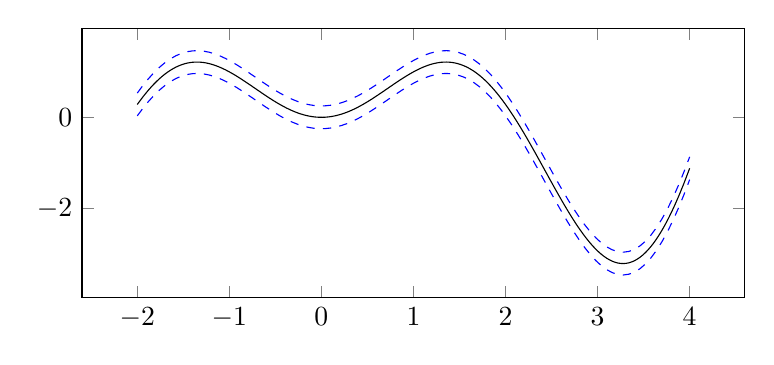
\begin{tikzpicture}
									\begin{axis}[domain=-2:4, samples=101, height=5cm, width=10cm]
		  								\addplot[thin, smooth] 		 { 			 ( x*sin( 1/2 * ( deg(3*x) ) ) ) };			
		  								\addplot[color=blue, dashed] { (  0.25 + ( x*sin( 1/2 * ( deg(3*x) ) ) ) ) };
		  								\addplot[color=blue, dashed] { ( -0.25 + ( x*sin( 1/2 * ( deg(3*x) ) ) ) ) };	
									\end{axis}
								\end{tikzpicture}
								\caption{$\epsilon$-Kugel um $f$ bzgl. $\| \cdot \|_{\infty}$}
							\end{center}
						\end{figure}
															
						Für $\epsilon \in (0, \min\{c_1 - a, b - c_2\})$ gilt dann $K(f, \epsilon) \subseteq A$, d.h. $A$ ist offen.
					\item Da punktweise Konvergenz durch Konvergenz bezüglich $\| \cdot \|_{\infty}$ impliziert wird, folgt direkt
						\[ \overline{A} \subseteq \{ f\in X \colon f(t) \in [a, b] \quad \forall t \in [a,b] \}. \]
						Ist umgekehrt $f \in X$ mit $f(t) \in [a, b]$ für alle $t \in [0,1]$, so definieren wir
						\[ f_{n}(t) = \begin{cases} a + \frac{1}{n} &, f(t) \leq a + \frac{1}{n} \\ b - \frac{1}{n} &, f(t) \geq b - \frac{1}{n} \\ f(t) &, \text{ sonst.}  \end{cases}   \]
						
						\begin{center}
						  \begin{figure}[H]
						  	\pgfmathdeclarefunction{p}{1}{\pgfmathparse{(x*sin(1/2*(deg(3*x))))}}
						  	\pgfmathdeclarefunction{f}{1}{\pgfmathparse{((and(p(#1)<=0.75, p(#1)>=-2.75)*p(#1)) + (and(p(#1)>0.75, p(#1)<=5.75)*0.75) + (and(p(#1)<-2.75, p(#1)>=-5.75)*-2.75))}}
							\begin{center}		
							  \begin{tikzpicture}
								\begin{axis}[domain=0:4,	 samples=101, height=5cm, width=10cm]
	    							\addplot [thin, dashed, smooth] {1.25} node [pos=1.25,pin={1:$b$},inner sep=0pt] {};
									\addplot [color=blue, thin, smooth] { ( x*sin(1/2*(deg(3*x))) ) };
									\addplot [thin, dashed, smooth] {-3.25} node [pos=-3.25,pin={1:$a$},inner sep=0pt] {};	
         							\addplot[color=red, thin, smooth]{f(x)};
								\end{axis}
							  \end{tikzpicture}
							\end{center}
							\caption{\textcolor{blue}{$f$} bzw. \textcolor{red}{$f_{n}$} für konkretes $n \in \MdN$}
						  \end{figure}
						\end{center}
						\[ \Rightarrow f_{n} \in A \text{ mit } \| f_{n} - f \|_{\infty} \rightarrow 0 \text{ } (n \rightarrow \infty) \text{, d.h. } f \in \bar A \]
					\item Aussage über $\partial A$ folgt aus \hyperref[bsp:4.11.b]{i)} und \hyperref[bsp:4.11.b]{ii)}
				\end{enumerate}
			\end{beweis}
		\item Sei $X$ ein normierter Vektorraum und $Y \subseteq X$ abzählbar mit $\overline{lin Y} = X$. Dann ist $X$ separabel.
			\begin{beweis}
				Wir definieren
				\[ lin_{\MdQ} Y \coloneqq \{ y = \sum_{i = 1}^{n} q_{j} y_{j} : q_{j} \in \MdQ \quad (q_{j} \in \MdQ + i \MdQ ), y_{j} \in Y, n \in \MdN \} \]
				Dann ist $lin Y$ abzählbar, da $Y$ abzählbar ist. Sei nun $\epsilon > 0$ beliebig, $x \in X$. \\
				Nach Voraussetzung existiert dann ein $y \in lin Y$ mit $\| x - y \| < \epsilon$ \\
				Zu diesem $y$ finden wir ein $z \in lin_{\MdQ} Y$ mit $\| y - z \| < \epsilon$
				\[ \Rightarrow \| x - z \| < 2 \epsilon, \quad \text{d.h. } \overline{lin_{\MdQ} Y} = X \]
			\end{beweis}
		\item $C[0, 1]$ ist separabel, da $ lin \{ t^{n}, n \in \MdN \} $ dicht in $C[0, 1]$ liegt nach dem Approximationssatz von Weierstrass.
		\item Die Räume $\ell^{p}, p \in [1, \infty)$ und $c_{0}$ sind separabel, da
			\[ D = lin \{ e_{k}, k \in \MdK \} \text{ dicht in allen Räumen liegt.} \]
		\item Der Raum $\ell^{\infty}$ ist nicht separabel: \\
			Die Menge $\Omega$ der $\{0, 1\}$-wertigen Folgen ist überabzählbar. Für $x, y \in \Omega$ mit $x \neq y$ gilt $\| x - y \|_{\infty} = 1$ \\
			Angenommen: $\overline{ \{v_{k}, k \in \MdN \} } = \ell^{\infty}$. Dann
			\[ \Omega \subseteq \bigcup_{k \in \MdN} K \left( v_{k}, \frac{1}{4} \right) \]
			Wegen $\| x - y\|_{\ell^{\infty}} = 1$ $\forall x, y \in \Omega$ kann aber in jeder Kugel $K(v_{k}, \frac{1}{4})$ nur ein Element auf $\Omega$ liegen. 
			(d.h. zu $x \in \Omega$ existiert ein $k(x) \in \MdK$ mit $x \in K(v_{k(x)}, \frac{1}{4})$) \\
			$\Rightarrow$ die Abbildung $ J \colon \Omega \rightarrow \MdN, x \rightarrow k(x)$ ist injektiv \\
			$\Rightarrow \Omega$ ist abzählbar, Widerspruch.
	\end{enumerate}
\end{beispiel}


Schlie{\ss}lich betrachten wir noch die Stetigkeit:


\begin{definition}
	Seien $(M, d_{M}), (N, d_{N})$ metrische Räume. \\
	Eine Abbildung $f \colon M \rightarrow N$ hei{\ss}t \textbf{stetig in $x_{0} \in M$}, falls für alle $(x_{n}) \subset M$ gilt
	\[ x_{n} \rightarrow x_{0} \text{ in } M \Rightarrow f(x_{n}) \rightarrow f(x_{0}) \text{ in } N \]
	\[ (d_{M}(x_{n}, x_{0}) \rightarrow 0 \hspace{0.25cm} (n \rightarrow \infty) \hspace{0.5cm} \Rightarrow \hspace{0.5cm} d_{N}(f(x_{n}), f(x_{0})) \rightarrow \hspace{0.25cm} (n \rightarrow \infty)) \]
	Die Abbildung $f$ hei{\ss}t \begriff{stetig} \textbf{auf $M$}, falls $f$ in jedem Punkt von $M$ stetig ist.
\end{definition}


Hierfür gelten folgende Eigenschaften:


\begin{prop} \label{prop:4.13}
	Sei $(K,d_{K}), (M, d_{M})$ und $(N, d_{N})$ metrische Räume und $f \colon M \rightarrow N, g \colon K \rightarrow M$. Dann gilt:
	\begin{enumerate}[label=\alph*\upshape)]
		\item Ist $g$ stetig in $x_{0}$, $f$ stetig in $g(x_{0})$, dann ist auch 
			\[ f \circ g \colon K \rightarrow N \text{ stetig in } x_{0} \]
		\item \label{prop:4.13.b} $f$ ist stetig in $x_{0} \in M$ genau dann, wenn 
			\[ \forall \epsilon > 0 \hspace{0.15cm} \exists \delta > 0 \hspace{0.15cm} \forall x \in M \text{ mit } d_{M}(x, x_{0}) < \delta \text{ gilt } d_{N}(f(x), f(x_{0})) < \epsilon \]
		\item Die folgenden Aussagen sind äquivalent:
			\begin{enumerate}
				\item $f$ ist stetig auf $M$
				\item Ist $U \subset N$ offen, so ist auch $f^{-1}(U)$ offen in $M$
				\item Ist $A \subset N$ abgeschlossen, so ist auch $f^{-1}(A)$ abgeschlossen in $M$.
			\end{enumerate}
	\end{enumerate}	
	\begin{beweis}		
		\begin{enumerate}[label=\alph*\upshape)]	
			\item Folgt direkt aus der Definition
			\item $" \Rightarrow "$: Annahme, das $\epsilon$-$\delta$-Kriterium gilt nicht. Dann existiert ein $\epsilon > 0$ und für jedes $n \in \MdN$ ein $x_{n} \in K(x_{0}, \frac{1}{n})$ mit $d_{M}(f(x_{n}), f(x_{0})) \geq \epsilon$. \\
				Dann gilt aber $d_{M}(x_{n}, x_{0}) < \frac{1}{n} \rightarrow 0$ für $n \rightarrow \infty$ und $d_{N}(f(x_{n}, f(x_{0})) \geq \epsilon \not\rightarrow 0$ für $n \rightarrow \infty$, d.h. $f$ ist nicht stetig in $x_{0}$. \\ \\
				$" \Leftarrow "$: Es gelte das $\epsilon$-$\delta$-Kriterium. Sei $(x_{n}) \subseteq M$ mit $x_{n} \rightarrow x_{0}, \epsilon > 0$. \\
				Dann gilt $d_{N}(f(x_{n}), f(x_{0})) < \epsilon$ für $n$ gro{\ss} genug. Da $\epsilon > 0$ beliebig, folgt $d_{N}(f(x_{n}), f(f_{0})) \rightarrow 0$ für $n \rightarrow \infty$.
			\item $(i) \Rightarrow (iii)$: Sei $A \subseteq N$ abgeschlossen und $(x_{n}) \subseteq f^{-1}(A)$ mit $x_{n} \rightarrow x$ in $M$ für $n \rightarrow \infty$. Dann gilt nach $(i)$ $f(x_{n}) \rightarrow f(x)$ in $N$ für $n \rightarrow \infty$. \\
				Da $(f(x_{n}))_{n \geq 1} \subseteq A$ und $A$ abgeschlossen ist, folgt $f(x) \in A$, d.h. $x \in f^{-1}(A)$. \\
				Also ist $f^{-1}(A)$ abgeschlossen. \\ \\
				$(iii) \Rightarrow (ii)$: Sei $U \subset N$ offen $\Rightarrow$ $U^{c}$ abgeschlossen $\Rightarrow$ $f^{-1}(U^{c}) = f^{-1}(U)^{c}$ ist abgeschlossen $\Rightarrow$ $f^{-1}(U)$ offen. \\ \\
				$(ii) \Rightarrow (i)$: 	Sei $x_{0} \in M$ beliebig. Für $\epsilon > 0$ ist nach $(ii)$ dann auch $f^{-1}(K(f(x_{0}), \epsilon))$ offen in M. \\
				Da $x_{0} \in f^{-1}(K(f(x_{0}), \epsilon))$, existiert ein $\delta > 0$ mit $K(x_{0}, \delta) \subseteq f^{-1}(K(f(x_{0}),\epsilon))$\\
				Das bedeutet gerade
				\[ \forall \epsilon > 0 \text{ } \exists \delta > 0: \forall x \in M \text{ mit } d_{M}(x_{0}, x) < \delta \text{ gilt auch} \]
				\[ d_{N}(f(x_{0}), f(x)) < \epsilon \]
				Nach \hyperref[prop:4.13.b]{b)} bedeutet dies gerade, dass $f$ stetig in $x_{0}$ ist.
		\end{enumerate}
	\end{beweis}
\end{prop}


\begin{beispiel}
	\begin{enumerate}[label=\alph*\upshape)]
		\item Sind $(M_{1}, d_{1})$ und $(M_{2}, d_{2})$ metrische Räume, so definiert
				\[ d(x, y) \coloneqq d_{1}(x_{1}, y_{1}) + d_{2}(x_{2}, y_{2}) \]
			für $x = (x_{1}, x_{2}), y = (y_{1}, y_{2}) \in M_{1} \times M_{2}$ eine Metrik mit
			\[ d(x_{n}, x) \rightarrow 0 \gdw d_{1}(x_{n,1}, x_{1}) \rightarrow 0, d_{2}(x_{n,2}, x_{2}) \rightarrow 0 \]
			In diesem Sinne ist jede Metrik $d: M \times M \rightarrow \MdR$ stetig. Denn: \\
			Sei $(x_{n}, y_{n}) \rightarrow (x, y)$ in $M \times M$, d.h.
			\[ d(x_{n}, x) \rightarrow 0 \text{ und } d(y_{n}, y) \rightarrow 0 \hspace{0.5cm} (n \rightarrow \infty) \]
			\begin{align*}
				 d(x_{n}, y_{n}) - d(x, y) & \leq d(x_{n}, x) + d(x, y_{n}) - d(x, y) \\
										  & \leq d(x_{n}, x) + d(x, y) + d(y, y_{n}) - d(x, y) 		
			\end{align*}
			\[ d(x, y)- d(x_{n}, y_{n}) \leq \dotsc \leq d(x, x_{n}) + d(y_{n}, y) \]
			\[ \Rightarrow | d(x, y) - d(x_{n}, y_{n}) | \leq d(x, x_{n}) + d(y_{n}, y) \rightarrow 0 \hspace{0.5cm} (n \rightarrow \infty) \]
		\item Sei $X$ ein normierter Vektorraum und
			\begin{align*}
				A \colon \MdK \times X \rightarrow X, & \hspace{0.5cm} A( \alpha, x) = \alpha x \\
				S \colon X \times X \rightarrow X, & \hspace{0.5cm} S(x, y) = x + y
			\end{align*}
			Dann sind $A$ und $S$ stetig.
		\item Sei $X = C[0, 1], t_{0} \in [0, 1], \psi \colon X \rightarrow \MdK, \psi(f) = f(t_{0})$ \\
		Nach \hyperref[bsp:1-3.15]{Beispiel 3.15} ist $\psi$ stetig. D.h. ist $A \subset \MdK$ offen (abgeschlossen), so ist $\psi^{-1}(A)$ offen (abgeschlossen) nach \hyperref[prop:4.13]{Proposition 4.13}.
	\end{enumerate}	
\end{beispiel}



\newpage
%!TEX root = Funktionalanalysis - Vorlesung.tex

\chapter{Vollst{\"a}ndigkeit}

\begin{definition}
	Sei $(M, d)$ ein metrischer Raum.
	\begin{enumerate}[label=\alph*\upshape)] \index{Cauchy-Folge} \index{vollständig} \index{Banachraum}
		\item $x_{n} \in M$ hei{\ss}t \textbf{Cauchy-Folge}, falls es zu jedem $\epsilon > 0$ ein $n_{0} \in \MdN$ gibt, sodass $\forall m, n \geq n_{0}$ gilt:
			\[ d(x_{n}, x_{m}) \leq \epsilon \]
		\item $(M, d)$ hei{\ss}t \textbf{vollständig}, falls jede Cauchyfolge $(x_{n}) \subset M$ einen Grenzwert \uline{in M} hat:
			\[ \lim_{n \rightarrow \infty} x_{n} = x \quad x \in M \]
		\item Ein normierter Raum $(X, \| \cdot \|)$, der vollständig ist bezüglich $d(x, y) = \| x - y \|$ heißt \textbf{Banachraum}.
	\end{enumerate}
\end{definition}

\begin{bemerkung}
	\begin{enumerate}[label=\alph*\upshape)]
		\item Jede konvergenzte Folge in $(M, d)$ ist eine Cauchy-Folge:
			\[ \text{Sei } \lim_{n \rightarrow \infty} x_{n} = x: \quad d(x_{n}, x_{m}) \leq d(x_{n}, x) + d(x, x_{m}) \xrightarrow[n, m \rightarrow \infty]{} 0 \]
		\item \uline{Aber:} nicht jede Cauchy-Folge eines normierten Raums $X$ konvergiert in $X$
			\begin{beispiel*}
				$X = C[0, 2], \quad \| f \|_{1} = \int_{0}^{2} | f(t) | dt, \quad
				f_{n}(x) = \begin{cases}x^{n} & \text{ für } x \in [0, 1] \\ 1 & \text{ für } x \in [1, 2]\end{cases}$	
				\[ f_{n}(x) \rightarrow f(x) = \begin{cases} 0 & \text{ für } x \in [0, 1) \\ 1 & \text{ für } x \in [1, 2] \end{cases} \quad \text{ für feste } x \in [0, 2] \]
				Nach dem Satz von Lebesgue folgt $\| f - f_{n} \|_{1} \rightarrow 0$ für $n \rightarrow \infty$, aber $f \notin C[0, 2]$ \\
				Demnach ist $f_{n}$ zwar eine Cauchy-Folge, aber $f_{n}$ konvergiert nicht gegen $f$ in $X$ bezüglich der $\| \cdot \|_{1}$-Norm.
			\end{beispiel*}
	\end{enumerate}	
\end{bemerkung}

\begin{prop}
	Sei $X$ ein metrischer Raum, $Y$ ei Banachraum.
	\[ C(x, Y) = \{ f : X \rightarrow Y: f \text{ stetig} \}, \quad \| f \|_{\infty} = \sup_{x \in X} \| f(x) \|_{Y} \]
	Dann ist $C(X, Y)$ ein (linearer) Banachraum.
\end{prop}

\begin{beispiel*}
	$\Omega \subseteq \MdR^{n}, \quad C(\Omega, \MdR)$
	\begin{beweis}
		Sei $(f_{n})$ eine Cauchy-Folge in $C(X, Y)$. \\
		Für alle $x \in X$:
		\[ \| f_{n}(x) - f_{m}(x) \|_{Y} \leq \| f_{n} - f_{m} \|_{\infty} \xrightarrow[n, m \rightarrow \infty]{} 0 \]
		Für alle $x \in X$: $(f(x))_{n \in \MdN}$ ist eine Cauchy-Folge in $Y$.
		da $Y$ vollständig ist, existiert $f(x) := \lim_{n \rightarrow \infty} f_{n}(x)$ in Y. \\ \\
		z.z. $f \in C(X, Y), \quad \| f - f_{n} \|_{\infty} \rightarrow 0$. \\
		Zu $\epsilon > 0$ gibt es ein $n_{0}$, sodass für alle $x \in X$:
		\[ \| f_{n}(x) - f_{m}(x) \|_{Y} \leq \| f_{n} - f_{m} \|_{\infty} \leq \epsilon \]
		Für jedes $x \in X$ fest folgt für $m \rightarrow \infty$:
		 \[ \| f_{n}(x) - f(x) \| \leq \epsilon \quad \text{ für } n \geq n_{0} \]
		 \[ \Rightarrow \| f_{n} - f \|_{\infty} \leq \epsilon \text{ für } n \geq n_{0} \quad  \text{ nehme das Supremum über } x \in X \]
		 $f \in C(X, Y)$, da der gleichmä{\ss}ige Limes stetiger Funktionen stetig ist.
	\end{beweis}
\end{beispiel*}

\begin{beispiel}
	Sei $\Omega \subseteq \MdR^{n}$ offen und beschränkt. $C^{m}(\bar \Omega)$ ist vollständig bezüglich der Supremums-Norm.	
	\begin{beweis}
		Für $C^{1}(\bar \Omega)$ gilt $\| f \|_{C^{1}} = \| f \|_{\infty} + \sum_{i = 1}^{n}  \| \frac{\partial}{\partial x_{i}} f \|_{\infty}$. \\
		 Sei $(f_{j}) \subset F$ in $C^{1}(\bar \Omega)$.
		 \[ \Rightarrow (f_{j})_{j \in \MdN}, \quad (\frac{\partial}{\partial x_{j}} f_{j})_{j \in \MdN}, \quad i = 1, \dotsc, n \text{ Cauchy-Folgen in } C(\bar \Omega) \]
		 Da $C(\bar \Omega)$ vollständig ist, existieren für $i \in \{ 1, \dotsc, n \} $
		 	\begin{align*}
		 		f & = \lim_{j \rightarrow \infty} f_{j} \\
		 		g_{i} & = \lim_{j \rightarrow \infty} \frac{\partial}{\partial x_{i}} f_{j}
		 	\end{align*}
		 in $C(\bar \Omega)$. Setze $g = (g_{1}, \dotsc, g_{n})$ \\ \\
		 z. z. $f \in C^{1}(\bar \Omega)$ und $g = \nabla f$ \\
		 Beweis: zu $u \in \Omega$ und $v$ nahe bei $u$ wähle
		 \[ u_{t} = (1 - t) u + t v \]
		 \begin{align*}
		 	| f_{k}(v) - f_{k} (u) - \nabla f_{k}(u) (v - u) | & = | \int_{0}^{1} [ \nabla f_{k} (u_{t}) - \nabla f_{k} (u) ] (v - u) dt \\
		 		& \leq  \int_{0}^{1} | \nabla f_{k} (u_{t}) - \nabla f_{k} (u) | dt (v - u) \\
		 		& \leq \left[ \int_{0}^{1} | \nabla f_{k}(u_{t}) - g(u_{t}) | dt + \int_{0}^{1} | g(u_{t}) - g(u) | dt + \int_{0}^{1} | g(u) - \nabla f_{k}(u) | dt \right] |v - u| \\
		 		& \leq \left[ z \| \nabla f_{k} - g \|_{\infty} + \sup_{0 \leq t \leq 1} | g(u_{t}) - g(u) | \right] |v - u|
 		 \end{align*}
 		 \begin{align*}
 		 	\text{für } k \rightarrow \infty: | f(v) - f(u) - g(u)(v - u) | & \leq \sup_{t \in [0, 1]} | g(u_{t}) - g(u) | |v - u| \\
 		 		& \rightarrow 0 \text{ für } v \rightarrow u \text{ (da g gleichmä{\ss}ig stetig)}
 		 \end{align*} 
	\end{beweis}
\end{beispiel}

\begin{bemerkung}
	\begin{enumerate}[label=\alph*\upshape)]
		\item $\| \cdot \|_{1}, \| \cdot \|_{2}$ seien äquivalente Normen auf $X$. Ist $X$ bezüglich $\| \cdot \|_{1}$, so auch bezüglich $\| \cdot \|_{2}$.
			\begin{beweis}
				Äquivalente Normen haben gleiche Cauchy-Folgen.
			\end{beweis}
			Bsp.: $C^{1}[0, 1]$, $\vertiii{f} = |f(0)| + \sup_{t \in [0, 1]} | f'(t) |$. Früher: $\vertiii{\cdot} \tilde \| \cdot \|_{\infty} \Rightarrow \left( C[0, 1], \vertiii{\cdot} \right)$ ist vollständig.
		\item Abgeschlossene Teilmengen von 	Banachräumen sind vollständige metrische Räume bezüglich $d(x, y) = \| x - y\|$
			\begin{beweis}
				$(x_{n}) \subset M$, Cauchy-Folge in $X \Rightarrow \lim_{n \rightarrow \infty} x_{n} = x \in X \xRightarrow[M abg.]{} x \in M$ existiert.	
			\end{beweis}
			Bsp.: $X = C([0, 1], \MdC), M = \{ f \in X: |f ( t )| = 1 \}$ ist ein vollständiger metrischer Raum.
	\end{enumerate}
\end{bemerkung}



\begin{satz}
	Sei $X$ ein normiert Raum, $Y$ ein Banachraum.
	Dann ist $B(X, Y)$ mit der Operatornorm vollständig. \\
	Insbesondere: $X' = B(X, \MdK)$ ist immer  vollständig.
\end{satz}
\begin{beweis}
	Sei $(T_{n}) \subset B(X, Y)$ eine Cauchy-Folge bezüglich der Operatornorm. Sei $x \in X$
	\[ \| T_{n} x - T_{m} \|_{Y} \leq \| T_{n} - T_{m} \| \|x\|_{X} \]
	Also $(T_{n}x)_{n \in \MdN}$ eine Cauchy-Folge in $Y$ für alle $x \in X$. Definiere $T x : = \lim_{n \rightarrow \infty} T_{n} x$ \\
	z.z. $T \in B(X, Y),$ $s\| T_{n} - T \| \rightarrow 0$ \\
	\[ T_{n} (x + y)  = T_{n} x + T_{n} y \xrightarrow[n \rightarrow \infty]{} T(x + y) = Tx + Ty \]
	\begin{align*}
		\| Tx - T_{n}x \| & \overset{Norm \text{ } stetig}{=} \lim_{m \rightarrow \infty} \| T_{m} x - T_{n} x \| \\
		 & \leq \lim_{m \rightarrow \infty} \| T_{n} - T_{m} \| \| x \| \\
		 & \leq \epsilon \| x \| \text{ für n gro{\ss} genug.}
	\end{align*}
	Wobei $\| T - T_{n} \| \leq \epsilon$ für $n$ gro{\ss} genug.
	Also für $\| x \| \leq 1$:
	\[ \| T x \| \leq \| T_{n} x \| + \epsilon \leq \| T_{n} \| + \epsilon  \]
	\[ \Rightarrow \| T \| \leq \| T_{n} \| + \epsilon, \quad \text{ also } T \in B(X, Y) \]
\end{beweis}

\begin{bemerkung}[Exponentialfunktion]
	$A \in B(X)$, $X$ Banachraum
	\begin{itemize}
		\item Frage: $e^{tA}$
		\item Idee: $e^{tA} = \sum_{n = 0}^{\infty} \frac{1}{n!} t^{n} A^{n}$
		\item Setze $S_{m} = \sum_{n = 0}^{m}	 \frac{1}{n!} t^{n} A^{n}$
	\end{itemize}
	z. z. $S_{m}$ ist eine Cauchy-Folge in $B(X)$ \\
	Seien $k, m \in \MdN, k > 0$
	\begin{align*}
		\| S_{k} - S_{m} \| & \leq \sum_{n = m +1}^{k} \| \frac{1}{n!} t^{n} A^{n} \| \\
			& \leq \sum_{n = m +1}^{k}  \frac{1}{n!} | t^{n} | \| A^{n} \| \xrightarrow[k, m \rightarrow \infty]{} 0
	\end{align*}
	Da $B(X)$ vollständig ist, ist $e^{tA} = \lim_{m \rightarrow \infty} S_{m}$ in $B(X)$.
\end{bemerkung}

\begin{prop}[Neumann'sche Reihe] \label{prop:1-5.8-NMR}
	Sei $A \in B(X)$, $X$ ein Banachraum mit $\| A \| < 1$. \\
	Dann ist $Id - A$ invertierbar und 
	\[ \left( Id - A \right)^{-1} = \sum_{n = 0}^{\infty} A^{n} \]
	\begin{beweis}
		$S_{m} = \sum_{n = 0}^{m} A^{n}$ ist eine Cauchy-Folge in $B(X)$, denn für
		\begin{align*}
		k > m: \quad \| S_{k} - S_{m} \| & \leq \sum_{n = m + 1}^{k} \| A^{n} \| \\
			& \leq \sum_{n = m + 1}^{k} \| A \|^{n} \rightarrow 0 \text{ für } m, n \rightarrow \infty \text{, da} \| A \| < 1
		\end{align*}
		$R := \lim_{m \rightarrow \infty} S_{m}$ existiert in $B(X)$, da $B(X)$ vollständig.
		\[ S_{m} (Id - A) = (Id - A) S_{m} = Id - A^{m} \]
		mit $\| A^{m} \| \leq \| A \|^{m} \rightarrow 0 \text{ für } m \rightarrow \infty$
		\[ \Rightarrow R (Id - A) = (Id - A) R = Id, \quad R = (Id - A)^{-1} \]
	\end{beweis}
\end{prop}

\begin{kor}
	$X$ sei ein Banachraum und $J: X \rightarrow X$ ein (surjektiver) Isomorphismus. \\
	Für $A \in B(X)$ und $\| A \| < \| J^{-1} \|^{-1}$ ist auch $J - A$ ein Isomorphismus \\ \\
	Insbesondere: $G = \{ T \in B(X): T \text{ stetig und invertierbar} \}$ ist eine offene Menge in $B(X)$.
	\begin{beweis}
		Da $J - A = J (Id - J^{-}A) $ folgt:
		\[ \| J^{-1} A \| \leq \| J^{-1} \| \underbrace{\| A \|}_{< \| J^{-1} \|^{-1}} < 1 \]
		Nach \hyperref[prop:1-5.8-NMR]{5.8} ist $(Id - J^{-1} A)$ invertierbar mit
			\begin{align*}
				(J - A)^{-1} & = (Id - J^{-1} A)^{-1} J^{-1} \\
					& = \sum_{n = 0}^{\infty} (J^{-1} A)^{n} J^{-1}
			\end{align*}
	\end{beweis}
\end{kor}

\begin{prop} \label{prop:1-5.10}
	Sei $X$ ein normierter Raum, $Y$ ein Banachraum und $D \subset X$ ein dichter Teilraum. \\
	Jeder linearere Operator $T: X \rightarrow Y$ mit
		\[ \| T x \|_{Y} \leq M \| x \|_{X}, \quad \text{ für alle } x \in D \]
	lässt sich zu einem eindeutig bestimmten Operator $ \tilde T \in B(X, Y)$ mit $\| \tilde T \| \leq c$ fortsetzen.	
\end{prop}

\begin{kor} \label{kor:1-5.11}
	Sei $X$ ein normierter Banachraum, $D \subset X$ dicht in $X$ und sei eine Folge $T_{n} \in B(X, Y)$, wobei $(T_{n} x)$ eine Cauchy-Folge für jedes $x \in D$ sei. \\
		Dann gibt es genau einen Operator $T \in B(X, Y)$ mit
		\[ \lim_{n \rightarrow \infty} T_{n} x = T x \]
	\begin{beweis}
		Setze für $x \in D$: $Tx = \lim_{n \rightarrow \infty} T_{n}(x)$, da $Y$ vollständig. \\
		Dieses $T: X \rightarrow Y$ ist linear. \\
		Nach \hyperref[prop:1-5.10]{5.10} gibt es genau ein $\tilde T \in B(X, Y)$ mit $\tilde T x = T x$ für $x \in D$, $\| \tilde T \| \leq M$, denn für $x \in D$:
		\[ \| T x \| \leq \limsup \| T_{n} x \| \leq M \| x \| \]
		z. z. $\tilde T x = \lim_{n \rightarrow \infty} T_{n} x$ für alle $x \in X$. \\
		Zu $\epsilon > 0$ wähle $y \in D$ mit $\| x - y \| \leq \frac{\epsilon}{2 M}$. Dann:
		\begin{align*}
			\| \tilde T x - T_{n} x \| & \leq \| \tilde T x - T y \| + \| T y - T_{n} y \| +  \| T_{n} y - T_{n} x \| \\
				& \leq \| \tilde T \| \| x - y \| + \| T y - T_{n} y \| + \| T_{n} \| \| x - y\| 
		\end{align*}
		\[ \limsup_{n \rightarrow \infty}  \| \tilde T x - T_{n} x \| \leq M \frac{\epsilon}{2 M} + \limsup_{n \rightarrow \infty} \| T y - T_{n} y \| + M \frac{\epsilon}{2 M} \leq \epsilon + 0 \]
	\end{beweis}
\end{kor}

\begin{beispiel}
	$e_{n} (t) = e^{2 \pi n i t} = \cos(2 \pi n t) + i \sin(2 \pi n t), \quad D = \{ (\alpha_{n}) \in L^{2}(\MdZ):$ Nur endlich viele $\alpha_{n} \neq 0 \}$
	\[ T : \begin{cases} D \rightarrow L^{2}[0, 1] \\ (\alpha_{n}) \rightarrow \sum_{n \in \MdZ} \alpha_{n} e_{n} \end{cases} \]
	Wie kann man man unendlich Reihen $\sum_{n \in \MdZ} \alpha_{n} e_{n}$ definieren? \\
	Ohne Beweis aus der Fourieranalysis:
	\begin{itemize}
		\item Es gibt $(\alpha_{n}) \in \MdC^{2}$, so dass $\sum_{n \in \MdZ} \alpha_{n} e_{n}(t)$ nicht für alle $t \in [0, 1]$ konvergent.
		\item Für alle $(\alpha_{n}) \in \MdC^{2}$ konvergiert $\sum_{n \in \MdZ} \alpha_{n} e_{n}(t)$ punktweise für fast alle t $t \in [0, 1]$
		\item $\int_{0}^{1} e_{n} \overline e_{m} dt = \delta_{n, m}$
	\end{itemize}
	Für $(\alpha_{n}) \in D$ wie in der Linearen Algebra folgt:
	\begin{align*}
		\| \sum_{n} \alpha_{n} e_{n}(t) \|_{L^{2}[0, 1]}^{2} & = \int (\sum_{n} \alpha_{n} e_{n}(t)) \overline{(\sum_{m} \alpha_{m} e_{m}(t))} dt \\
		& = \sum_{n, m} \alpha_{n} \alpha_{m} \int e_{n}(t) \overline{e_{m}(t)} dt \\
		& = \sum_{n} |\alpha_{n}|^2
	\end{align*}
	D.h. $\| T (\alpha_{n}) \| \leq 1 \left( \sum_{n} |\alpha_{n}|^2 \right)^{\frac{1}{2}} = \| \alpha_{n} \|_{L^{2}}$, $(M = 1)$. Nach \hyperref[prop:1-5.10]{5.10} gibt es dann ein $\tilde T: \ell^{2}[0, 1] \rightarrow L^{2}(0, 1)$ mit $\| \tilde T \| \leq 1$ \\ \\
	\uline{Zusatz:} $T_{m}((\alpha_{n})) = \sum_{n = m}^{\infty} \alpha_{n} e_{n}$. $T_{m}: \ell^{2} \rightarrow L^{2}[0, 1],$ $\| Tm \| \leq 1$ \\
	Für $(\alpha_{n}) \in \ell^{2}$ gilt: $T (\alpha_{n}) = \lim_{m \rightarrow \infty} T_{m}(\alpha_{n})$. \\
	Nach \hyperref[kor:1-5.11]{Kor. 11}: $T_{m}(\alpha_{n}) \rightarrow T (\alpha_{n})$ in $L^{2}[0, 1]$ für alle $(\alpha_{n}) \in \ell^{2}$. Damit konvergiert die Partialsumme der Fourierreihen in $L^{2}[0, 1]$.
\end{beispiel}

\begin{prop}
	\begin{enumerate}[label=\alph*\upshape)]
		\item upcoming
	\end{enumerate}	
\end{prop}


\newpage































%!TEX root = Funktionalanalysis - Vorlesung.tex



\section{Kompakte Mengen}



\begin{definition} \index{kompakt} \index{relativ kompakt}
	Sei $(M, d)$ ein metrischer Raum. Eine Menge $K \subseteq M$ hei{\ss}t (folgen-)\begriff{kompakt}, falls es in jeder Folge $(x_{n}) \subset M$ eine Teilfolge $(x_{n_{k}})$ und ein $x \in K$ gibt, so dass 
		\[ \lim_{k \rightarrow \infty} x_{n_{k}} = x \]
		$K \subseteq M$ hei{\ss}t \begriff{relativ kompakt}, falls $\overline{K}$ in $M$ kompakt ist.
\end{definition}


\begin{satz} \label{satz-6.2}
	Sei $X$ ein normierter Vektorraum. Dann ist
	\[ \overline{U_{x}} = \{ x \in X: \| x \| \leq 1 \} \]
	genau dann kompakt, wenn $dim X < \infty$.
\end{satz}
 
\begin{beweis}
	$"\Rightarrow"$ $X \cong \MdK^{d}$, $d = \dim X$, $U_X$ ist abgeschlossen, beschränkt $\xRightarrow[Borell]{Heine-} U_{X}$ ist kompakt. \\ \\
	$"\Leftarrow"$ Sei $\dim X = \infty$. Wähle $x_1 \in X$ mig $\| x_1 \| = 1$. \\
	Nach \eqref{lemma:6.3-Riesz} mit $ Y = \overline{span}\{ x_{1} \}$ finde zu $\delta = \frac{1}{2}$ ein $x_{2} \in X, \| x_{2} \| = 1$ und $\| x_{2} - x_{1} \| \geq \frac{1}{2}$ \\
	Wieder nach \eqref{lemma:6.3-Riesz} mit $ Y = \overline{span}\{ x_{1}, x_{2} \}$ finde zu $\delta = \frac{1}{2}$ ein $x_{3} \in X, \| x_{3} \| = 1$ und $\| x_{3} - x_{j} \| \geq \frac{1}{2}$ für $j = 1, 2$ \\
	Induktiv erhält man eine Folge $x_{i} \in X$ mit $\| x_{i} \| = 1$ und $\| x_{i} - x_{j} \| \geq \frac{1}{2}$ für $j = 1, \dotsc, i - 1$.
	Dieses Folge $(x_{i})_{i \geq 1}$ hat keine Teilfolge, die eine Cauchy-Folge ist und demnach ist $U_{X}$ nicht relativ kompakt in $X$. 
\end{beweis}


\begin{lemma}[Riesz] \label{lemma:6.3-Riesz} \index{Riesz}
	Sei $Y$ ein abgeschlossener Teilraum von $X$ und $X \neq Y$. Zu $\delta \in (0, 1)$ existiert ein $x_{\delta} \in X \setminus Y$, sodass
	\[ \| x \| = 1, \quad \| x_{\delta} - y\| \geq 1 - \delta \quad \text{ für alle } y \in Y \]
\end{lemma}

\begin{beweis}
	Sei $x \in X \setminus Y$ und $d \coloneqq \inf \{ \| x - y \|: y \in Y \} > 0$, da $Y$ ein abgeschlossener Teilraum ist. \\
	Da $ d < \frac{d}{1 - \delta}$ gibt es ein $y_{\delta} \in Y$ mit $\| x - y_{\delta} \| < \frac{d}{1 -  \delta}$. \\ 
	Setze $x_{\delta} = \frac{x - y_{\delta}}{\| x - y_{\delta} \|}$, damit gilt $\| x_{\delta} \| = 1$ und weiter 
	\begin{align*}
		\| x_{\delta} - y \| & = \| \frac{x}{\| x - y_{\delta} \|} - \frac{y_\delta}{\| x - y_{\delta} - y\|} \|	\\
			& = \frac{1}{\| x - y_{\delta} \|} \| x - \underbrace{y_{\delta} - \| x - y_{\delta} \| y}_{\leq y} \| \\
			& \geq \frac{d}{\| x - y_{\delta} \|} \\
			& \geq 1 - \delta
	\end{align*}
\end{beweis}


\begin{beispiel} \label{bsp:6.4}
	Sei $X = \ell^{p}$ für $1 \leq p < \infty$ gilt: \\
	$M \subset \ell^{p}$ ist kompakt genau dann, wenn
	\[ \sup \{ \sum_{ n = 1}^{\infty} |x_{n}|^{p} : x = (x_{m}) \in M \} \xrightarrow[k \rightarrow \infty]{} 0 \]	
	(Kompakte Mengen lassen sich gut durch endliche Mengen approximieren)
\end{beispiel}

\begin{beweis}
	siehe Übung.	
\end{beweis}


\begin{satz} \label{satz:6.5}
	Sei $(M, d)$ ein metrischer Raum . Für $k \subset M$ sind folgende Aussagen äquivalent:
	\begin{enumerate}[label=\alph*\upshape)]
		\label{satz:6.5a}
		\item $K$ ist (folgen-)kompakt 
		\label{satz:6.5b}
		\item $K$ ist vollständig und total beschränkt, d.h. für alle $\epsilon > 0$ gibt es endlich viele $x_{1}, \dotsc, x_{m} \in M$ so dass
			\[ K \subset \bigcup_{j = 1}^{m} K(x_{j}, \epsilon) \]
		\label{satz:6.5c}
		\item Jede Überdeckung von $K$ durch offene Mengen $U_{j}, j \in J$ mit $K \subset \bigcup_{j \in J} U_{j}$ besitzt eine endliche Teilüberdeckung, d.h. $j_{1}, \dotsc, j_{m}$ mit
			\[ K \subset \bigcup_{k = 1}^{m} U_{j_{k}} \]
	\end{enumerate}
\end{satz}

\begin{beweis}
	$a) \Rightarrow  b)$ (indirekt) \\
	Angenommen $b)$ ist falsch. Dann gibt es ein $\epsilon > 0$, so dass für alle $x_{1}, \dotsc, x_{n}, n \in \MdN$ gilt:
	\[ K \not\subset K(x_{1}, \epsilon) \cup \dotsc \cup K(x_{n}, \epsilon) \]
	Um einen Widerspruch zu erhalten konstruieren wir eine Folge ohne konvergente Teilfolge: \\
	Wähle $y_{1} \in K$ beliebig, dann gilt nach Voraussetzung $K \not\subset K(y_{1}, \epsilon)$.
	Wähle weiter $y_{2} \in K \setminus K(y_{1}, \epsilon)$ beliebig, dann gilt $K \not\subset K(y_{1}, \epsilon) \cup K(y_{2}, \epsilon)$. \\
	Induktiv erhält man eine Folge $y_{j} \in K$ mit $y_{j} \notin \{ K(y_{1}, \epsilon) \cup \dotsc \cup K(y_{j - 1}, \epsilon \}$. \\
	D.h. $\|y_{j} - y_{k} \| \geq \epsilon$ für $k = 1, \dotsc, j - 1$. D.h. $y_{j}$ hat keine konvergente Teilfolge, was ein Widerspruch zu $a)$ ist. \\ \\
	$b) \Rightarrow c)$ (indirekt) \\
	Sei $c)$ falsch, d.h. es gibt eine offene Überdeckung $K \subset \bigcup_{j \in J} U_{j}$ ohne endliche Teilüberdeckung.
	Zu $\epsilon_{1}$ gibt es nach $b)$ aber endlich viele $x_{1}^{1}, ..., x_{m}^{1} \in K$, so dass 
	\[ K \subset \bigcup_{j = 1}^{m} K(x_{j}^{1}, \epsilon_{1}) \]
	Setze der Kürze halber $y_{1} \coloneqq x_{j_{0}}^{1}$. Nun gibt es eine dieser Kugeln $K(y_{1}, \epsilon_{1})$, sodass $\underbrace{K \cap K(y_{1}, 1)}_{=: L_{1}}$ nicht durch endlich viele der $U_{j}$ überdeckt werden kann. \\
	Nach $B)$ gibt es aber auch zu $\epsilon_{2} = \frac{1}{2}$ endlich viele $x_{1}^{2}, \dotsc, x_{m'}^{2}$, sodass 
	\[ L_{1} \subset K(x_{1}^{2}, \epsilon_{2}) \cup \dotsc \cup K(x_{m'}^{2}, \epsilon_{2}). \] 
	Wieder muss es nach Voraussetzung eine dieser Kugeln $K(y_{2}, \epsilon_{2})$ geben, sodass $\underbrace{K \cap K(y_{1}, \epsilon_{1}) \cap K(y_{2}, \epsilon_{2})}_{=: L_{2}}$ sich nicht durch endlich viele der $U_{j}$ überdecken lässt. \\
	Induktiv finden wir zu $\epsilon_{l} = \frac{1}{2^{l - 1}}$ eine Folge $y_{l} \in K$, so dass
	\[ L_{l} \coloneqq K \cap K(y_{1}, \epsilon_{1}) \cap \dotsc \cap K(y_{l}, \epsilon_{l}) \]
	sich nicht durch endlich viele der $U_{j}$ überdecken lässt. \\
	Nun ist aber $L_{l} \subset K(y_{l - 1}, \epsilon_{l - 1}) \cap K(y_{l}, \epsilon_{l}) \neq \emptyset$. Mit $z \in K(y_{l - 1}, \epsilon_{l - 1}) \cap K(y_{l}, \epsilon_{l})$ gilt
	\[ d(y_{l}, y_{l - 1}) \leq d(y_{l}, z) + d(z, y_{l - 1}) \leq \frac{1}{2^{l - 1}} + \frac{1}{2^{l - 2}} \leq \frac{1}{2^{l - 3}}. \]
	Für $n < m$: $d(y_{n}, y_{m}) \leq \sum_{l = n}^{m} \frac{1}{2^{l}} \xrightarrow[n, m \rightarrow \infty]{} 0$, d.h. $(y_{n})_{n \geq 1}$ ist Cauchy-Folge in $K$. \\
	Da $K$ vollständig ist nach $b)$, gilt $y \coloneqq \lim_{l \rightarrow \infty} y_{l} \in K$.
	Wähle $n$ so gro{\ss}, dass $d(y_{n}, y) < \frac{\delta}{2}, 2^{1-n} < \frac{\delta}{2}$. \\
	\[ \Rightarrow L_{n} = K \cap K(y_{1}, 1) \cap \dotsc \cap K(y_{n}, \frac{1}{2^{n - 1 ?}} \subset K(y_{n}, 	\frac{1}{2^{n - 1}} \subset K(y, \delta) \subset U_{i_{0}} \]
	Was jedoch Widerspruch zur Konstruktion der $L_{n}$ wäre. \\ \\
	$c) \Rightarrow a)$ (indirekt) \\
	Angenommen $a)$ wäre falsch. D.h. es gibt eine Folge $(x_{n})_{n \geq 1} \subset K$ ohne konvergente Teilfolge. Sei o.B.d.A. $|K| = \infty$. Zu jedem $y \in K$ gibt es ein $	\epsilon(y)$, so dass $K(y, \epsilon(y))$ nur endlich viele der $x_{n}$ enthält. $K \subset \bigcup_{y \in K} K(y, \epsilon(y))$, wobei alle $K(y, \epsilon(y))$ offen sind. \\
	Nach $c)$ existiert eine endliche Teilüberdeckung, so dass $K \subset K(y_{1}, \epsilon(y_{1})) \cup \dotsc \cup K(y_{n}, \epsilon(y_{n}))$.
	$\Rightarrow (x_{n})$ besteht nur aus endlich vielen Elementen und hat damit eine konvergente Teilfolge, was ein Widerspruch zur Wahl von $(x_{n})$ ist.
\end{beweis}

\begin{prop} \label{prop:6.6}
	Sei $(M, d)$ ein metrischer Raum.
	\begin{enumerate}[label=\alph*\upshape)]
		\item Eine kompakte Teilmenge $K \subset M$ ist immer vollständig und abgeschlossen in $M$.
		\item Eine abgeschlossene Teilmenge eine kompakten Raums ist kompakt.
		\item Jede kompakte Menge in $M$ ist seperabel.
		\item Eine kompakte Teilmenge eines normierten Raums ist beschränkt.
	\end{enumerate}
\end{prop}

\begin{beweis}
	\begin{enumerate}[label=\alph*\upshape)]
		\item siehe \hyperref[satz:6.5b]{6.5 b)}
		\item Nach Definition
		\item Nach \hyperref[satz:6.5b]{6.5 b)} gibt es zu $n \in \MdN$ eine endliche Menge $L_{n}$ mit:
			\[ \inf{\| y - x \| : x \in L_{n}} \leq \frac{1}{n} \text{ für alle } x \in K. \]
			Dann ist $L = \bigcup_{n \geq 1} L_{n}$ abzählbar und $L$ ist dicht in $K$ (d.h. $\overline{L} = K$), also ist $K$ seperabel.
		\item Falls $K$ unbeschränkt ist, dann gibt es $x_{n} \in K$ mit $\|x_{n}\| \geq n, n \in \MdN$. \\
			$(x_{n})$ kann dann keine konvergente Teilfolge besitzen.
	\end{enumerate}
\end{beweis}


\begin{satz}[Arzelà-Ascoli] \index{Arzelà-Ascoli} \label{satz:6.7-ArzelaAscoli}
	Sei $(S, d)$ ein kompakter, metrischer Raum
	\[ C(S) = \{ d \colon S \rightarrow \MdK \text{ stetig} \} \]
	$\| f \|_{\infty} = \sup_{s \in S} | f(s) |$. Eine Teilmenge $M \subset C(S)$ ist kompakt, genau dann wenn gilt
		\begin{enumerate}[label=\alph*\upshape)]
			\item $M$ ist beschränkt in $C(S)$,
			\item $M$ ist abgeschlossen in $C(S)$ und
			\item $M$ ist gleichgradig stetig, d.h.
				\[ \forall \epsilon > 0 \text{ } \exists \delta > 0 \text{ } \forall x \in M: d(s, t) < \delta \Rightarrow | x(s) - x(t) | < \epsilon \]
		\end{enumerate}
\end{satz}

\begin{beweis}
	$"\Rightarrow"$ Sei $M$ kompakt $\Rightarrow$ a,b) nach \hyperref[prop:6.6]{6.6} \\
	z.z. $M$ ist gleichgradig stetig: \\
	Nach \hyperref[satz:6.5b]{6.5 b)} ist $M$ totalbeschränkt. Damit gibt es zu $\epsilon > 0$ $x_{1}, \dotsc, x_{m}$, so dass zu $x \in M$ ein $x_{i}$ existiert mit $\| x - x_{i} \|_{M} \leq \epsilon$ $(*)$ \\
	Da stetige Funktionen auf kompakten Mengen gleichmä{\ss}ig stetig sind, sind$x_{1}, \dotsc, x_{m} \in M$ gleichmä{\ss}ig stetig und damit folgt 
	\[ \exists \delta_{1}, \dotsc, \delta_{m} \text{ mit } d(s, t) < \delta_{i} \Rightarrow |x_{i}(t) - x_{i}(s)| < \epsilon, \text{ } i = 1, \dotsc, m \quad (**) \]
	Definiere $\delta \coloneqq \min(\delta_{1}, \dotsc, \delta_{m}) > 0$, dann gilt für $x \in M$:
	\begin{align*}
		| x(t) - x(s) | & \leq \underbrace{| x(t) - x_{i}(s) |}_{\leq \| x - x_{i} \| \leq \epsilon \text{ nach } (*) } + \underbrace{| x_{i}(t) - x_{i}(s) |}_{\leq \epsilon \text{ nach } (**) } + \underbrace{| x_{i}(s) - x(s) |}_{\leq \epsilon} \\
						& \leq 3 \epsilon \text{ für } d(s, t) < \delta 
	\end{align*} \\
	$"\Leftarrow"$ Nach \hyperref[prop:6.6]{6.6} ist $S$ seperabel. Sei also $(S_{n})$ eine dichte Folge in $S$. Sei weiter eine Folge $(x_{n}) \subset M$ gegeben. \\
	Da $M$ beschränkt in $C(S)$ ist, gibt es ein $C < \infty$ mit $| x_{n}(s) | <\leq C$ für alle $s \in S, n \in \MdN$. Also ist für festes $m$ $(x_{n}(s_{m}))_{n \in \MdN}$ beschränkt und hat somit eine konvergente Teilfolge. \\
	\[ \exists N_{1} \subseteq \MdN \text{ mit } |N_{1}| = \infty \text{ so, dass } (x_{n}(s_{1}))_{n \in N_{1}} \text{ konvergiert.}  \]
	\[ \exists N_{2} \subseteq N_{1} \text{ mit } |N_{2}| = \infty \text{ so, dass } (x_{n}(s_{2}))_{n \in N_{2}} \text{ konvergiert.}  \]	
	Induktiv gibt es $N_{1} \supset N_{2} \supset \dotsc \supset N_{l} \supset \dotsc$ mit $|N_{l}| = \infty$ so, dass $(x_{n}(s_{m}))_{n \in N_{m}}$ konvergiert. \\
	Wähle $n_{j} \in N_{j}$ mit $n_{j} \rightarrow \infty$ für $j \rightarrow \infty$. Dann gilt: $(x_{n_{j}}(s_{m}))_{j \in \MdN}$ konvergiert in $\MdK$ für jedes $m \in \MdN$. $(**)$ \\
	z.z. $(x_{n_{j}})$ konvergiert gleichmä{\ss}ig auf $S$. \\
	Zu $\epsilon > 0$ wähle $\delta$ wie in der Definition für gleichgradige Stetigkeit.
	Da die Überdeckung $S = \bigcup_{n = 1}^{\infty} K(s_{n}, \delta)$ kompakt ist, gibt es eine endliche Teilüberdeckung $S' = K(s_1, \delta) \cup \dotsc \cup K(s_{m}, \delta)$. \\
	Setze zur Abkürzung $x_{j} = x_{n_{j}}$ und $s_{k} = s_{n_{k}}$. \\
	Zum bereits gewählten $\epsilon > 0$ gibt es ein $i_{0}$ mit 
	\[ | x_{j}(s_{k}) - x_{i}(s_{k}) | \leq \epsilon \quad i, j \geq i_{0}, k = 1, \dotsc, m \]
	Dann gilt ebenfalls für $i, j \geq i_{0}, s \in S$: \\
	\[ | x_{j}(s) - x_{i}(s) | \leq \underbrace{| x(t) - x_{i}(s) |}_{\overset{\leq \epsilon}{\text{(wg. glgrd. Stetigkeit)}}} + \underbrace{| x_{j}(s_{k}) - x_{i}(s_{k}) |}_{\leq \epsilon} + \underbrace{| x_{i}(s_{k}) - x_{i}(s) |}_{\overset{\leq \epsilon}{\text{(wg. glgrd. Stetigkeit)}}} \leq 3 \epsilon \]
	\[ \Rightarrow \| x_{j} - x_{i}\|_{\infty} \leq 3 \epsilon \text{ d. h. } x_{j} \text{ ist eine Cauchy-Folge in } C(S). \]
	\[ \Rightarrow \text{Da } C(S) \text{ vollständig ist und } M \text{ abgeschlossen, existiert } x = \lim_{j \rightarrow \infty} x_{j} \text{ mit } x \in M \]
\end{beweis}


\begin{beispiel}
	$K = \{ d \in C^{1}[0, 1]: \| f' \|_{\infty} \leq 1, | f(0) | \leq 1 \}$ \\
	$K$ ist nicht kompakt in $C^{1}[0, 1]$, aber $K$ ist kompakt in $C[0, 1]$.	
\end{beispiel}

\begin{beweis}
	$U_{C^{1}[0, 1]} \subset K$ ist nicht kompakt, da $\dim C^{1}[0, 1] = \infty$ nach \hyperref[satz:6.2]{6.2}. Aber $K \subseteq C[0, 1]$ ist kompakt nach \hyperref[satz:6.7-ArzelaAscoli]{6.7}, denn 
	\begin{enumerate}[label=\alph*\upshape)]
		\item $f \in K: f(t) = f(0) + \int_{0}^{t} f'(u) du \rightarrow |f(t) \leq |f(0)| + \| f' \|_{\infty}$
		\item $K$ ist abgeschlossen nach Definition
		\item $f \in K, s < t \in [0, 1]: |f(s) - f(t)| = | \int_{s}^{t} f'(u) du | \leq |t-s| \|f'\|_{\infty} \leq | t - s| < \epsilon$ für $\delta = \epsilon$
	\end{enumerate}
\end{beweis}


\begin{kor}
	Sei $X$ ein Banachraum. Für $K \subseteq X$ sind äquivalent
	\begin{enumerate}[label=\alph*\upshape)]
		\item $K$ relativ kompakt (d.h. $\overline{K}$ ist kompakt)
		\item Jede Folge $(x_{k}) \subseteq K$ hat eine Cauchy-Teilfolge
		\item $\forall \epsilon > 0$ $\exists y_{1}, \dotsc, y_{m} \in K$ mit $K \subseteq K(y_{1}, \epsilon) \cup \dotsc \cup K(y_{m}, \epsilon)$
	\end{enumerate}
\end{kor}

\begin{beweis}
	$"a) \Rightarrow b)"$ und $"a) \Rightarrow c)"$ klar nach \hyperref[satz:6.5]{6.5}. \\ \\
	$"b) \Rightarrow a)"$ Sei $(x_{n} \subseteq K$ mit einer Cauchy-Teilfolge $(x_{n_{k}})$. \\
		\[ \text{Da } X \text{ vollständig ist, existiert } \lim_{n \rightarrow \infty} x_{n_{k}} = x \in X \Rightarrow x \in \overline{K} \Rightarrow \overline{K} \text{ kompakt.} \]
	$"c) \Rightarrow a)"$ Da $X$ vollständig ist, ist $\overline{K}$ vollständig. Zu $\epsilon > 0$ wähle $y_{1}, \dotsc, y_{m} \in K$ mit 
		\[ K \subseteq \bigcup_{j = 1}^{m} K(y_{j}, \epsilon) \Rightarrow \overline{K} \subseteq \bigcup_{j = 1}^{m} \overline{K(y_{j}, \epsilon)} \subseteq \bigcup_{j = 1}^{m} K(y_{j}, 2\epsilon) \]
\end{beweis}



\newpage
%!TEX root = Funktionalanalysis - Vorlesung.tex

\section{Kompakte Operatoren}

\begin{definition}  \label{def:7.1-kompktOperator} \index{kompakter Operator}
	Sei $X$ ein normierter Raum, Y ein Banachraum. Ein linearer Operator $T \colon X \rightarrow Y$ hei{\ss}t kompakt, falls $T(U_{X})$ relativ kompakt ist in $Y$.
\end{definition}

\begin{vereinbarung}
	$K(X, Y) =$ Raum der linearen, kompakten Operatoren von $X$ nach $Y$.
\end{vereinbarung}


\begin{bemerkung*}
	\begin{enumerate}[label=\alph*\upshape)]
		\item $T \in K(X, Y) \gdw$ jede beschränkte Folge $(x_{n}) \subset X$ besitzt eine Teilfolge $(x_{n_{k}})$ mit $T(x_{n_{k}})$ ist Cauchy-Folge in $Y$.
		\item $K(X, Y) \subset B(X, Y)$, da die kompakte Menge $\overline{T(U_{X})}$ beschränkt in $Y$ ist.
	\end{enumerate}	
\end{bemerkung*}


\begin{beispiel*}
	\begin{enumerate}[label=\alph*\upshape)]
		\item $Id_{X} \in K(X, X) \gdw \dim X < \infty$ (nach \hyperref[satz-6.2]{6.2}).
		\item Endlich dimensionale Operatoren sind kompakt
			\[ X \xrightarrow[]{T} T(X) \subset Y_{0} \subset Y \text{ mit } \dim Y_{0} < \infty \]	
	\end{enumerate}			
\end{beispiel*}


\begin{beispiel} \label{bsp:7.2}
	$X = \ell^{p}, 1 \leq p < \infty.$ $Q_{n} \in B(\ell^{p}): Q_{n}(x_{j}) \coloneqq (0, \dotsc, 0, x_{n + 1}, x_{n + 2}, \dotsc)$ \\
	Behauptung: 
	\[ T \in B(\ell^{p}) \text{ kompakt  } \gdw \| Q_{n} T \| \xrightarrow[n \rightarrow \infty]{} 0 \]
	\[ \gdw \sup_{\|x\|_{p} \leq 1} \left( \sum_{j = n + 1}^{\infty} (Tx)_{j} \right)^{\frac{1}{p}} \xrightarrow[n \rightarrow \infty]{} 0 \gdw T(U_{X}) \text{ ist relativ kompakt in } \ell^{p} \text{ nach } \hyperref[bsp:6.4]{6.4} \]
	
	\begin{enumerate}[label=\alph*\upshape)]
		\item $T(x_{j}) = (\lambda_{j} x_{j})_{j \in \MdN}$ mit $\lambda_{j} \in \MdK$ Diagonaloperator \\
			$T$ ist kompakt $\gdw \lambda_{j} \rightarrow 0$, für $j \rightarrow \infty$.
			\begin{beweis}
				Da $Q_{n} \in B(\ell^{p})$ gilt:
				\begin{align*}
					 \| Q_{n} T(X_{j}) \| & = \| (0, \dotsc, 0, \lambda_{n + 1}, x_{n + 1}, \lambda_{n + 2}, x_{n + 2}, \dotsc ) \|_{\ell^{p}} \\
										 & = \left( \sum_{j = 1}^{\infty} |\lambda_{j}|^{p} |x_{j}|^{p} \right)^{\frac{1}{p}} \\
										 & \leq 	\sup_{j = n + 1}^{\infty} |\lambda_{j}| \|x \|_{\ell^{p}}			
				\end{align*}
				\[ \Rightarrow \sup_{\| x \| \leq 1} \| Q_{n} T x \| \xrightarrow[n \rightarrow \infty]{} 0, \text{ falls } \lambda_{j} \rightarrow 0 \]
				Sei umgekehrt: $\lambda_{j} \rightarrow 0, \text{ dann } \exists \lambda_{j_{k}} \rightarrow \lambda \neq 0 $
				\[ T(e_{i_{k}}) = \lambda_{i_{k}} e_{i_{k}}, T(\lambda_{j_{k}}) \approx \lambda e_{j_{k}} \text{ hat keine konvergente Teilfolge.} \]
			\end{beweis}
		\item $T(x_{i})= (0, x_{1}, x_{2}, x_{3}, \dotsc)$, $"$Shift$"$ \\
			Isometrie! $\| T(x_{j}) \| = \| x_{i} \| \Rightarrow$ nicht kompakt.
		\item $\left[ T(x_{j}) \right]_{i} = \sum_{j = 1}^{\infty} a_{ij} x_{j},$ $T \in B(\ell^{p})$, falls $\left( \sum_{i} \left( \sum_{j} | a_{ij} |^{p'} \right)^{\frac{p}{p'}} \right)^{\frac{1}{p}} < \infty, \frac{1}{p} + \frac{1}{p^{'}} = 1. $\\
			Diese Hille-Tamerkin-Operatoren sind kompakt.
			\begin{beweis}
				\[ \| \left[ Q_{n} T(x_{j}) \right]_{i} \| \leq \left( \sum_{j = n + 1}^{\infty} \left( \sum_{j} |a_{ij}|^{p'} \right)^{\frac{p}{p'}} \right)^{\frac{1}{p}} \rightarrow 0, n \rightarrow \infty \]
			\end{beweis}

	\end{enumerate}
\end{beispiel}


\begin{beispiel} \label{bsp:7.3}
	Sei $X = C(\Omega)$, mit $\Omega \subset \MdR^{d}$ kompakt. Für $k \colon \Omega \times \Omega \rightarrow \MdK$ ist der Integraloperator
		\[ (Tx)(u) = \int_{\Omega} k(u, v) x(v) dv \]
	kompakt.
	\begin{beweis}
		Wir führen den Beweis mittels Arzèla-Ascoli. Beachte
		\[ \exists M \text{ mit } |k(u, v)| \leq M \text{ für } u, v \in \Omega \]
		$k \colon \Omega \times \Omega \rightarrow \MdK$ ist gleichmä{\ss}ig stetig, da $\Omega \times \Omega$ kompakt ist.
		\[ \forall \epsilon > 0 \exists \delta > 0 \| (u_1, v_1) - (u_2, v_2) \|_{\MdR^{2d}} < \delta \Rightarrow |k(u_1, v_1) - k(u_2, v_2)| < \epsilon \]
		Dann gilt $T(U_{C(\Omega)})$ ist beschränkt, denn
		\[ |Tx(u)| \leq \int_{\Omega} |k(u, v)| |x(v)| dv \leq M \underbrace{v_{0}(\Omega)}_{< \infty} \| x \|_{\infty} \]
		Für $x \in U_{C(\Omega)}: \| Tx \|_{\infty} \leq M v_{0}(\Omega) < \infty$ \\
		Damit ist $T(U_{C(\Omega)})$ gleichgradig stetig, da
		\[ |Tx(v_1) - Tx(v_2)| \leq \int_{\Omega} \left( k(u_1, v) - k(u_2, v) \right) x(v) dv \leq v_{0}(\Omega) \sup_{v \in \Omega} | k(u_1, v) - k(u_2, v) | \underbrace{\| x \|_{\infty}}_{ \leq 1 } \]
		Sei $\epsilon > 0$. Wähle $\delta > 0$ bzgl. glw. Stetigkeit: dann folgt für 	$|u_1 - u_2| < \delta$:
		\[ Tx(u_1) - Tx(u_2) | \leq v_{0}(\Omega) \epsilon, \quad \forall x \in U_{C(\Omega)} \]
		Dann nur noch Arzèla-Ascoli mit der gezeigten gleichgradigen Stetigkeit anwenden.
	\end{beweis}
\end{beispiel}


\begin{beispiel} \label{bsp:7.4}
	$j \colon C^{1}[0, 1] \hookrightarrow C[0, 1]$, $j$ Inklusion. Dann $j \in K(C^{1}[0, 1], C[0, 1])$.
	\begin{beweis}
		$j(U_{C^{1}[0, 1]})$ ist relativ kompakt in $C[0, 1]$ nach \hyperref[]{6.9}. (auch nach \hyperref[satz-6.7-arzelaascoli]{Arzèla-Ascoli}).
	\end{beweis}
\end{beispiel}


\begin{satz} \label{satz:7-5}
	Seien $X, Y$ und $Z$ Banachräume.
	\begin{enumerate}[label=\alph*\upshape)]
		\label{satz:7-5a}
		\item $K(X, Y)$ ist ist ein linearer, \textit{abgeschlossener} Teilraum von $B(X, Y)$.
		\item Seien $T \in B(X, Y), S \in B(Y, Z)$ und entweder $T$ oder $S$ kompakt. Dann ist $S \circ T \in K(X, Z)$. \\
			Insbesondere: $K(X) = K(X, X)$ ist ein Ideal in $B(X)$.
	\end{enumerate}
\end{satz}

\begin{beweis}
	\begin{enumerate}[label=\alph*\upshape)]
		\item $S, T \in K(X, Y). \lambda \in \MdK \quad \Rightarrow \lambda T \in K(X, Y).$ \\
			Zu $(x_j) \in U_X$ wähle $x_{n_{k}}$ und $x_{n_{l}}$ so, dass $T(x_{n_{k}})$ und $S(x_{n_{ö}})$ jeweils Cauchy-Folgen sind. \\
			\[ \Rightarrow (S + T) x_{k_{j}} = S x_{k_{j}} + T x_{k_{j}} \text{ ist Cauchy-Folge.} \] 
			z.z.: $K(X, Y)$ ist abgeschlossen in $B(X, Y)$. \\
			Seien $T_{n} \in K(X, Y), T \in B(X, Y)$ mit $\| T_{n} - T \| \rightarrow 0$. \\ \\
			z.z.: $T \in K(X, Y)$. \\
			Sei $\epsilon > 0$. Wähle $n_{0}$ so, dass $\| T - T_{n} \| \leq \epsilon$ für $n \geq n_{0}$. \\
			Da $T_{n_{0}}(U_{X})$ relativ kompakt ist, gibt es zu $\epsilon > 0, y_{1}, \dotsc, y_{j} \in T_{n_{0}}(U_{X}):$
			\[ T_{n_{0}}(U_{X}) \subset K(y_{1}, \epsilon) \cup \dotsc \cup K(y_{m}, \epsilon) \]
			Sei $x \in U_{X}$. Wähle $j_{0}$ mit $\| T_{n_{0}} x - y_{j_{0}} \|_{Y} \leq \epsilon$.
			\[ \| T x - y_{j_{0}} \| \leq \underbrace{\| T x - T_{n_{0}} x \|}_{\leq \underbrace{\| T - T_{n_{0}} \| }_{\leq \epsilon} \underbrace{\| x \|}_{\leq 1}} + \underbrace{\| T_{n_{0}} - y_{j_{0}} \|}_{\leq \epsilon} \leq 2 \epsilon \]
			d.h. $T(U_{X}) \subset \bigcup_{j = 1}^{n} K(y_{j}, 2 \epsilon)$, d.h. $T(U_{X})$ ist relativ kompakt.
		\item $\| x_{n} \|_{X} \leq 1, S$ kompakt $\Rightarrow \exists n_{k}: S( T x_{n_{k}} ) $ ist eine Cauchy-Folge. 
			\[ \Rightarrow S( T x_{n_{k}} ) \text{ist Cauchy-Folge, da } S \text{stetig ist.} \] 
	\end{enumerate}	
\end{beweis}


\begin{kor} \label{kor:7.6}
	Seien $X, Y$ Banachräume, $T \in B(X, Y)$. \\
	Falls es endlich dimensionale Operatoren $T_{n} \in B(X, Y)$ gibt, dann ist $T \in K(X, Y)$.
	\begin{beweis}
		Bemerkung nach \hyperref[def:7.1-kompktOperator]{7.1}, \hyperref[satz:7-5a]{7.5 a)}	
	\end{beweis}
\end{kor}


\begin{beispiel*}
	$X = \ell^{p}, T \in B(\ell^{p})$ ist kompakt $\gdw \| Q_{n} T \| \rightarrow 0$. \\
	$P_{n} = Id - Q_{n}, P_{n}(x_{j}) = (x_{1}, \dotsc, x_{n}, 0, \dotsc), P_{n}$ endlich dimensional. \\
	\[ T \in B(\ell^{p}) \gdw \| P_{n} T - T \| = \| Q_{n} T \| \rightarrow 0 \]
	\[ T \in K(\ell^{p}) \gdw T \text{ ist limes von endlichen Operatoren in der Operatornorm.} \]
\end{beispiel*}


\begin{satz} \label{satz:7.7}
	Seien $X, Y$ Banachräume und $X$ habe die \begriff{Approximationseigenschaft} (d.h. es existieren endlich dimensionale Operatoren $S_{n} \in B(X): S_{n} x \rightarrow x, \quad \forall x \in X$). \\ \\
	Dann gilt: $K(X, Y) = \overline{F(X, Y)}$ in der Operatornorm, wobei $F(X, Y) = \{ T \in B(X, Y): \dim T(X) < \infty \}$.
\end{satz}

\begin{beweis}
	Für $T \in K(X, Y)$ setze $T_{n} = S_{n} T \in F(X, Y)$. \\
	Wegen \hyperref[kor:7.6]{7.6} bleibt z.z.: $\| T - T_{n} \| \rightarrow 0$. \\
	Da $T(U_{X})$ relativ kompakt ist, d.h. zu $\epsilon > 0$ gibt es $y_{1}, \dotsc, y_{m}$ so, dass
	\[ T(U_{X}) \subset \bigcup_{j = 1}^{m} K(y_{j}, \epsilon) \]
	Aufgrund der Approximationseigenschaft gibt es ein $n_{0}$ so, dass  $\| S_{n} y_{j} - y_{j} \| \leq \epsilon$ für $n \geq n_{0}, j = 1, \dotsc, m$. Zu $x \in U_{X}$ wähle $j_{0}$ mit $\| Tx - y_{j_{0}} \| \leq \epsilon$ und damit
	\begin{align*}
		\| T_{n} x - T x \| & \leq \| S_{n} T x - S_{n} y_{j_{0}} \| + \| S_{n} y_{j_{0}} - y_{j_{0}} \| + \| y_{j_{0}}- Tx \| \\
			& \leq \| S_{n} \| \underbrace{\| T x - y_{j} \|}_{\leq \epsilon} + \epsilon + \epsilon \\
			& \leq \left( \underbrace{\sup_{n} \| S_{n} \|}_{< \infty \text{(beschr.!)}} + 2 \right) \epsilon \\
			& = \left( c' + 2 \right) \epsilon \quad \text{ für } n \geq n_{0}. \\ \\
			\Rightarrow \| T_{n} - T \| \leq c \epsilon \quad \text{ für } n \geq n_{0} \text{ und eine Konstante } C.
	\end{align*}
\end{beweis}



\newpage
%!TEX root = Funktionalanalysis - Vorlesung.tex

\section{Approximation von $L^{p}$ Funktionen}



Sei $x = (x_{1}, x_{2}, \dotsc) \in \ell^{p}, x_{m} = (x_{1}, \dotsc, x_{m}, \dotsc)$. \\
\[ \text{Dann }\|  x - x_{m} \| \rightarrow 0 \text{ für } m \rightarrow \infty. \]
	\newline
Betrachten wir $L^{p}(\Omega)$, mit z.B. $\Omega = \MdR^{d}$ und die Integraloperatoren $T :	L^{p}(\Omega) \rightarrow L^{p}(\Omega)$
	\[ T f(u) = \int k(u, v) f(v) dv \quad (*) \label{eq:8.0-BeschrOperatorInLp} \]
wobei $k : \Omega \times \Omega \rightarrow \MdK$ messbar.

\begin{satz} \label{satz:8.1}
	Sei $k : \Omega \times \Omega \rightarrow \MdK$ messbar	und
	\begin{align*}
		\sup_{u \in \Omega} & \int_{\Omega} |k(u, v)| dv \leq C_{1} < \infty \text{ und} \\
		\sup_{v \in \Omega} & \int_{\Omega} |k(u, v)| du \leq C_{2} < \infty
	\end{align*}
	Dann wird durch \hyperref[eq:8.0-BeschrOperatorInLp]{$(*)$} ein beschränkter Operator $T : L^{p}(\Omega) \rightarrow L^{p}(\Omega)$ mit
	\[ \| T \|_{L^{p} \rightarrow L^{p}} \leq C_{1}^{\frac{1}{p'}} C_{1}^{\frac{1}{p}}, \quad \frac{1}{p'} + \frac{1}{p} = 1   \]
	und $1 \leq p \leq \infty$.
\end{satz}

\begin{beweis}
	\begin{itemize}
		\item $p = \infty:$ $f \in L^{\infty}(\Omega)$
			\begin{align*}
				|T f(u)| & \leq \int |k(u, v)| |f(v)| dv \\
						 & \leq \int_{\Omega} |k(u, v)| dv \|f\|_{\infty} \\
						 & \leq C_{1} \| f \|_{\infty} \quad \forall u \in \Omega \\ \\
				\Rightarrow \| T \| \leq C_{1}
			\end{align*}
			
		\item $p = 1:$  $f \in L^{1}(\Omega)$
			\begin{align*}
				\| T f \|_{L^{1}} & = \int_{\Omega} \left| \int_{\Omega} k(u, v) f(v) dv \right| du \\
				& \leq \int \int |k(u, v)| |f(v)| du dv \\
				& = \int \left( \int |k(u, v)| du \right) |f(v)| dv \\
				& \leq C_{2} \int |f(v)| dv \\
				& = C_{2} \| f \|_{L^{1}}
			\end{align*}
		\item $1 < p < \infty:$	$f \in L^{1} \cap L^{\infty} \subset L^{p}, T f \in L^{1} \cap L^{\infty} \subset L^{p}$. \\ \\
			Definiere $g(u) = \left( \int |Tf(u)|^{p} du \right)^{- \frac{1}{p'}} \left| T f(u) \right|^{p - 1} sign( T f(u) )$.
			\begin{align*}
				\| T f \|_{L^{p}} & = \left( \int_{\Omega} | T f(u) |^{p} du \right) \left( \int_{\Omega} | T f(u) |^{p} \right)^{\frac{1}{p} - 1} \\
								  & = \int g(u) Tf(u) du \\
								  & = \int \int g(u) k(u, v) f(v) dv du \\
								  & \leq \int_{\Omega \times \Omega} | g(u) | | k(u, v) |^{\frac{1}{p'}} |k(u, v) |^{\frac{1}{p}} |f(v)| d(u, v), \quad \text{ durch Hölder auf } \Omega \times \Omega \text{ folgt} \\
								  & \leq \left( \int_{\Omega \times \Omega} | g(u) |^{p'} |k(u, v)| d(u, v) \right)^{\frac{1}{p'}} \left( \int_{\Omega \times \Omega} |k(u, v)| |f(v)|^{p} d(u, v) \right)^{\frac{1}{p}} \quad (*)
			\end{align*}
			Definiere nun: $T_{1} h(v) = \int |k(u, v)| h(u) du$, $T_{1} h(u) = \int |k(u, v)| h(v) dv $ \\ \\
			Mit diesen Notationen wird $(*)$:
			\begin{align*}
				\left( \int_{\Omega} T_{1}[|g|^{p'}](v) dv \right)^{\frac{1}{p'}} \left( \int_{\Omega} T_{2} [|f|^{p}] dv \right)^{\frac{1}{p}} & = \| T_{1}[|g|^{p'}] \|_{L^{1}}^{\frac{1}{p'}} \| T_{2}[|f|^{p}] \|_{L^{1}}^{\frac{1}{p}} \\
				& \leq \underbrace{\| T_{1} \|_{L^{1} \rightarrow L^{1}}^{\frac{1}{p'}}}_{\leq C_{1}^{\frac{1}{p'}}} \underbrace{\||g|^{p'}\|_{L^{1}}^{\frac{1}{p'}}}_{= \|g\|_{L^{p'}}} \underbrace{\| T_{2} \|_{L^{1} \rightarrow L^{1}}^{\frac{1}{p}}}_{\leq C_{2}^{\frac{1}{p}}} \underbrace{\||f|^{p}\|_{L^{1}}^{\frac{1}{p}}}_{\| f \|_{L^{p}}} \\
            & \leq C_{1}^{\frac{1}{p'}} C_{2}^{\frac{1}{p}} \| f \|_{L^{p}} \| g \|_{L^{p'}}
            \end{align*}
            Wir wollen noch zeigen, dass $\| g \|_{L^{p'}} \leq 1$, da wir dann die richtige Abschätzung auf einer dichten Teilmenge gefunden haben.
            \[ \| g \|_{L^{p'}} = \left( \int | T f(u) |^{p} du \right)^{- \frac{1}{p'}} \left( \int |T f(u)|^{(p-1)p'} du \right)^{\frac{1}{p'}} = 1 \quad \text{da } (p - 1) p' = p \]
    \end{itemize}	
\end{beweis}


\begin{definition}[Bedingter Erwartungsoperator] \index{Bedingter Erwartungsoperator}
	Sei $\ca = \{ A_{n} \}_{n \in \MdN}$ eine Partition von $\Omega$ in paarweise disjunkte, messbare Mengen $A_{n}$ mit $0 < \mu(A_{n}) < \infty$. Setze
	\[ \EW_{\ca}(f)(s) = \sum_{n} \left[ \frac{1}{\mu(A_{n})} \int_{A_{n}} f(t) dt \right] \1_{A_{n}}(s) \] 
\end{definition}


\begin{kor}
	\begin{enumerate}[label=\alph*\upshape)]
		\item Für jede Partition $\ca = \{ A_{n} \}$ von $\Omega$ ist $\EW_{\ca} \in B \left( L^{p}(\Omega) \right)$ für alle $1 \leq p \leq \infty$ mit $\| \EW_{\ca} \|_{L^{p} \rightarrow L^{p}} = 1.$
		\item Bild $\EW_{\ca} = \EW_{\ca}(L^{p})$ ist isometrisch zu $\ell^{p}_{m} \cong \left( \MdK^{m}, \| \cdot \|_{p} \right)$, mit $m = card(A)$.  
	\end{enumerate}
	\begin{beweis}	
		\begin{enumerate}[label=\alph*\upshape)]	
			\item Setze $k(s, t) = \sum_{n} \mu(A_{n})^{-1} \1_{A_{n}}(s) \1_{A_{n}}(t)$. Dann gilt für $s \in A_{n}$:
				\begin{align*}
					 \EW_{\ca} f(s) & = \frac{1}{\mu(A_{n})} \int_{A_{n}} f(t) dt \\
					 & = \int_{\Omega} k(s, t) f(t) dt
				\end{align*}
				und au{\ss}erdem $\int k(s, u) du = 1$ für $s \in \Omega$, $\int k(s, u) ds = 1$ für $u \in \Omega$. \\
				Aus \hyperref[satz:8.1]{8.1} folgt damit mit $C_{1} = 1, C_{2} = 1$: $\| \EW_{\ca} \|_{L^{p} \rightarrow L^{p}} \leq 1$.
			\item $J: \ell_{m}^{p} \rightarrow L^{p}(\Omega), J(\alpha_{n}) = \sum \alpha_{n} \mu(A_{n})^{- \frac{1}{p}} \1_{A_{n}}.$ \\
				\[ \text{da Bild } J = \text{span} \{ \1_{A_{n}} \} = \text{ Bild } \EW_{\ca} \]
				$\| J ( \alpha_{n}) \|_{L^{p}}^{p} = \int_{\Omega} | \sum_{n} \alpha_{n} \mu(A_{n})^{- \frac{1}{p}} \1_{A_{n}}(s) |^{p} ds = \int_{\Omega} \sum_{n} | \alpha_{n} |^{p} \frac{1}{\mu(A_{n})} \1_{A_{n}} ds = \sum |\alpha_{n}|^{p}$
		\end{enumerate}
	\end{beweis}
\end{kor}


\begin{satz} 
	Sei $\ca_{m} = \{ A_{n, m} : n = 1, \dotsc, m_{n} \}$ eine Zerlegung von $ \Omega \cap K(0, r_{m}), \Omega \subset \MdR^{d} r_{m} \rightarrow \infty$ und $\ca_{m} \subset \ca_{m + 1}, r_{m} \rightarrow \infty$.
	\[ d_{m} = \sup \{ |t - s|: s, t \in A_{m, n}, n = 1, \dotsc, m_{n} \} \quad \textit{'Feinheit der Zerlegung'} \]
	Dann gilt für alle $f \in L^{p}(\Omega), 1 \leq p < \infty$
	\[ \| \EW_{\ca_{m}} f - f \|_{L^{p}} \rightarrow 0 \text{ für } m \rightarrow \infty \]
\end{satz}

\begin{beweis}
	1. Beweis
	\[ D = \text{ span }\{ \1_{A_{n, m}} : n = 1, \dotsc, m_{n}, m \in \MdN \}. \text{ Da } d_{m} \xrightarrow[m \rightarrow \infty]{} 0 \text{ "wei{\ss} man", dass } D \text{ dicht ist.} \]
	2. Beweis
	\[ D = C_{0}(\Omega) = \{ f \in C(\Omega), \{ t: f(t) \neq 0 \} \text{ kompakt} \} \text{ "Man wei{\ss}", dass } D \text{ dicht in } L^{p}(\Omega) \text{ ist.} \]
	Dann gilt zu zeigen: Für $f \in C_{0}(\Omega)$ gilt $\| \EW_{\ca_{m}} f - f \|_{L^{p}} \rightarrow 0$ für $m \rightarrow \infty$. \\
		Annahme $f \in C(K(0, r_{m})), f$ gleichmä{\ss}ig stetig, $\supp(f) \subset K(0, r_{m})$ für $m$ gro{\ss} genug
	\begin{align*}
		\| \EW_{\ca_{m}} f - f \|_{L^{p}}^{p} & =  \int_{\Omega} | \sum_{n} \left( \EW_{\ca_{m}} f - f \right) \1_{A_{m, n}}(s) |^{p} ds \\
		& = \sum_{n} \int \left| \left( \EW_{\ca_{m}} f - f \right) \1_{A_{m, n}}(s) \right|^{p} ds	 \\
		& = \sum_{n = 1}^{m_{n}} \int \left| \frac{1}{\mu(A_{m, n})} \int_{A_{m,n }} \left[ f(t) dt - f(s) \right] \1_{A_{m, n}}(s) \right|^{p} ds \\
		& = \sum_{n = 1} \int_{K(0, r_{m}) \cap A_{n, m}} \left| \frac{1}{\mu(A_{m, n})} \int_{A_{m,n }} \left[ f(t) - f(s) \right] dt \right|^{p} ds \\
		& \leq \sum_{n} \mu\left( K(0, r_{m}) \cap A_{n, m} \right) sup \{ \left| f(t) - f(s) \right| : s, t \in A_{m, n} \} \\
		& \leq \left( \sum_{n}^{m_{n}} \mu\left( K(0, r_{m}) \cap A_{n, m} \right) \right) sup \{ \left| f(t) - f(s) \right| : | s - t| < d_{m} \} \\
		& \leq \mu\left( K(0, r_{m}) \right) \underbrace{\sup_{|s - t| \leq d_{m}} |f(s) - f(t)|}_{\xrightarrow[m \rightarrow \infty]{} 0, \text{ da } d_{m} \rightarrow 0}
	\end{align*}
\end{beweis}


\begin{beispiel*}
	$ \Omega = \MdR, \ca_{m} = \{ [\frac{n - 1}{2^{m}}, \frac{n}{2^{m}}): -2^{2m}, \dotsc, 0, \dotsc, 2^{2m} \}, r_{m} = 2^{m}$.
\end{beispiel*}


\begin{kor*} 
	Für $X = L^{p}(\Omega), 1 \leq p < \infty$ gilt:
	\[ K(X, X) = \overline{\cf(X, X)} = \text{ Abschluss der endl. dim. Operatoren} \]
\end{kor*}

\begin{beweis}[siehe \ref{satz:7.7}]
	Die Behauptung ist richtig, falls $L^{p}$ die Approximationseigenschaft hat:
	\[ \exists S_{n} \in \cf(x), \| S_{n} \| \leq 1, S_{n} f \rightarrow f \text{ in } L^{p} \text{ für } n \rightarrow \infty \]
	Wähle $S_{n} = \EW_{\ca_{n}}$.
\end{beweis}


\begin{satz}[Young] \label{satz:8.5-Young} \index{Young}
	Für $k \in L^{1}(\MdR^{d})$ setze für $f \in L^{p}(\MdR^{d})$
	\[ (k \ast f) (u) = \int_{\MdR^{d}} k(u - v) f(v) dv \quad (*) \label{eq:8.5-Young} \]
	$k \ast f$ hei{\ss}t \begriff{Faltung} von $k$ und $f$. \\
	Dann definiert \hyperref[eq:8.5-Young]{$(*)$} einen beschränkten Operator $T f = k \ast f$ von $L^{p}(\MdR^{d})$ nach $L^{p}(\MdR^{d})$ für $1 \leq p \leq \infty$ und $\|T\|_{L^{p} \rightarrow L^{p}} \leq \|k\|_{L^{1}}$.
\end{satz}

\begin{beweis}
	Setze $k(u, v) := k(u - v)$. Dann gilt:
	\begin{align*}
		\int |k(u, v)| dv & = \int | k(u - v) | dv = \| k \|_{L^{1}} \text{ für alle } u \in \MdR^{d} \\
			\int |k(u, v)| d u& = \int | k(u - v) | du = \| k \|_{L^{1}} \text{ für alle } v \in \MdR^{d} \\
	\end{align*}	
	Wende \hyperref[satz:8.1]{Satz 8.1} an: $\| T \| \leq \| k \|_{L^{1}}$
\end{beweis}


\begin{bemerkung*}
	$D \subseteq L^{p}(\MdR^{d})$ dicht, z.B.: $D = \{ f \in L^{\infty}(\MdR^{d}): \supp(f)$ kompakt$\}$
	$f \in D: \int_{\MdR^{d}} k(u - v) f(v) dv$ existiert als Lebesgueintegral für alle $f \in D$. \\
	Nach \hyperref[satz:8.1]{Satz 8.1} gilt $\| T f \|_{L^{p}} \leq \| k \|_{L{1}} \cdot \| f \|_{L^{p}}$ für $f \in D$. \\
	$T$ ist die \begriff{stetige Fortsetzung} von $T|_{D}$ auf ganz $L^{p}(\MdR^{d})$.
\end{bemerkung*}


\begin{definition}
	Sei $\phi \in L^{1}(\MdR^{d})$ mit $\phi \geq 0$ und $\int_{\MdR^{d}} \phi(u) du = 1$. Dann hei{\ss}t $\phi_{\epsilon}(u) = \epsilon^{-d} \phi(\epsilon^{-1} u), \epsilon > 0$,	\begriff{approximative Eins}. \\
	Notation: $\phi_{\epsilon} \ast f(u) = \int \phi_{\epsilon}(u - v) f(v) dv$.
\end{definition}


\begin{beispiel*}
	$\phi(u) = \frac{1}{|B(0, 1)|} \cdot \1_{B(0, 1)}(u), \phi \geq 0, \int \phi du = 1	$ \\
	\begin{align*}
		\phi_{\epsilon} \ast f(u) & = \frac{1}{|B(u, \epsilon)|} \int \1_{B(u, \epsilon)}(u - v) f(v) dv \\
		&  = \frac{1}{|B(u, \epsilon)|} \int_{(u, \epsilon)} f(v) dv \\
		& = \text{ "Durchschnitt" von } f \text{ über die Kugel } B(u, \epsilon). 
	\end{align*}
	Vermutung: $\phi_{\epsilon} \ast f(u) \xrightarrow[\epsilon \rightarrow 0]{} f(u)$. In welchem Sinne jedoch ist noch unklar.
\end{beispiel*}


\begin{bemerkung} \label{bem:8.7}
	\begin{enumerate}[label=\roman*\upshape)]
		\label{bem:8.7i}
		\item $\int \phi_{\epsilon}(u) du = 1$
		\label{bem:8.7ii}
		\item $\int_{\MdR^{d} \setminus B(0, r)} \phi_{\epsilon}(u) du \xrightarrow[\epsilon \rightarrow 0]{} 0$
		\label{bem:8.7iii}
		\item $\supp(\phi) \subset B(0, r) \Rightarrow \supp(\phi_{\epsilon}) \subset B(0, \epsilon)$
		\label{bem:8.7iv}
		\item $\| \phi_{\epsilon} \ast f \|_{L^{p}} \leq 1 \| f \|_{L^{p}} \quad$ (nach \hyperref[satz:8.5-Young]{8.5})
	\end{enumerate}
\end{bemerkung}


\begin{satz}\label{satz:8.8}
	Sei $(\phi_{\epsilon})_{\epsilon > 0}$ eine approximative Eins. Dann gilt für alle $f \in L^{p}(\MdR^{d}), 1 \leq p < \infty$
		\[ \| f - \phi_{\epsilon} \ast f \|_{L^{p}} \xrightarrow[\epsilon \rightarrow 0]{} 0 \]
\end{satz}

\begin{beweis}
	Sei $D = \{ f \in C(\MdR^{d}): \supp(f) \text{ kompakt } \}$, $D \subset L^{p}(\MdR^{d})$ dicht. \\
	Für $f \in D$, $\supp(f) \subset B(0, r_{0})$
	\begin{align*}
		\phi_{\epsilon} \ast f(u) - f(u) & = \int_{\MdR^{d}} \phi_{\epsilon}(u - v) \left[ f(v) - f(u) \right] dv \quad (\text{da } \int \phi_{\epsilon}(u) du = 1 ) \\
		& = \int \phi_{\epsilon}(h) \left[ f(u - h) - f(u) \right] dh
	\end{align*} 
	\begin{align*}
		\| \phi_{\epsilon} \ast f - f \|_{L^{p}} & \leq \left\| \int_{|h| \leq r} \phi_{\epsilon}(h) \left[ f(\cdot - h) - f(\cdot) \right] dh \right\|_{L^{p}(\cdot)} + \left\| \int_{|h| \geq r} \phi_{\epsilon}(h) \left[ f(\cdot - h) - f(\cdot) \right] dh \right\|_{L^{p}(\cdot)} \\
		& \leq \underbrace{\left( \int_{|h| \leq r} \phi_{\epsilon}(h) dh \right)}_{\leq 1} \sup_{|h| \leq r} \left\| f(\cdot - h) - f(\cdot) \right\|_{L^{p}} + \int_{|h| \geq r} \phi_{\epsilon}(h) dh \left( \left\| f(\cdot - h) \right\|_{L^{p}} + \left\| f(\cdot) \right\|_{L^{p}} \right) \\
		& \leq \sup_{|h| \leq r} \| f( \cdot - h) - f(\cdot) \|_{L^{p}(\cdot)} + \underbrace{\int_{|h| \geq r} \phi_{\epsilon}(h) dh}_{\rightarrow 0 \text{ für } \epsilon \rightarrow 0 \text{ nach } \hyperref[bem:8.7ii]{8.7 ii)}} \left( 2 \cdot \| f \|_{L^{p}} \right) \quad  (L^{p} \text{ ist translationsinvariant})
	\end{align*}
	Gegeben ein $\tau > 0$ wähle $r$ so gro{\ss}, dass der erste Teil kleiner ist als $\tau$. Gegeben $r$ und $\tau$ wähle $\epsilon >0$ so klein, dass der zweite Teil kleiner ist als $\tau$, d.h.
	\[ \|\phi_{\epsilon} \ast f - f \|_{L^{p}} \leq 2 \tau \text{ für } \epsilon \text{ klein genug, für } f \in D. \]
	Nach \hyperref[bem:8.7iv]{8.7 iv)}: $\| \phi_{\epsilon} \ast f \|_{L^{p}} \leq \| f \|_{L^{p}}$ \\
	Für $T_{\epsilon} f = \phi_{\epsilon} \ast f$ gilt: 
	\begin{itemize}
		\item $\| T_{\epsilon} \| \leq 1$ für alle $\epsilon > 0$
		\item $T_{\epsilon} f \xrightarrow[\epsilon \rightarrow 0]{} f$ in $L^{p}$ für alle $f \in D$
		\item \textbf{$D$ ist dicht in $L^{p}$}
	\end{itemize}
	$\Rightarrow$ Behauptung nach \hyperref[prop:1-5.10]{Proposition 5.10} 
\end{beweis}


\begin{kor} \label{kor:8.9}
	Sei $\Omega \subseteq \MdR^{d}$ offen. Dann liegt $C_{c}^{\infty}(\Omega) = \{ f : f $ ist unendlich oft differenzierbar und $\supp(f)$ ist kompakt. $\}$ dicht in $L^{p}(\Omega)$.
	\begin{beweis}
		Sei $\phi_{\delta}, \delta > 0$ eine approximative Eins und $\phi \in C^{\infty}(\MdR^{d})$, $\supp(\phi) \leq B(0, 1)$. \\
		Gegeben $f \in L^{p}(\Omega), \epsilon > 0$ wähle $g \in L^{\infty}(\Omega)$ mit
		\begin{itemize}
			\item $\supp(g) = \overline{\{ x \in \Omega: g(x) \neq 0 \}} =: A \subseteq \Omega$, $A$ kompakt
			\item $\| f - g \|_{L^{p}} \leq \epsilon$
		\end{itemize}
		\[ \delta_{0} = \inf \{ |t - s| : t \in \MdR^{d} \setminus \Omega, s \in A \} \quad \text{Abstand von } A \text{ und } \Omega^{c} \]

		\begin{figure}[H]
			\centering		
			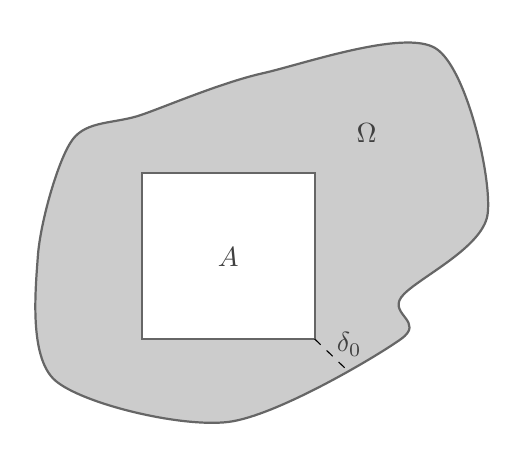
\begin{tikzpicture}
			 \begin{axis}[axis x line=none, axis y line=none]
				\addplot[mark=none, black!60, smooth cycle, thick, fill=gray!40] coordinates {(1,1) (2,0.5) (3,1.5) (3,2) (3.5,3) (3.2, 5) (2.2, 4.7) (1.5, 4.2) (1.1, 3.9) (0.9, 2.5)};
				\node[black!75] at (axis cs:2.8,3.75) [anchor=south] {$\Omega$};
				\addplot[mark=none, black!60, thick, fill=white!30] coordinates {(2.5,1.5) (2.5,3.5) (1.5,3.5) (1.5,1.5) (2.5,1.5)};
				\node[black!75] at (axis cs:2,2.25) [anchor=south] {$A$};
				\addplot[dashed] coordinates {(2.5,1.5) (2.7,1.1)};
				\node[black!75] at (axis cs:2.7,1.175) [anchor=south] {$\delta_{0}$};
			 \end{axis}
			\end{tikzpicture}
		\end{figure}
			
		Da $\supp(\phi_{\delta}) \subset B(0, \delta)$ nach \hyperref[bem:8.7ii]{8.7 ii)}
		\[ \Rightarrow \supp(g \ast \phi_{\delta} ) \subset A + B\left(0, \frac{\delta_{0}}{2}\right) \subset \Omega \text{ für } \delta < \frac{\delta_{0}}{2} \]
		(mit $A + B := \{ x + y : x \in A, y \in B\}$), denn $g \ast \phi_{\delta}(u) = \int \phi_{\delta}(u - v) g(v) dv \neq 0$ nur wenn $v \in A$ und $\| u - v \| < \delta$. \\
		Also $g \ast \phi_{\delta} \in C_{c}(\Omega)$. Zu zeigen: $g \ast \phi_{\delta} \in C^{\infty}(\Omega)$
		\[ D_{u}^{\alpha}(\phi_{\delta} \ast g)(u) = \int_{A} \left[ D_{u}^{\alpha} \phi_{\delta}(u - v) \right] \underbrace{g(v)}_{\text{beschränkt}} gv \]
		d.h. $\phi_{\delta} \ast g \in C	^{\infty}$; in einfachen Worten bedeutet das, dass $C_{\delta} \ast g$ alle guten Eigenschaften von $\phi$ $"$erbt$"$, auch wenn $g$ $"$schlecht$"$ ist. \\
		\[ \| f - \phi_{\delta} \ast g \|_{L^{p}} \leq \underbrace{\| f - g \|}_{\leq \epsilon} + \underbrace{\| g - \phi_{\delta} \ast g \|_{L^{p}}}_{\leq \epsilon} \text{ für } \epsilon \text{ klein genug nach } \hyperref[satz:8.8]{8.8} \]
	\end{beweis}
\end{kor}


\begin{bemerkung*}
	Es gilt:
	\begin{itemize}
		\item $\supp(f) \subset A, \supp(g) \subset B \quad \Rightarrow  \quad \supp(f + g) \subset A + B $
		\item $f \ast g = g \ast f$
	\end{itemize}	
\end{bemerkung*}


\begin{kor} \label{kor:8.10}
	Sei $\Omega \subseteq \MdR^{d}$ offen. Sei $f \in L^{p}(\Omega), p \in [1, \infty)$ mit $\int f(u) g(u) du = 0$ für alle $g \in C_{c}^{\infty}(\Omega)$. Dann ist $f = 0$.
	\begin{beweis}
		Zu $f \in L^{p}$ gibt es ein $g \in L^{p'}, \frac{1}{p} + \frac{1}{p'} = 1$ mit 
		\[ \| f \|_{L^{p}} = \int f(u) g(u) du, \quad \| g \|_{L^{p'}} = 1 \]
		Wähle $g(u) = |f(u)|^{p - 1} \left( sign(f(u)) \right) \cdot \| f \|_{L^{p}}^{\frac{1}{p} - 1}$. Dann ist
		\begin{align*}
			\| f \|_{L^{p}} & = \left( \int |f(u)|^{p} du \right)^{\frac{1}{p}} = \| f \|_{L^{p}}^{\frac{1}{p} - 1} \int |f(u)|^{p} du \\
			& = \int f(u) \underbrace{\frac{sign(f(u)) |f(u)|^{p - 1}}{\| f \|^{1 - \frac{1}{p}}}}_{=: g(u)} du \\
			& = \int f(u) g(u) du
		\end{align*}
		$\| g \|_{L^{p'}} = 1$ mit $\frac{1}{p} + \frac{1}{p'} = 1$. (sieh auch \hyperref[satz:8.1]{Beweis 8.1}) 
		\[ \| f \|_{L^{p}} = \int f(u) g(u) du = \int f(u) [g(u) - \phi(u)] du \text{ für alle } \phi \in C_{c}^{\infty}(\Omega), \quad \text{ denn } \int f(u) \phi(u) du = 0 \]
		Wähle nach \hyperref[kor:8.9]{8.9} ein $\phi \in C_{c}^{\infty}(\Omega)$ mit $\| g - \phi \|_{L^{p'}(\Omega)} < \frac{1}{2}$ \\ \\
		Also $\| f \|_{L^{p}} \underset{\text{Hölder}}{\leq} \| f \|_{L^{p}} \| f - \phi \|_{L^{p'}} < \frac{1}{2} \| f \|_{L^{p}}$, was einen Widerspruch zu $f \neq 0$ darstellt, demnach gilt $\| f \|_{L^{p}} = 0, f = 0$.
	\end{beweis}
\end{kor}



\newpage	
%!TEX root = Funktionalanalysis - Vorlesung.tex

\chapter*{Elemente der Operatortheorie} \addcontentsline{toc}{chapter}{Elemente der Operatortheorie} \setcounter{section}{8}



\section{Der Satz von Baire und der Satz von Banach-Steinhaus}



\begin{satz}[Satz von Baire] \label{satz:9.1-baire} \index{Baire}
	Sei $(M, d)$ ein vollständiger metrischer Raum und seien $(U_{n})_{n \geq 1}$ offen und dicht in $M$.
	\[ \text{Dann ist } \bigcap_{n \in \MdN} U_{n} \text{ dicht in } M. \]
\end{satz}

\begin{beweis}
    Wir definiere der Kürze halber $D \coloneqq \bigcap_{n \in \MdN} U_{n}$ und werden zeigen, dass zu jedem $x_{0} \in M$ und jedem $\epsilon > 0$ ein $x \in K(x_{0}, \epsilon) \cap D$ existiert. Für gegebenes $\epsilon > 0$
	\begin{itemize}
		\item ist $U_{1} \cap K(x_{0}, \epsilon)$ offen und nichtleer, da $U_{1}$ dicht ist. Also existiert ein $x_{1} \in U_{1}$ und $\epsilon_{1} > 0$ mit $\epsilon_{1} < \frac{1}{2} \epsilon$ so, dass $K( x_{1}, 2 \epsilon_{1}) \subset U_{1} \cap K(x_{0}, \epsilon)$
			\[ \Rightarrow \overline{K(x_{1}, \epsilon_{1})} \subseteq U_{1} \cap K(x_{0}, \epsilon) \]
		\item ist $U_{2} \cap K(x_{1}, \epsilon_{1})$  offen und nichtleer, da $U_{1}$ dicht ist. Also existiert ein $x_{2} \in U_{2}$ und ein $\epsilon_{2} < \frac{1}{2} \epsilon_{1}$ mit
			\[ \overline{K(x_{2}, \epsilon_{2})} \subset K(x_{2}, 2 \epsilon_{2}) \subset U_{2} \cap K(x_{1}, \epsilon_{1}) \subset U_{2} \cap U_{1} \cap K(x_{0}, \epsilon) \]
		\item Induktiv findet man Folgen $\epsilon_{n} > 0, x_{n}$ mit
			\begin{enumerate}[label=(\roman*\upshape)]
				\item $\epsilon_{n} < \frac{1}{2} \epsilon_{n - 1}$ und damit $\epsilon_{n} < \frac{1}{2^{n}} \epsilon$
				\label{satz:9.1-proof-ii}
				\item $\overline{K(x_{n}, \epsilon_{n})} \subset U_{n} \cap K(x_{n - 1}, \epsilon_{n - 1}) \subset \dotsc \subset U_{n} \cap \dotsc \cap U_{1} \cap K(x_{0}, \epsilon)$
			\end{enumerate}
	\end{itemize}
	Insbesondere für $n > N$:
	\[ d(x_{n}, x_{N}) \leq \sum_{j = N + 1}^{n} d(x_{j}, x_{j - 1}) \leq \sum_{j = N + 1}^{n} \epsilon_{n} \leq \left( \sum_{j = N + 1}^{\infty} \frac{1}{2^{j}} \right) \epsilon \]
	d.h. $(x_{n})$ ist eine Cauchy-Folge und da $M$ vollständig ist, existiert $\lim_{n \rightarrow \infty} x_{n} =: x$ in $M$. \\
	Mit \hyperref[satz:9.1-proof-ii]{ii)} gilt: $x_{n} \in \overline{K(x_{N}, \epsilon_{N})}$ für alle $n \geq N$
	\[ \Rightarrow x = \lim_{n \rightarrow \infty} x_{n} \in \overline{K(x_{N}, \epsilon_{N})} \subset U_{N} \cap \dotsc \cap U_{1} \cap K(x_{0}, \epsilon), ~ \forall N \in \MdN \]
	\[ \Rightarrow x \in \bigcap_{n = 1}^{\infty} U_{n} \cap K(x_{0}, \epsilon) = D \cap  K(x_{0}, \epsilon) \]
\end{beweis}


\begin{definition} \label{def:9.2}
	\begin{enumerate}[label=\alph*\upshape)]
		\label{def:9.2a}
		\item Eine Teilmenge $L$ eines metrischen Raums $M$ hei{\ss}t \begriff{nirgends dicht}, falls $\overline{L}$ keine inneren Punkte enthält.
		\label{def:9.2b}
		\item Eine Teilmenge $L$, die sich als Vereinigung von einer Folge von nirgends dichten Mengen $L_{n}$ darstellen lässt, d.h. $L = \bigcup_{n \in \MdN} L_{n}$ hei{\ss}t von \begriff{1. Kategorie}.
		\label{def:9.2c}
		\item $L$ hei{\ss}t von \begriff{2. Kategorie}, falls $L$ nicht von 1. Kategorie ist.
	\end{enumerate}
\end{definition}


\begin{bemerkung*}
	\begin{itemize}
		\item Ist $L$ nirgends dicht, dann ist $M \setminus \overline{L}$ dicht in $M$
		\item Ist $L$ nirgends dicht oder von Kategorie 1, dann ist $L$ $"$dünn$"$, $"$voller Löcher$"$.
	\end{itemize}	
\end{bemerkung*}


\begin{kor}[Kategoriensatz von Baire] \label{kor:9.3-KategoriensatzVonBaire}
	\begin{enumerate}[label=\alph*\upshape)]
		\item In einem vollständigen metrischen Raum $(M, d)$ liegt das Komplement einer Menge $L$ von 1. Kategorie stets dicht. Insbesondere:
		\item Ein vollständig metrischer Raum ist von 2. Kategorie
		\item Sei $(M, d)$ vollständig und $(M_{n})_{n \geq 1}$ eine Folge abgeschlossener Mengen mit $M = \bigcup_{n \in \MdN} M_{n}$. Dann enthält mindestens ein $M_{n}$ eine Kugel
	\end{enumerate}	
\end{kor}

\begin{beweis}
	$L = \bigcup_{n \in \MdN} L_{n}$, $L_{n}$ nirgends dicht. \\
	Damit gilt $L^{c} = \left( \bigcup_{n \in \MdN} L_{n} \right)^{c} = \bigcap_{n \in \MdN} L_{n}^{c} \supset \bigcap_{n \in \MdN} \overline{L_{n}}^{c}$, mit $\overline{L_{n}}^{c}$ offen. \\
	Da $L_{n}$ nirgends dicht ist, ist daher $\overline{L_{n}}^{c}$ dicht in $M$ \\
	Nach \hyperref[satz:9.1-baire]{9.1} ist auch $\bigcap_{n \in \MdN} \overline{L_{n}}^{c}$ dicht in $M$ und da $\bigcap_{n \in \MdN} \overline{L_{n}}^{c} \subset L^{c}$, ist auch $L^{c}$  dicht in $M$. \\ \\
	$a) \Rightarrow b) \Rightarrow c)$ nach Definition.
\end{beweis}


\begin{satz}
	$E = \{ x \in C[0, 1]:$ $x$ ist in keinem Punkt von $[0, 1]$ differenzierbar$\}$ ist dicht in $(C[0, 1], \|\cdot\|_{\infty})$. \\
	Insbesondere:
 		\begin{itemize}
			\item $E \neq \emptyset$
			\item $C^{1}[0, 1]$ ist von 1. Kategorie in $C[0, 1]$, also liegt $C[0, 1] \setminus C^{1}[0, 1]$ dicht in $C[0, 1]$.
		\end{itemize}
\end{satz}

\begin{beweis}
	Betrachte die Menge
	\[ E_{n} = \left\{ x \in C[0, 1]: \sup_{0 < |h| \leq \frac{1}{n}} \left| \frac{x(t + h) - x(t)}{h} \right| > n, \text{ für alle } t \in [0, 1] \right\}, \]
	dann ist $\bigcap_{n \geq 1} E_{n} \subset E$. 
	
	\newpage % temporarily for optics
	
	Damit wir den \hyperref[satz:9.1-baire]{Satz von Baire} anwenden können, müssen wir zeigen 
	\begin{enumerate}[label=\roman*\upshape)]
		\item $E_{n}$ sind offen in $C[0, 1]$ für alle $n$
		\item $E_{n}$ sind dicht in $C[0, 1]$ für alle $n$
	\end{enumerate}
	und erhalten dann, dass $\bigcap_{n \in \MdN} E_{n}$ und damit auch die Menge $E$ dicht in $C[0, 1]$ ist. \\
	\begin{enumerate}[label=\roman*\upshape)]
		\item Sei $n \in \MdN$ und $x \in E_{n}$ fest. \\
			Zu jedem $t \in [0, 1]$ wähle $\delta_{t}$ definiert durch: $\sup_{0 < |h| \leq \frac{1}{n}} \left| \frac{x(t + h) - x(t)}{h} \right| = n + 2 \delta_{t}$
			\[ \Rightarrow \left| \frac{x(t + h_{t}) - x(t)}{h_{t}} \right| > n + \delta_{t} \text{ für } 0 < |h_{t}| \leq \frac{1}{n} \]
			Da $x$ stetig ist, gibt es zu $t$ eine offene Umgebung $U_{t}$ mit
			\[ \left| \frac{x(s + h_{t}) - x(s)}{h_{t}} \right| > n + \delta_{t} \text{ für } s \in U_{t}, \quad 0 < |h_{t}| \leq \frac{1}{n} \]
			Da $[0, 1]$ kompakt und $[0, 1] = \bigcup_{t \in [0, 1]} U_{t}$ gibt es endlich viele $U_{t_{1}}, \dotsc, U_{t_{n}}$ mit 
				\[ [0, 1] \subset U_{t_{1}} \cup \dotsc \cup U_{t_{n}} \]
			Setze $\delta \coloneqq \min \{ \delta_{t_{1}}, \dotsc, \delta_{t_{1}} \} > 0$, $h \coloneqq \min \{ h_{t_{1}}, \dotsc, h_{t_{n}} \}$ und wähle ein $\epsilon$ mit $0 < \epsilon < \frac{1}{2} h \delta$. Zu zeigen bleibt $K(x, \epsilon) \subset E_{n}$: \\ 
			Sei $y \in C[0, 1]$ mit $\| x - y \|_{\infty} < \epsilon$. Zu $t \in [0, 1]$ wähle $i \in \{ 1, \dotsc, n \}$ mit $t \in U_{i}$. Dann:
			\begin{align*}
				\left| \frac{y(t + h_{t_{i}}) - y(t)}{h_{t_{i}}} \right| & \overset{\triangle-\text{Ungl.}}{\geq} \left| \frac{x(t + h_{t_{i}}) - x(t)}{h_{t_{i}}} \right| - 2 \frac{\| x - y \|_{\infty}}{|h_{t_{i}}|} \\
				& \overset{t \in U_{t_{i}}}{>} n + \delta - 2 \frac{\epsilon}{n} \\
				& > n \quad \text{nach Wahl von } \epsilon
			\end{align*}
			$\Rightarrow x \in E_{n}, K(x, \epsilon) \subseteq E_{n} \Rightarrow A_{n}$ offen, $n \in \MdN$.
		\item Wir wollen noch zeigen, dass $U_{n}$ dicht in $C[0, 1]$ ist. \\
			Sei $V \subset C[0, 1]$ offen, $V \neq \emptyset$. Nach dem Approximationssatz von Weierstra{\ss} gibt es ein Polynom $p$ mit $p \in V, \epsilon > 0: \| x - p \|_{\infty} \leq \epsilon \Rightarrow x \in V$. \\
			Sei weiter $y_{m}$ eine Sägezahnfunktion mit $y_{m}: [0, 1] \rightarrow [0, \epsilon]$ und der Steigung $\pm m$.
			Dann ist $x \coloneqq p + {m} \in K(p, \epsilon)$. \\
			Wähle zu $n$ die Zahl $m \in \MdN$ so, dass $m > n + \| p \|_{\infty}$. \\
			Für $t \in [0, 1], 0 < | n | \leq \frac{1}{n}$ gilt:
			\[ \left| \frac{x_{m}(t + h) - x(t)}{h} \right| \overset{\triangle-\text{Ungl.}}{\geq} \left| \frac{y_{m}(t + h) - y(t)}{h} \right| - \underbrace{\left| \frac{p(t + h) _ p(t)}{h} \right|}_{\leq{\| p' \|_{\infty}} \text{nach MWS}}  \]
			\[ \Rightarrow \sup_{0 < |h| \leq \frac{1}{n}} \left| \frac{x_{m}(t + h) - x_{m}(t)}{h} \right| \geq m - \| p' \|_{\infty} \overset{\text{nach Wahl}}{\underset{\text{von }m}{\geq}} n \] \\
			Damit ist $x_{m} \in E_{n}$ und sogar $x_{m} \in E_{n} \cap V$ \\ \\
			$\Rightarrow E_{n} \cap V \neq \emptyset \quad \Rightarrow E_{n} \text{ dicht.}$
	\end{enumerate}	
\end{beweis}


\begin{satz}[Banach-Steinhaus] \label{satz:9.5-Banach-Steinhaus} \index{Banach-Steinhaus}
	Sei $X$ ein Banachraum, $Y$ ein normierter Raum, $I$ eine Indexmenge und $(T_{i})_{i \geq 1} \in B(X, Y)$.
	Falls:
	\[ \sup_{i \in I} \| T_{i} x \| = c(x) < \infty, \quad \forall x \in X \]
	dann ist auch
	\[ \sup_{i \in I} \| T_{i} \| = \sup_{i \in I} \sup_{\| x \| \leq 1} \| T_{i} x \| < \infty. \]
\end{satz}

\begin{beweis}
	Betrachte die Menge $E_{n} \coloneqq \{ x \in X: \sup \| T_{i} x \| \leq n\}$. Dann ist $E_{n}$ abgeschlossen, denn $E_{n} = \bigcap_{i \in \MdN} \{ x \in X: \| T_{i} x \| \leq n \}$. Außerdem ist $E_{n}$ symmetrisch, d.h. $x \in E_{n} \gdw -x \in E_{n}$ und konvex, denn für $x_{1}, x_{2} \in E_{n}$ gilt
		\[ \sup \| T_{i} \left( \frac{1}{2} x_{1} + \frac{1}{2} x_{2} \right) \| \leq \frac{1}{2} \sup \| T_{i} x_{1} \| + \frac{1}{2} \sup \| T_{i} x_{2} \| \leq n \quad \text{also } \frac{1}{2} x_{1} + \frac{1}{2} x_{2} \in E_{n} \]
		Es gilt $X = \sum_{n = 1}^{\infty} E_{n}$, nach \hyperref[satz:9.1-baire]{Baire} existiert dann ein $N \in \MdN, x \in E_{N}, \epsilon > 0$ mit $K(x, \epsilon) \subset E_{N} \Rightarrow K(-x, \epsilon) \subseteq E_{n}$ \\
		Sei $z \in X: \| z \| < \epsilon$. $z = \frac{1}{2} (x + z) + \frac{1}{2} (z - x) \in \frac{1}{2} E_{N} + \frac{1}{2} E_{N} \subseteq E_{N}$. 
		\[ \Rightarrow \sup_{i \in \MdN} \sup_{\| z \| \leq 1} \| T_{i} z \| = \sup_{i \in \MdN} \sup_{\| z \| < \epsilon} \| T_{i} \frac{z}{\epsilon} \| \leq \sup_{i \in \MdN} \sup_{z \in E_{N}} \frac{1}{\epsilon} \| T_{i} z \| \leq \frac{N}{\epsilon} \]	
\end{beweis}


\begin{bemerkung}  \label{bem:9.6}
	\begin{enumerate}[label=\alph*\upshape)]
		\item Der \hyperref[satz:9.5-Banach-Steinhaus]{Satz von Banach-Steinhaus} ist nicht konstruktiv d.h. aus $c(X)$ kann man $\sup_{i \in I} \| T_{i} \|$ nicht herleiten.
		\item Die Vollständigkeit von $X$ ist notwendig.
	\end{enumerate}	
\end{bemerkung}


\begin{beispiel*}
$F \coloneqq \{ (x_{n})_{n}: x_{n} = 0$ für alle, bis auf endlich viele $n \}$ mit $\| \cdot \|_{\infty}$ und betrachte $T_{k} (x_{n})_{n} = k x_{k}$. \\ 
	Dann gilt $\| T_{k} \| = k$ und $\sup_{k \in \MdN} \| T_{k} \| = \infty$, aber 
	\[ \sup_{k \in \MdN} \| T_{k} (x_{n})_{n} \| = \sup_{k \in \MdN} \| k x_{k} \| < \infty, \]
	da das Supremum nur über endlich viele Werte genommen wird.
\end{beispiel*}


\begin{kor} \label{kor:9.7}
	Sei $X$ ein Banachraum, $Y$ ein normierter Raum und $(T_{n})_{n \geq 1} \subset B(X, Y)$ derart, dass
	\[ \lim_{n \rightarrow \infty} T_{n} x =: y \text{ existiert für alle } x \in X \]
	Dann ist $T x \coloneqq y_{x}$ linear und $T \in B(X, Y)$.
	
	\newpage % todo temporarily for optics
	
	\begin{beweis}
		Da sowohl der Limes als auch $T_{n}$ für alle $n \in \MdN$ jeweils linear sind, ist $T$  linear. \\
		Insbesondere ist $(T_{n} x)_{n \geq 1}$ beschränkt; mit \hyperref[satz:9.5-Banach-Steinhaus]{Banach-Steinhaus} ist also auch $ \sup_{n \in \MdN} \| T_{n} \| < \infty$. \\
		\[ \| T x \| = \lim_{n \rightarrow \infty} \| T_{n} x \| \leq \sup_{n \in \MdN} \|T_{n} \| \cdot \|x \| \]
		\[ \Rightarrow T \in B(X, Y) \text{ mit } \| T \| \leq \sup_{n \in \MdN} \| T_{n} \|\]
	\end{beweis}
	Frage: $T_{n} \xrightarrow[n \rightarrow \infty]{} T$ in $B(X, Y)$? Nein, nicht im Allgemeinen! \\
\end{kor} 

\begin{beispiel*}
	$X = Y = \ell^{p}$, $T_{k} (x_{n})_{n} = (x_{1}, \dotsc, x_{k}, 0, \dotsc)$
	\[ \| T_{k} (x_{n})_{n} - I (x_{n})_{n} \|_{\ell^{p}} \left( \sum_{n = k + 1}^{\infty} | x_{n} |^{p} \right)^{\frac{1}{p}} \xrightarrow[k \rightarrow \infty]{} 0 \]
	Aber
		\[ \| T_{k} - I \| \geq \|(T_{k} - I)\underbrace{(0, \dotsc, 0, 1, 0, \dotsc)	}_{1 \text{ an } k+1-\text{ter Stelle}} \|_{\ell^{p}} = 1 \not\xrightarrow[ ~ ]{ } 0 \]
	D.h. punktweise Konvergenz impliziert keine Konvergenz bezüglich der Operatornorm.
\end{beispiel*}



\newpage	
\subsection*{10 - offenen Abbildung}

	\begin{karte}{Offene Abbildung}
			Eine Abbildung zwischen metrischen Räumen heißt \begriff{offen}, wenn offene Mengen auf offene Mengen abgebildet werden.
	\end{karte}
	
	\begin{karte}{Äquivalenzen zu offenem Operator}
				Seien $X, Y$ normierte Räume und $T: X \rightarrow Y$ ein linearer Operator, dann sind äquivalent:
		\begin{enumerate}[label=\alph*\upshape)]
			\item $T$ ist offen
			\item $\exists \epsilon > 0: K_{Y}(0, \epsilon) \subset T(K_{X}(0, 1))$
		\end{enumerate}
	\end{karte}
	
	\begin{karte}{Satz von der offenen Abbildung}
		Seien $X, Y$ Banachräume und $T \in B(X, Y)$, dann gilt:
		\[ T \text{ surjektiv} \gdw T \text{ offen} \]
	\end{karte}

	\begin{karte}{Bijektiver beschränkter Operator}	
		Seien $X, Y$ Banachräume und $T \in B(X, Y)$ bijektv, dann ist $T^{-1} \in B(Y, X)$	
	\end{karte}

	\begin{karte}{Beschränkte Einbettung zwischen Banachräumen}	
		Sei $X$	ein Vektorraum der sowohl mit $\| \cdot \|$ als auch mit $\vertiii{\cdot}$ ein Banachraum ist. Gilt 
		\[ \exists c > 0: \| x \| \leq c \cdot \vertiii{x}, ~ \forall x \in X, \]
		dann sind die Normen äquivalent, d.h. $\exists \hat{c} $ mit 
		\[ \hat{c} \cdot \vertiii{x} \leq \| x \| ~ \forall x \in X \leq c \cdot \vertiii{x} \]
	\end{karte}
%!TEX root = Funktionalanalysis - Vorlesung.tex

\section{Projektionen}



\begin{definition} \label{def:11.1-Projektion}
	Sei $X$ ein Banachraum. $P \colon X \rightarrow X$ hei{\ss}t \begriff{Projektion}, wenn $P$ linear und $P^{2} = P$ ist.
\end{definition}

Die Frage die wir uns dabei stellen sollten, lautet: wann ist $P$ beschränkt?

\begin{beispiel}
	\begin{enumerate}[label=\alph*\upshape)]
		\item $X = L^{p}(\MdR)$, $\Omega \subset \MdR: $ $\mu(\Omega) > 0$, $\mu(\MdR \setminus \Omega) > 0$
			\[ P f \coloneqq \1_{\Omega} f ~ \Rightarrow ~ P^{2} f = \1_{\Omega}^{2} f = \1_{\Omega} f = P f \]
			$\| P f \|_{L^{p}} = \left( \int | \1_{\Omega} f |^{p} d\mu \right)^{\frac{1}{p}} = \left( \int_{\Omega} | f |^{p} d\mu \right)^{\frac{1}{p}} \leq \| f \|_{L^{p}}$ $\Rightarrow P$ ist beschränkt.
		\item $X = L^{p}[0, 1]^{2},$ mit $1 \leq p < \infty$
			\[ P f(x, y) \coloneqq \int_{0}^{1} f(s, y) ds ~ \Rightarrow ~ P^{2} f (x, y) = \int_{0}^{1} \int_{0}^{1} f(s, y) ds dt = \int_{0}^{1} f(s, y) ds = P f(x, y) \]
			\begin{align*}
				\| P f \|_{L^{p}} & = \left( \int_{0}^{1} \int_{0}^{1} \left| \int_{0}^{1} f(s, y) ds \right|^{p} dy dx \right)^{\frac{1}{p}} \\
				& \overset{\triangle-\text{Ungl.}}{\leq} \left( \int_{0}^{1} \left( \int_{0}^{1} |f(s, y)| ds \right)^{p} dy \right)^{\frac{1}{p}} \\
				& \underset{()^{p} \text{ konvex!}}{\overset{\text{Jensen}}{\leq}}\left( \int_{0}^{1} \int_{0}^{1} |f(s, y)|^{p} ds dy \right)^{\frac{1}{p}} \\
				& = \| f \|_{L^{p}}
			\end{align*}
	\end{enumerate}
\end{beispiel}


\begin{bemerkung}
	Sei $X$ ein Vektorraum, $M \subset X$ ein Untervektorraum. Es gibt nach dem Basisergänzungssatz eine lineare Projektion $P \colon X \rightarrow X,$ $P(X) = M$	
\end{bemerkung}

\begin{beweis}
	Sei $(b_{i})_{i \in I}$ eine Basis von $M$ und $(b_{j})_{j \in J}$ von $X$, mit $I \subset J$. \\
	Nun existiert ein $(\alpha_{j}(x))_{j}$:
	\[ x = \sum_{j \in J} \alpha_{j}(x) b_{j} \text{ mit } \alpha_{j}(x) = 0 \text{ für fast alle } j \in J. \]
	$P(x) \coloneqq \sum_{i \in I} \alpha_{i}(x) b_{i}$.
\end{beweis}


\begin{erinnerung}
	Sind $X, Y$ Banachräume, dann ist auch $X \oplus Y$ ein Banachraum mit $\| (x, y) \|_{X \bigoplus Y} = \| x \|_{X} + \| y \|_{Y}$ $\forall x \in X, y \in Y$
\end{erinnerung}


\begin{satz} \label{satz:11.4}
	Sei $X$ ein Banachraum, $M \subset X$ ein abgeschlossener Untervektorraum. Dann sind folgende Aussagen äquivalent:
	\begin{enumerate}[label=\alph*\upshape)]
		\item Es gibt eine stetige Projektion $P \colon X \rightarrow X$ mit $P(X) = M$
		\item Es gibt einen abgeschlossenen Untervektorraum $N \subset X: X = M \oplus N$.
		\item Es gibt einen abgeschlossenen Untervekottraum $N \subset X$ und $J: M \oplus N \rightarrow X,$ $J(x, y) = x + y$ ist ein Isomorphismus, insbesondere $\exists c > 0$ $\forall x \in M, y \in N:$ $c \left( \|x \| + \|y \| \right) \leq \|x + y \| \leq \|x \| + \| y \| $
	\end{enumerate}
\end{satz}

\begin{beweis}
	$a) \Rightarrow b)$ Definiere $N = (I - P)(X)$. Dann gilt
		\[ X = P(X) + (I - P)(X) \text{ und } P(X) \cap (I - P)(X) = \{ 0 \} \]
		$N$ ist abgeschlossen, denn $N = \kernn{P} = P^{-1}\{ 0 \}$ und $P$ ist stetig.	\\ \\
	$b) \Rightarrow c)$ Sei $N$ wie in $b)$. $J: M \oplus N \rightarrow X,$ $J(x, y) = x + y$. Dann gilt:
		\begin{align*}
			\| x + y \| & = \| J(x, y) \| \quad \forall x \in M, y \in N \\
						& \leq \| x \| + \| y \| \\
						& = \| (x, y) \|_{M \oplus N}
		\end{align*}
		Au{\ss}erdem ist $J$ bijektiv, da $X = M \oplus N$
		$\xRightarrow[]{\ref{kor:10.5}} J^{-1} stetig,$ $\exists \hat{c} > 0: \forall x \in M, y \in N$:
		\[ \| x + y \| - \| (x, y) \| = \| J^{-1}(x + y) \| \leq \hat{c} \| x + y \| \]

	$c) \Rightarrow a)$ Definiere $\hat{P} \colon M \oplus N \rightarrow M \oplus N,$ $\hat{P}(x, y) = (x, 0)$
		\[ \Rightarrow \hat{P}(M \oplus N) = M \oplus \{ 0 \}. \text{ Setze } P = J \hat{P} J^{-1} \quad (P \text{ ist Projektion!}) \]
		$P(X) = M$, denn $P(X) = J \hat{P}(M \oplus N) = J (M \oplus \{ 0 \}) = M$
\end{beweis}


\begin{vereinbarung}
	$M$ hei{\ss}t komplementierter Raum, $N = \kernn(P)$ Komplementärraum.
\end{vereinbarung}


\begin{beispiel*}
	\begin{enumerate}[label=\alph*\upshape)]
		\item $X = L^{p}(\MdR)$ $\Omega \subseteq \MdR,$ $P f = \1_{\Omega} f$
			\begin{align*}
				M & = P(X) = \{ f \in L^{p}(\MdR): f = 0 \text{ fast überall auf } \Omega^{c} \} \\
				N & = \kernn(f) = \{ f \in L^{p}(\MdR): f = 0 \text{ fast überall auf } \Omega \}
			\end{align*} 
		\item $X = L^{p}([0, 1]^{2})$ $P f(x, y) = \int_{0}^{1} f(s, y) ds$
			\begin{align*}
				M & = \{ f \in L^{p}([0, 1]^{2}), f \text{ konstant in 1. Komponente} \} \\
				N & = \{ f \in L^{p}([0, 1]^{2}): \int_{0}^{1} f(s, y) ds = 0 \text{ fast überall, } y \in [0, 1] \}
			\end{align*}
	\end{enumerate}
	Sowohl in $a)$ als auch in $b)$ gilt $X = M \oplus N$, da $P$ in beiden Fällen stetig ist.
\end{beispiel*}



\newpage
\subsection*{12 - Abg. Operatoren}

	\begin{karte}{Operatorfortsetzung}
		Sei $X$ ein Banachraum, $D(A)$ ein dichter Untervektorraum und $A: D(A) \rightarrow X$ linear
	
		Gilt $\| A x \| \leq c \| x \|$ $\forall x \in D(A)$, so lässt sich $A$ zu einem beschränkten Operator fortsetzen $A \in B(X)$	
	\end{karte}
	


	\begin{karte}{Graphennorm}
		Auf $D(A)$ definieren wir die \begriff{Graphennorm}
		\[ \| x \|_{A} \coloneqq \|x \| + \| A \| \quad \forall x \in D \]
		Insbesondere: $A: (D(A), \| \cdot \|_{A}) \rightarrow X$ stetig, denn 
		\[ \| X \| \leq \|x \| + \| A x \| = \| x \|_{A} \]
	\end{karte}


	\begin{karte}{Abgeschlossener Operator}
		Es sind äquivalent
		\begin{enumerate}[label=\alph*\upshape)]
			\item $\left( D(A), \| \cdot \|_{A} \right)$ ist ein Banachraum
			\item $\ograph(A) = \{ (x, A x): x \in D(A) \} \subset X \times X$ ist abgeschlossen
			\item Wenn $(x_{n})_{n} \subset D(A): \begin{cases}
			x_{n} \xrightarrow[]{n \rightarrow \infty} x & \text{ in } X \\ A x_{n} \xrightarrow[]{n \rightarrow \infty} y & \text{ in } X \end{cases}$, $ $ so ist $x \in D(A), A x = y$
		\end{enumerate}
	
		$A$ hei{\ss}t abgeschlossen, wenn $a) - c)$ aus \hyperref[satz:12.3]{12.3} erfüllt sind	
	\end{karte}


	\begin{karte}{Abgeschlossener vs. stetiger Operator}
		\begin{align*}
			A \text{ stetig: } & x_{n} \xrightarrow[]{n \rightarrow \infty} x \Rightarrow Ax_{} \xrightarrow[]{n \rightarrow \infty} y, Ax = y \\
			A \text{ abgeschlossen: } & x_{n} \xrightarrow[]{n \rightarrow \infty} x, A x_{n} \xrightarrow[]{n \rightarrow \infty} y \Rightarrow Ax = y
		\end{align*}
	\end{karte}


	\begin{karte}{Satz vom abgeschlossenen Graphen}
		Ist $A$ abgeschlossen und $D(A) = X$, so ist $A$ stetig auf $X$.
	\end{karte}

%!TEX root = Funktionalanalysis - Vorlesung.tex

\section{Spektrum und Resolvente}



Sei $Y \supset D(A) \rightarrow X$ linear, $\lambda \in \MdC$.
	\[ (\lambda I - A) x = y \quad (*) \label{eq:13.0-lineareGleichung} \]
Problem: Gegeben $y \in X$ finde $x \in D(A)$ so, dass \hyperref[eq:13.0-lineareGleichung]{$(*)$} erfüllt ist.
Formel: $x = (\lambda I - A)^{-1}$ ist Lösung, falls $(\lambda I - A)^{-1}$ existiert.


\begin{definition}
	Sei $X$ ein Banachraum über $\MdC$, $X \supset D(A) \rightarrow X$ linear und abgeschlossen.
	\begin{enumerate}[label=\alph*\upshape)]
		\item $\lambda \in \MdC$ gehört zur \begriff{Resolventenmenge} von $A$, $\lambda \in \rho(A)$, falls
			\[ \lambda I - A : D(A) \rightarrow X \text{ bijektiv, d.h. } (\lambda I - A)^{-1}: X \rightarrow D(A) \text{ linear} \]
		\item $\sigma(A) = \MdC \setminus \rho(A)$ hei{\ss}t \begriff{Spektrum} von $A$
		\item $\lambda \in \rho(A) \rightarrow R(\lambda, A) = (\lambda - A)^{-1}$ hei{\ss}t \begriff{Resolventenfunktion} von A
	\end{enumerate}	
\end{definition}


\begin{erinnerung}
	$A$ abgeschlossen $\gdw$ ... todo % todo missing sth at 13.1: add rep	
\end{erinnerung}


\begin{bemerkung}
	$A$ ist abgeschlossen, falls $\lambda \in \rho(A)$, so ist $R(\lambda, A) \in B(X)$ und $R(\lambda, A): X \rightarrow A): X \rightarrow (D(A), \| \cdot \|_{A})$ ein Isomorphismus.
\end{bemerkung}

\begin{beweis}
	$(\lambda - A): (D(A), \| \cdot \|_{A}) \rightarrow A$ ist bijektiv und stetig, denn $\|(\lambda - A)x \| \leq \max(1, |\lambda|) (\|x\| + \|Ax\|) = c \| x \|_{A}$ \\
	Nach dem \hyperref[satz:10.3-offeneAbbildung]{Satz der offenen Abbildung} ist
		\[ R(\lambda, A): X \rightarrow (D(A), \| \cdot \|_{A}) \]
	ein Isomorphismus: $X \xrightarrow[]{R(\lambda, A)} (D(A), \| \cdot \|_{A}) \subset X$. Also $R(\lambda, A) \in B(X)$.
\end{beweis}


\begin{beispiel}
	\begin{enumerate}[label=\alph*\upshape)]
		\item $X = \MdC^{d}, A \in B(X) \equalhat M(d, d)$
			\[ \sigma(A) = \{ \lambda \text{ Eigenwerte von A} \} \]
		\item Sei $\alpha_{n} \in \MdC,$ $X = \ell^{p}, 1 \leq p < \infty, A(x_{n}) = (\alpha_{n} x_{n}),$ $(x_{n}) \in D(A) = \{ (x_{n}): \sum_{n \geq 1} | \alpha_{n} x_{n} |^{p} < \infty \}$. \\
			Falls $(\alpha_{n})$ beschränkt ist, dann ist $D(A) = \ell^{p}, A \in B(\ell^{p})$. \\
			Für allgemeine $(\alpha_{n}) \subset \MdC$ ist $A$ nur abgeschlossen (Übung). \\
			Dann ist $\sigma(A) = \overline{\{ \alpha_{n}, n \in \MdN \}}^{c}$, da $A(e_{n}) - \alpha_{n}(e_{n}) = 0$ ($e_{n}$ n-ter Einheitsvektor) \\ \\
			Beweis: $(\lambda I - A)(x_{n}) = ((\lambda - \alpha) x_{n})$ \\
			Formal: $(\lambda I - A)^{-1}(x_{n}) = ((\lambda - \alpha_{n})^{-1}x_{n})$
			\begin{align*}
				\| (\lambda - A)^{-1} \| \underset{\text{Übung}}{=} \sup_{n} | \lambda - \alpha_{n} |^{n} = \frac{1}{d(\lambda, \overline{(\alpha_{n})})} < \infty & \gdw d(\lambda, \overline{(\alpha_{n})}) > 0 \\
				& \gdw \lambda \notin \overline{(\alpha_{n})}
			\end{align*}
			$\Rightarrow \lambda \in \rho(A) \gdw \lambda \in \overline{\{\alpha_{n}\}}, $ $ $ $ \lambda \in \sigma(A) \gdw \lambda \in \overline{(\alpha_{n})}$ \\ \\
			\textbf{Folgerung:} Jede abgeschlossene Menge $S \subseteq \MdC$ kann das	 Spektrum eines abgeschlossenen Operators sein. Insbesondere: $\sigma(A)$ kann überabzählbar sein. Das Spektrum $\sigma(A)$ besteht im Allgemeinen nicht nur aus Eigenwerten.
			\begin{beweis}
				Gegeben $M \subset \MdC$ abgeschlossen, wähle dichte Folge $\alpha_{n} \in M$, d.h. $\{ \alpha_{n} \} = M$ \\
				Wähle $X = \ell^{p},$ $A(x_{n}) = (\alpha_{n} x_{n}),$ $\sigma(A) = \overline{\{ \alpha_{n} \}} = M$.
			\end{beweis}
			Falls $\lambda \in \overline{\{ \lambda_{n} \}} \setminus \{ \lambda_{n} \}$ dann ist $\lambda$ kein Eigenwert von $A$.
		\item Sei $X = \ell^{p}$, $e_{n}$ Einheitsvektoren.
			\[ A (e_{1}) = 0, A (e_{n}) = e_{n - 1}, n > 1 \Rightarrow A(x_{1}, x_{2}, x_{3}, \dotsc) = (x_{2}, x_{2}, x_{3}, \dotsc) \]
			\[ B (e_{n}) = e_{n + 1}, n \geq 1 \Rightarrow B(x_{1}, x_{2}, x_{3}, \dotsc) = (0, x_{1}, x_{2}, x_{3}, \dotsc) \]
			Übung: $\sigma(A) = \sigma(B) = \{ \lambda : | \lambda | \leq 1 \}$
	\end{enumerate}
\end{beispiel}


\begin{satz}[Resolventendarstellung] \label{satz:13.4-Resolventendarstellung}
	Sei $X \supset D(A) \xrightarrow[]{A} X$ abgeschlossen, $X$ ein Banachraum. \\
	Für $\lambda:{0} \in \rho(A)$ und $\lambda \in \MdC$ mit $|\lambda - \lambda_{0}| < \frac{1}{\| R(\lambda_{0}, A) \|}$ ist auch \\
		\[ \lambda \in \rho(A) \text{ und } R(\lambda, A) = \sum_{n \geq 0} (\lambda_{0} - \lambda)^{n} R(\lambda_{0}, A)^{n + 1}. \] \\
	Insbesondere ist $\rho(A)$ offen und $\sigma(A)$ abgeschlossen.
\end{satz}

\begin{beweis}
	\begin{align*}
		 (\lambda - A) = (\lambda_{0} + \lambda) + (\lambda_{0} - A) & = (\lambda_{0} - A)\left[I - (\lambda_{0} - \lambda) R(\lambda_{0}, A)\right] \\
		 & = (\lambda_{0} - A)(I - S) \quad \text{ mit } S = (\lambda_{0} - \lambda)R(\lambda_{0}, A)
	\end{align*}	
	\[ \Rightarrow \| S \| \leq | \lambda_{0} - \lambda| \| R(\lambda_{0}, A) \| \overset{Vor.}{<} 1. \text{ Nach dem Satz über die Neumannsche Reihe: } (I - S)^{-1} = \sum_{n \geq 0} S^{n} \]
	Dann ist $(\lambda - A)$ ein Produkt von invertierbaren Operatoren $(\lambda_{0} - A)$ und $(I - S)$, d.h. 
	\begin{align*}
		(\lambda - A)^{-1} & = (I - S)^{-1}(\lambda_{0} - A)^{-1} \\
			& = \sum_{n \geq 0} \underbrace{(\lambda_{0} - \lambda)^{n}R(\lambda_{0}, A)^{n}}_{= S^{n}} R(\lambda_{0}, A) \\
			& = \sum_{n \geq 0} (\lambda_{0} - \lambda)^{n} R(\lambda_{0}, A)^{n + 1}
	\end{align*} 
\end{beweis}


\begin{satz}[Resolventengleichung] \index{Resolventengleichung}
	Sei $A$ ein abgeschlossener Operator auf $X$. Für $\lambda, \mu \in \rho(A)$ gilt:
		\[ R(\lambda, A) - R(\mu, A) = (\mu - \lambda) R(\lambda, A) R(\mu, A) \]
	Insbesondere ist $\lambda \in \rho(A) \rightarrow R(\lambda, A) \in B(X)$ eine komplex differenzierbare Abbildung und 
		\[ \frac{d}{d \lambda} R(\lambda, A) = - R(\lambda, A)^{2} \]
\end{satz}

\begin{beweis}
	\begin{align*}
		R( \lambda, A) - R( \mu, A) & = R( \lambda, A) \left[ I - (\lambda - A) R(\mu, A) \right]	\\
			& = R( \lambda, A) \left[ \mu - A - \lambda + A \right] R(\mu, A)
	\end{align*}
	$\Rightarrow$ Behauptung. (Idee: $\frac{1}{\lambda - a} - \frac{1}{\mu - a} = \frac{\mu - \lambda}{(\lambda - a)(\mu - a)}$)
	\begin{align*}
		\frac{d}{dx} R(\lambda, A) & = \lim_{\mu \rightarrow \lambda} \frac{R(\mu, A) - R(\lambda, A)}{\mu - \lambda} \\
				& \overset{s.o.}{=} \lim_{\mu \rightarrow \lambda} \left[ - R( \lambda, A) R(\mu, A) \right] \\
				& = - R(\lambda, A)^{2}, \text{ denn } \lambda \in \rho(A) \rightarrow R(\lambda, A) \in B(X) \text{ ist stetig als Potenzreihe.} 		
	\end{align*}
\end{beweis}


\begin{satz}
	Falls $A \in B(X)$, dann ist $\sigma(A)$ nichtleer und kompakt mit $\sigma(A) \subset \{ \lambda : |\lambda| \leq \| A \| \}$ \\
	\[ \text{Für } \lambda > \| A \| \text{ gilt: } R(\lambda, A) = \sum_{n \geq 0} \lambda^{-n-1} A^{n} \]
\end{satz}

\begin{beweis}
	Für $| \lambda | > \| A \|$ gilt: $\lambda - A = \lambda [I - S]$ mit $S = \frac{A}{\lambda}, \| S \| \leq \frac{\| A \|}{| \lambda |} < 1$ nach Voraussetzung. \\
	Nach Neumann: 
	\begin{align*}
		(I - S)^{-1} & = \sum_{n = 0}^{\infty} S^{n} (\lambda - A)^{-1} \\
			& = \lambda^{-1} [I - S]^{-1} \\
			& = \lambda^{-1} \sum_{n = 0}^{\infty} \left( \frac{A}{\lambda} \right)^{n} \\
			& = \sum_{n = 0}^{\infty} \lambda^{-n-1} A^{n}
	\end{align*}
	Also: $\sigma(A) \subset \{ \lambda: |\lambda| \leq \|A\| \}, \sigma(A)$ beschränkt, abgeschlossen $\Rightarrow \sigma(A)$ kompakt. \\
	Wir müssen noch zeigen, dass $\sigma(A) \neq \emptyset$. \\
	Nach \hyperref[bem:8.7]{Bemerkung 8.7} gibt es in jedem Banachraum $X$ $x \in X, x' \in X'$ mit $x'(x) \neq 0$ $(*)$ \label{eq:13.6.5-DualAbbildungAuf0} \\
	Indirekter Beweis für $\sigma(A) \neq \emptyset$. \\
	Annahme $\sigma(A) = \emptyset$ bzw. $\rho(A) = \MdC$ \\
	$\Rightarrow \lambda \in \MdC \rightarrow r(\lambda) = x'[R(\lambda, A)x] \in \MdC$ mit $x, x'$ wie in \hyperref[eq:13.6.5-DualAbbildungAuf0]{$(*)$}. \\
	$r(\lambda)$ ist holomorph auf $\MdC$, denn lokal gilt:
		\[ r(\lambda) = \sum_{n = 0}^{\infty} (\lambda_{0} - \lambda)^{n} \underbrace{x'[R(\lambda, A) x]}_{\in \MdC}, \quad |\lambda - \lambda_{0}| \overset{\ref{satz:13.4-Resolventendarstellung}}{<} \frac{1}{\| R(\lambda_{0}, A)\|} \]
	Wir definieren $\Gamma = \{ \lambda: |\lambda| = 2 \| A \| \}$. \\
	Nach dem Cauchischen Integralsatz: $0 = \int_{\Gamma} r(x) d\lambda$
	\[ \lambda \in \Gamma, |\lambda| > \| A \|, R(\lambda, A) = \sum_{n = 0}^{\infty} \lambda^{-n-1} A^{n} \]
	\[ \Rightarrow r(\lambda) = x'(R(\lambda, A)x) = \sum_{n = 0}^{\infty} \lambda^{-n-1} x'(A^{n}x) \]
	Dann ist $0 = \int_{\Gamma} r(\lambda) d\lambda = \int_{\Gamma} \left[ \sum_{n = 0}^{\infty} \lambda^{-n-1} x'(A^{n}x) \right] dx$
	\[ 0 = \sum_{n = 0}^{\infty} \underbrace{\left[ \int_{\Gamma} \lambda^{-n-1} d\lambda \right]}_{= 0, \text{ für } n > 0, = 2 \pi i,  \text{ für } n = 0} x'(A^{n} x) \]
	$\Rightarrow \sigma(A) \neq \emptyset$.
\end{beweis}


\begin{bemerkung} \label{bem:13.7}
	Für $X = L^{p}(\Omega)$ ist \hyperref[eq:13.6.5-DualAbbildungAuf0]{$(*)$} erfüllt. $x \in L^{p}(\Omega), x \neq 0, x'(w) = |x(w)|^{p-1} \operatorname{sign}(w), w \in \Omega$ \\
	Dann ist 
	\[ x'(x) = \int | x(w) |^{p} dw \neq 0, x' \in L^{p'}, \int |x'|^{p'} dw = \int |x(w)^{(p-1)p'} dw \]
	Allgemein folgt \hyperref[eq:13.6.5-DualAbbildungAuf0]{$(*)$} aus dem Satz von Hahn-Banach. %todo: add link at 13.7 as soon as I've added Hahn-Banach
\end{bemerkung}


\begin{definition} \label{def:13.8-Spektralradius}
	Für $A \in B(X)$ hei{\ss}t $r(A) = \sup \{ | \lambda |: \lambda \in \sigma(A) \}Q$ der \begriff{Spektralradius} von $A$.
\end{definition}


\begin{satz} \label{satz:13.9}
	Für $A \in B(X)$ ist $r(A) = \lim_{n \rightarrow \infty} \| A^{n} \|^{\frac{1}{n}} = \inf{n \in \MdN} \| A^{n} \|^{\frac{1}{n}}$ \\ \\
	Hilfssatz: Ist $a_{n} \in \MdR$ mit $0 \leq a_{n + m} \leq a_{n} \cdot a_{m}, n,m \in \MdN$, dann gilt $\lim_{n \rightarrow \infty} a_{n}^{\frac{1}{n}} = \inf_{n \in \MdN} a_{n}^{\frac{1}{n}}$
\end{satz}

\begin{beweis} % todo at 13.9.5 add proof
	Beweis des Hilfsatzes: \\
	todo \\ \\ 
	
	Beweis von \hyperref[satz:13.9]{13.9}: \\
	todo \\ \\ 
	
	Wie in der Funktionentheorie zeigt man, dass wegen \hyperref[]{$(??)$} $R(\lambda, A)$ im grö{\ss}ten Kreis, der zum Holomorphie-Gebiet von $\frac{1}{\lambda} \in \rho(A) \rightarrow R(\frac{1}{\lambda}, A)$ gehört, dort als die Potenzreihe in \hyperref[]{$(??)$} dargestellt werden kann. \\ % todo at 13.10: where exactly do those two refs point at
	Also $\lim_{n} \|A^{n} \|^{\frac{1}{n}} = r(A)$
\end{beweis}


Im Allgemeinen gilt $r(A) < \| A \|$.


\begin{beispiel}
	Sei $X = C[0, 1]$ und  $Q = \{ (s, t) \in [0, 1]^{2}: s \leq t \}$, betrachte $k: Q \rightarrow \MdR$ stetig.  \\
	Wir definieren einen Volterraoperator $V: C[0, 1] \rightarrow C[0, 1]$ durch 
		\[ (V x)(t) = \int_{0}^{t} k(t, s) x(s) ds, t \in [0, 1], x \in C[0, 1] \]
	Behauptung: $V \in B(C[0, 1]), \| V \| = \sup_{t \in [0, 1]} \int_{0}^{t} k(t, s) ds > 0,$ $r(v) = 0,$ $\sigma(v) = \{ 0 \}$, d.h. \\
	\[ (\lambda - v)x = y \text{ ist für alle } y \in C[0, 1], \lambda \neq 0, \text{ eine eindeutige Lösung } x = (\lambda - A)^{-1} y \in C[0, 1] \]
\end{beispiel}

\begin{beweis}
	todo % todo at 13.10.5 add proof
\end{beweis}



\newpage
%!TEX root = Funktionalanalysis - Vorlesung.tex

\section{Das Spektrum kompakter Operatoren}



Sei $X$ ein Banachraum, $T \in B(X)$. Spezialfall: $\dim X < \infty$

Grundlegende Aussagen zur Lösungstheorie linearer Gleichungen:
	\[ \lambda x = T x = y \quad (*) \label{eq:14.0-linereGleichung} \]
\begin{enumerate}[label=\roman*\upshape)] 
	\label{item:14.0i}
	\item Für ein festes $\lambda \in \MdC$ hat \hyperref[eq:14.0-linereGleichung]{$(*)$} für $y \in X$ eine (eindeutig bestimmte) Lösung genau dann, wenn $\lambda x - T x = 0$ nur die triviale Lösung hat (folgt aus der Dimensionsformel).
	\label{item:14.0ii}
	\item Bis auf endlich viele Eigenwerte $\lambda \in \sigma(T)$ hat \hyperref[eq:14.0-linereGleichung]{$(*)$} stets eine eindeutig bestimmte Lösung.
\end{enumerate}

\textbf{Idee:} Kompakte Operatoren lassen sich durch endlich dimensionale Operatoren $"$approximieren$"$.

\textbf{Ziel:}
\begin{itemize}
	\item \hyperref[item:14.0i]{i)} bleibt richtig! (Variante der Fredholm Alternative)
	\item Die Ausnahmemenge in \hyperref[item:14.0ii]{ii)} besteht zwar nicht mehr nur aus endlich vielen Eigenwerten, aber höchstens eine Nullfolge von Eigenwerten der $\{ 0 \}$
\end{itemize}

\begin{satz} \label{satz:14.1}
	Sei $X$ ein Banchraum, $K \in K(X)$ (d.h. $K \in B(X)$ kompakt bzw. $K(U_{X})$ ist relativ kompakt in $X$), dann hat $I - K$ ein abgeschlossenen Bildraum und 
		\[ \dim \kernn(I  - K) = \codim(I - K)(X) \left[ = \dim \QR{ X }{ (I - K)(X) }  \right] < \infty \]
		Insbesondere: $I - K$ injektiv $\gdw I - K$ surjektiv
\end{satz}

\begin{beweis}
	Wir setzen weiter voraus, dass ein endlich dimensionaler Operator $F \in B(X)$ existiert, mit $\| K - F \| < 1$.
\end{beweis}

\begin{lemma} \label{lemma:14.2}
	Zu jedem endlich dimensionalen $F \in B(X)$ ($\dim F(X) < \infty$) gibt es eine Zerlegung
		\[ X = X_{0} \oplus X_{1}, \quad \dim X_{1} < \infty \quad \text{und} \quad F(X_{1}) \subset X_{1}, \quad F|_{X_{0}} = 0 \]
\end{lemma}

\begin{beweis}
	Beweis des \hyperref[lemma:14.2]{Lemmas 14.2}: \\
	Wähle $Y \subseteq X, \dim Y < \infty$ so, dass $F(Y) = F(X)$. Setze $X_{1} = Y + F(X), \dim(X_{1}) < \infty$
		\[ \Rightarrow X = X_{1} + \kernn(F), \text{ denn zu jedem } x \in X \text{ gibt es ein } y \in Y \text{ mit } F(x) = F(y) \text{, also } x = y + z \text{ mit } z = x - y \in \kernn(F) \]
		also $F(z) = F(x) - F(y) = 0$, da $X_{1} \cap \kernn(F)$ ein endlicher Teilraum von $\kernn(F)$ ist. Dann gibt es einen abgeschlossenen Teilraum $X_{0} \subset \kernn(F)$ mit 
		\[ \kernn(F) = (X_{1} \cap \kernn(F)) \oplus X_{0} \Rightarrow X = X_{0} \oplus X_{1}, F(X_{1}) \subset F, \text{ da } F(X) = X_{1}. \]
		Beweis von \hyperref[satz:14.1]{Satz 14.1}:
		\begin{enumerate}[label=\alph*\upshape)]
			\item Sei $K$ ein endlich dimensionaler Operator auf $X \xRightarrow[]{\hyperref[lemma:14.2]{14.2}}$ Es existiert eine Zerlegung $X = X_{0} \oplus X_{1}$ mit $X_{0}, X_{1}$ abgeschlossen und $K(X_{1}) \subseteq X_{1}, K|_{X_{0}} \equiv 0, \dim(X_{1}) < \infty$. Definiere $K_{1} \coloneqq K|_{X_{1}}$, nach der Dimensionsformel der Linearen Algebra gilt:
				\[ \dim( \kernn(Id_{X_{1}} - K_{1}) = \dim(X_{1}) - \dim(K_{1}(X_{1})) = \codim_{X_{1}}(K_{1}(X_{1})) \quad (*) \label{eq:14.1.5-*} \]
				Mit
				\begin{enumerate}[label=(\arabic*\upshape)]
					\item $\kernn(Id_{X} - K) = \kernn(Id_{X_{1}} - K_{1})$,
					\item $\bild(Id_{X} - K) = \bild(Id_{X_{1}} - K_{1}) \oplus X_{0}$ und 
					\item $\bild(Id_{X} - K)$ ist abgeschlossen in $X$
				\end{enumerate}
				folgt die Behauptung aus \hyperref[eq:14.1.5-*]{$(*)$}. \\ \\
				Zu $(1)$: Schreibe $x \in X$ als $x = x_{0} + x_{1} \in X_{0} \oplus X_{1}$ \\
				$"\supseteq"$ Klar, da $K_{1} = K|_{X_{1}}$ \\
				$"\subseteq"$ $0 = (Id - K) x = (Id - K) x_{1} + x_{0} + \underbrace{K x_{0}}_{= 0} \Rightarrow x_{0} = K_{1} x_{1} - x_{1} \in X_{1} \cap X_{0} = \{ 0 \} $
					\[ \Rightarrow x_{0} = 0 \Rightarrow K_{1} x_{1} - x_{1} = 0, \text{ also } x_{1} \in \kernn(Id - K_{1}) \Rightarrow \kernn(Id - k) \subset \kernn(Id - K_{1}) \]
				Zu $(2)$: $\bild(Id - K) \ni (Id - K)x = (Id - K)x_{1} + x_{0} - \underbrace{K x_{0}}_{= 0} \in \bild(Id - X_{1}) \oplus X_{0}$ \\
				Zu $(3)$: Sei $(x_{n}) \subseteq \bild(Id - K)$ mit $x_{n} \rightarrow x \in X$. Da $\bild)Id - K) = \bild(Id_{X_{1}} - K_{1}) \oplus X_{0}$, schreibe $x_{n} = y_{n} + z_{n}$ mit $z_{n} \in \bild(Id_{X_{1}} - K_{1}), y_{n} \in X_{0}$. \\
				Nach \hyperref[satz:11.4]{Satz 11.4} gilt für $z \in \bild(Id - K_{1}), y \in X_{0}$ für ein $C \in \MdR$
				\[ \| z \| + \| y \| \geq \| z + y \| \geq \frac{1}{c} \left( \| z \| + \| y \| \right) \Rightarrow \| x_{n} - x_{m} \| \geq \frac{1}{c} \left( \| z_{n} - z_{m} \| + \| y_{n} - y_{m} \| \right) \]
				$\Rightarrow (y_{n}), (z_{n}) \text{ sind Cauchy-Folgen}$. \\
				Da $(Id - K_{1})(X)$ und $X_{0}$ abgeschlossen sind, folgt $y_{n} \rightarrow y \in X_{0}$ und $z_{n} \rightarrow z \in \bild(Id - K_{1}) \Rightarrow x = z + y \in Bild(Id - K_{1}) \oplus X_{0} = \bild(Id - K)$.
			\item Sei $F \in B(X)$ endlich dimensional mit $\| K - F \| < 1$. $T \coloneqq Id - K + F$ ist invertierbar nach dem \hyperref[prop:5.8-NeumannscheReihe]{Satz über die Neumannsche Reihe}.
				\[ \Rightarrow Id - K = T - F = (Id - F T^{-1})T \text{ mit } F T^{-1} \text{ endlich dimensional.} \]
				Da $T$ invertierbar ist, gilt insbesondere
				\[ \bild(Id - K) = \bild(Id - F T^{-1}) \text{ und } \kernn(Id - K) = T^{-1}(\kernn(Id - F T^{-1})) \]
				\[ \Rightarrow \dim(Id - K) = \dim(\kernn(Id - F T^{-1})) \text{ und } \codim(\bild(Id -K)) = \codim(\dim(Id - F T^{-1})) \]
				Anwenden von \hyperref[satz:14.1]{$(a)$} auf den endlich dimensionalen Operator $F T^{-1}$ liefert die Behauptung.
		\end{enumerate}
\end{beweis}


\begin{satz}  \label{satz:14.3}
	Sei $dim X = \infty$, $K \in B(X)$ kompakt, dann ist $0 \in \sigma(K)$ und $\sigma(K)$ ist endlich oder besteht aus einer Nullfolge. \\
	Jedes $\lambda \in \sigma(K), \lambda \neq 0$ ist ein Eigenwert mit endlich dimensionalem Eigenraum.
\end{satz}

\begin{beweis}
	Wäre $0 \in \rho(K)$ dann wäre $I = \underbrace{K}_{kompakt} \underbrace{K^{-1}}_{beschr.}$ kompakt. \\
		$\Rightarrow$ Einheitskugel kompakt $\xRightarrow[\ref{satz-6.2}]{} \dim X < \infty$. Widerspruch. \\
	$\Rightarrow 0 \in \sigma(K)$. \\ \\
	Sei $\lambda \in \sigma(K) \setminus \{ 0 \}$, dann gilt nach \hyperref[satz:14.1]{14.1} $\dim \kernn(I - \lambda^{-1}K) = \codim \bild (I- \lambda^{-1}K) \quad (Ü*) \label{eq:14.3.5-lambdaInSigmas}$ \\
	Entweder ist $I - \lambda^{-1}K$ nicht injektiv oder nicht surjektiv (da $\lambda \in \sigma(K)$). \\
	Nach \hyperref[eq:14.3.5-lambdaInSigmas]{$(*)$} ist in jedem Fall $\kernn(I - \lambda^{-1}K) \neq \{ 0 \}$, d.h. in jedem Fall ist $\lambda$ ein Eigenwert mit endlich dimensionalem Eigenraum $\kernn (I - \lambda^{-1}K)$. \\
	Zu zeigen bleibt noch, dass für alle $\epsilon > 0$ liegen in $\{ \lambda : |\lambda| \geq \epsilon \}$ höchstens endlich viele Spektralwerte. \\
	Indirekter Beweis: Zu $\epsilon > 0$ gibt es eine Folge von verschiedenen Eigenwerten $(\lambda_{n})_{n \geq 1}$, wobei $|\lambda_{n}| \geq \epsilon$, mit zugehörigen Eigenvektoren $(u_{n})_{n \geq 1}$. \\
	Setze $U_{n} = \ospan(u_{1}, \dotsc, u_{n}), U_{n - 1} \subsetneq U_{n}$, denn Eigenvektoren zu verschiedenen Eigenwerten sind linear unabhängig. \\
	Nach dem \hyperref[lemma:6.3-Riesz]{Lemma von Riesz 6.3} gibt es Vektoren $u_{n} \in U_{n}$ mit $\| u_{n} \| = 1, \| u_{n} - x\| \geq \frac{1}{2}$, für alle $x \in U_{n - 1}$. \\
	Sei $m < n: K u_{n} - K u_{m} = \lambda_{n} (v_{n} - x)$ mit $x = \lambda_{n}^{-1} (\lambda_{n} u_{n} - K u_{n} + \underbrace{K u_{m}}_{\in U_{m-1}, \text{ s.u.}})$ \\ \\
	$K(U_{n}) \subset U_{n}$, d.h. $K u_{m} \in U_{m} \subset U_{n - 1}, m < n$ mit $u_{m} \in U_{m}$ \\
	Weiter kann man $u_{n} \in U_{n}$ schreiben als $u_{n} = \alpha u_{n} + y, y \in U_{n - 1}, \alpha \in \MdK$
	\begin{align*}
		\Rightarrow \lambda_{n} u_{n} - K u_{n} & = \alpha u_{n} + \lambda_{n} y - K(\alpha u_{n}) - K(y) \\
			& = \alpha \lambda_{n} u_{n} - \alpha \lambda_{n} u_{n} + \lambda_{n} y - K(y) \in U_{n - 1}
	\end{align*}
	Also $x \in U_{n - 1}, \| K u_{n} - K u_{m}\| = |\lambda_{n}| \underbrace{\| u_{n} - x \|}_{\geq \frac{1}{2}} \geq \frac{\epsilon}{2} \quad \forall n, m$ \\ 
	d.h. $K u_{n}$ hat keine Cauchy-Teilfolge, was ein Widerspruch ist zu $K \in K(X)$.
\end{beweis}


\begin{beispiel}
	\begin{enumerate}[label=\alph*\upshape)]
		\item $X = \ell^{p}, 1 \leq p < \infty$. Gegeben $\lambda_{} \in \MdC \setminus \{ 0 \}, | \lambda_{n} | \rightarrow 0:$
			\[ A(x_{n}) = (\lambda_{n} x_{n}) \text{ für } (x_{n}) \in \ell^{p} \]
			Da $| \lambda_{n} | \rightarrow 0$ gilt, ist $A \in K(\ell^{p})$ $\left( A \left( U_{\ell^{p}} \right) \text{ kompakt} \right)$.
			\begin{itemize}
				\item $\lambda_{n}$  sind Eigenwerte mit endlich dimensionalem Eigenraum $\ospan\{ e_{m}: \lambda = \lambda_{m} \}$
				\item $0 \in \sigma(A)$ ist aber kein Eigenwert, da $A$ injektiv ist. 
			\end{itemize}
			
\newpage % todo temporarily for optics

		\item Sei $X = C[0, 1]$, $k: \{ (s, t) \in [0, 1]^{2}: s \leq t \} \rightarrow \MdR_{+}$ stetig. \\
			\begriff{Volterraoperator}: $V x(t) = \int_{0}^{t} k(t, s) x(s) ds$ kompakt. \\
			Nach \hyperref[bsp:13.10]{13.10} $\sigma(V) = \{ 0 \}$.
			Falls z.B. $k(s, t) \equiv 1$ ist $0$ kein Eigenwert, da 
			\[ V x(t) = \int_{0}^{t} x(s) ds \overset{!}{=} 0 \cdot x(t) \]
			$\Rightarrow x(t) = 0, t \in [0, 1]$, d.h. $V$ ist injektiv.
	\end{enumerate}	
\end{beispiel}


\begin{satz}
	Sei $X \supset D(A) \xrightarrow[]{A} X$ ein abgeschlossener, linearer Operator, $\rho(A) \neq \emptyset$, $(D(A), \| \cdot \|_{A}) \hookrightarrow X$ kompakt. \\
	Dann besteht $\sigma(A)$ aus endlich vielen Eigenwerten oder einer Folge von Eigenwerten mit $|\lambda_{n}| \rightarrow \infty$ und die zugehörigen Eigenräume sind endlich dimensional.
\end{satz}

\begin{beweis}
	siehe Übung.	
\end{beweis}



\newpage
%!TEX root = Funktionalanalysis - Vorlesung.tex


\chapter*{Operatoren auf Hilberträumen} \addcontentsline{toc}{chapter}{Operatoren auf Hilberträumen} \setcounter{section}{14}



\section{Hilberträume}



\begin{definition} \label{def:15.1-Skalarprodukt}
	Sei $X$ ein Vektorraum über $\MdK$. Eine Abbildung
	\[ \langle \cdot, \cdot \rangle : X \times X \rightarrow \MdK \]
	hei{\ss}t \begriff{Skalarprodukt}, falls für $x, y \in X, \lambda \in \MdK$ gilt:
	\begin{description}
	 	\label{def:15.1i}
	 	\item[$\hspace{0.5cm} (S1) \hspace{0.1cm} $] $\langle x_{1} + x_{2}, y \rangle = \langle x_{1}, y \rangle + \langle x_{2}, y \rangle$ \\
			 $~\hspace{0.6cm} \langle x, y_{1} + y_{2} \rangle = \langle x, y_{1} \rangle + \langle x, y_{2} \rangle$
 		\label{def:15.1ii}
	 	\item[$\hspace{0.5cm} (S2) \hspace{0.1cm} $] $\langle \lambda x, y \rangle = \lambda \langle x, y \rangle,$ $\langle x, \lambda y \rangle = \overline{\lambda} \langle x, y \rangle$
 		\label{def:15.1iii}
	 	\item[$\hspace{0.5cm} (S3) \hspace{0.1cm} $] $\langle x, y \rangle = \overline{\langle y, x \rangle }$
 		\label{def:15.1iv}
	 	\item[$\hspace{0.5cm} (S4) \hspace{0.1cm} $] $\langle x, y \rangle \geq 0, \quad \langle x, x \rangle = 0 \gdw x = 0$
	\end{description}
\end{definition}


\begin{prop} \label{prop:15.2}
	Sei $X$ ein Vektor mit Skalarprodukt $\langle \cdot, \cdot \rangle$
	\begin{enumerate}[label=\alph*\upshape)] \label{prop:15.2a}
		\item Für $x, y \in X$ gilt die \begriff{Cauchy-Schwarz-Ungleichung}
			\[ | \langle x, y \rangle | \leq \langle x, x \rangle \cdot \langle y, y \rangle \] \label{prop:15.2b}
		\item $\| x \| = \langle x, x \rangle$ definiert eine Norm auf $X$
			Insbesondere: $\langle x, y \rangle \leq \| x \| \cdot \| y \|$
	\end{enumerate}	
\end{prop}

\begin{bemerkung*}
	\[ \langle x + y, x + y \rangle = \| x\|^{2} + 2 \Re \langle x, y \rangle + \| y \|^{2} \quad (*) \label{eq:15.2-*} \]
\end{bemerkung*}

\begin{beweis} % todo at 15.2.5: somewhere was a ()^{1/2} 
	\begin{enumerate}[label=\alph*\upshape)]
		\item Für $\lambda \in \MdK$ gilt:
			\[ 0 \leq \langle x + \lambda y, x + \lambda y \rangle = \langle x, x \rangle + \overline{\lambda} \langle x, y \rangle + \lambda \langle x, y \rangle + |\lambda|^{2} \langle y, y \rangle \]
			Für $\lambda := - \frac{\langle x, y \rangle}{\langle y, y \rangle}$ folgt:
			\[ 0 \leq \langle x, y \rangle - \frac{|\langle x,y \rangle|^{2}}{\langle y, y \rangle} - \frac{|\langle x, y \rangle|^{2}}{\langle y, y \rangle} + \frac{|\langle x, y \rangle|^{2}}{\langle y, y \rangle} \]
			\[ \gdw 0 \leq \langle x, x \rangle \cdot \langle y, y \rangle + |\langle x, y \rangle|^{2} \Rightarrow \text{Behauptung } a) \]
		\item $\| x \| \geq 0, \quad \| x \| = 0 \gdw x = 0$ folgt aus \hyperref[def:15.1iv]{$(S4)$} \\
			\begin{align*}
				\| x + y \|^{2} = \langle x + y, x + y \rangle & \overset{\hyperref[def:15.1-Skalarprodukt]{(S1), (S2)}}{=} \langle x, x \rangle + \langle x, y \rangle + \overline{\langle x, y \rangle} + \langle y, y \rangle \\
						& = \| x \|^{2} + 2 \Re \langle x, y \rangle + \| y \|^{2}
			\end{align*}
			Damit ist auch \hyperref[eq:15.2-*]{$(*)$} gezeigt.
			\begin{align*}
				\| x + y \|^{2} & \leq \| x \|^{2} + \| x \| \cdot \| y \| + \| y \|^{2} \\
						& \overset{\hyperref[prop:15.2a]{a)}}{=} \left( \| x \| + \| y \| \right)^{2}
			\end{align*}
			$\Rightarrow$ Die Dreiecksungleichung gilt für $\| \cdot \|$.
	\end{enumerate}	
\end{beweis}


\begin{bemerkung} \label{bem:15.3}
	Man kann aus der in \hyperref[prop:15.2b]{$b)$} definierten Norm das Skalarprodukt zurückgewinnen durch:
	\begin{align*}
		\text{Falls } \MdK = \MdR: &  \langle x, y \rangle = \frac{1}{4} \left( \| x + y \|^{2} - \| x - y \|^{2} \right) \\
		\text{Falls } \MdK = \MdC: &  \langle x, y \rangle = \frac{1}{4} \left( \| x + y \|^{2} - \| x - y \|^{2} + i \| x + i y\|^{2} - i \| x - iy\|^{2} \right)
	\end{align*}
\end{bemerkung}


\begin{definition}
	Ein metrischer Raum $(X, \| \cdot \|)$ hei{\ss}t \begriff{Prä-Hilbertraum}, falls es ein Skalarprodukt $\langle \cdot, \cdot \rangle$ auf $X \times X$ gibt mit
		\[ \| x \| = \langle x, x \rangle^{\frac{1}{2}} \]
	Falls $(X, \| \cdot \|)$ au{\ss}erdem noch vollständig ist, dann hei{\ss}t $X$ ein \begriff{Hilbertraum}.	
\end{definition}


\begin{beispiel}
	\begin{enumerate}[label=\alph*\upshape)]
		\item $\MdC$ mit $\langle x, y \rangle = \sum_{i = 1}^{n} x_{i} \overline{y_{i}}$ für $x = (x_{i}), y = (y_{i}) \in \MdC^{n}$ \\
			\[ \| x \| = \left( \sum | x_{i}|^{2} \right)^{\frac{1}{2}} \]
		\item $X = \ell^{2}, x = (x_{i})_{i \in \MdN} \in \ell{2}, y = (y_{i})_{i \in \MdN} \in \ell^{2}$ \\
			\[ \langle x, y \rangle = \sum_{\i \in \MdN} x_{i} \overline{y_{i}},  \quad \|x \| = \left( \sum_{i = 1}^{\infty} |x_{i}|^{2} \right)^{\frac{1}{2}} \]
			$X = \ell^{p}$ ist kein Hilbertraum für $n \neq 2$ (Übung).
		\item $X = C(\Omega), \Omega \subset \MdR^{n}$ beschränkt und abgeschlossen \\
			\[ \langle x, y \rangle = \int_{\Omega} x(u) \overline{y(u)} du \]
			Dann ist $(X, \langle \cdot, \cdot \rangle)$ ist ein Prä-Hilbertraum, aber nicht vollständig. \\
			$(L^{2}(\Omega), \langle \cdot, \cdot \rangle)$ ist ein Hilbertraum, da vollständig.
	\end{enumerate}	
\end{beispiel}


\begin{bemerkung*}
	$L^{p}(\Omega)$ ist kein Hilbertraum für $n \neq 2$.
\end{bemerkung*}


\begin{satz} \label{satz:15.6}
	Ein normierter Raum $(X, \| \cdot \|)$ ist genau dann ein Prä-Hilbertraum, falls die sogenannte \begriff{Prallelogramm-Gleichung} gilt, d.h.
	\[ \forall x, y \in X: \quad \|x + y \|^{2} + \| x - y \|^{2} = 2 \| x \|^{2} + 2 \| y \|^{2} \quad (P) \label{eq:15.6-rallelogrammGleichung} \]
\end{satz}

\begin{beweis}
	Nehmen wir an $(X, \| \cdot \|)$ sei ein Prä-Hilbertraum $\Rightarrow$ \hyperref[eq:15.6-rallelogrammGleichung]{$(P)$} gilt (einfaches nachrechnen mit \hyperref[eq:15.2-*]{$(*)$}). \\
	Angenommen es gilt \hyperref[eq:15.6-rallelogrammGleichung]{$(P)$} und sei o.B.d.A $\MdK = \MdR$ (der Fall $\MdC$ absolut analog) 
	\[  \langle x, y \rangle := \frac{1}{4} \left( \| x + y \|^{2} - \| x - y \|^{2} \right) \]
	Überprüfe die Eigenschaften des Skalarproduktes:
	\begin{enumerate}[label=\roman*\upshape)]
		\item Zu zeigen: $\langle x_{1} + x_{2}, y \rangle = \langle x_{1}, y \rangle + \langle x_{2}, y \rangle$
			\begin{align*}
				\langle x_{1} + x_{2}, y \rangle & = \frac{1}{4} \left( \| x_{1} + x_{2} + y \|^{2} - \| x_{1} + x_{2} - y \|^{2} \right) \quad (1) \\
				\langle x_{1}, y \rangle + \langle x_{2}, y \rangle & = \frac{1}{4} \left( \| x_{1} + y \|^{2} + \| x_{2} + y \|^{2} - \| x_{1} - y \|^{2} - \| x_{2} - y \|^{2} \right) \quad (2)
			\end{align*}
			Wir müssen also zeigen, dass $(1) = (2)$. \\
			Nach \hyperref[eq:15.6-rallelogrammGleichung]{$(P)$} folgt:
			\begin{align*}
				\| x_{1} + x_{2} + y \|^{2} & = 2 \| x_{1} + y \|^{2} + 2 \| x_{2} \|^{2} - \| x_{1} - x_{2} + y \|^{2} \\
				\| x_{1} + x_{2} + y \|^{2} & = 2 \| x_{2} + y \|^{2} + 2 \| x_{1} \|^{2} - \| - x_{1} + x_{2} + y \|^{2} \\
			\end{align*}
			Addieren dieser beiden Gleichungen liefert
			\[ \| x_{1} + x_{2} + y \|^{2} =  \| x_{1} + y \|^{2} + \| x_{2} \|^{2} + \| x_{2} + y \|^{2} +  \| x_{1} \|^{2} - \frac{1}{2} \left( \| x_{1} - x_{2} + y \|^{2} + \| - x_{1} + x_{2} + y \|^{2} \right) \]
			Ersetze $y$ durch $(-y)$:
			\[ \| x_{1} + x_{2} - y \|^{2} =  \| x_{1} - y \|^{2} + \| x_{2} \|^{2} + \| x_{2} - y \|^{2} +  \| x_{1} \|^{2} - \frac{1}{2} \left( \| x_{1} - x_{2} - y \|^{2} + \| - x_{1} + x_{2} - y \|^{2} \right) \]
			Subtrahieren der letzten beiden Zeilen liefert damit:
			\[ \| x_{1} + x_{2} + y \|^{2} - \| x_{1} + x_{2} - y \|^{2} = \| x_{1} + y \|^{2} + \| x_{2} + y \|^{2} - \| x_{1} - y \|^{2} - \| x_{2} - y \| ^{2} \]
			Dividieren durch $4$ liefert gerade die Behauptung.
		\item klar, da $\MdK = \MdR$, mit $\langle x, x \rangle = \| x \|$.
		\item Aussage $\lambda \langle x, y \rangle = \langle \lambda x, y \rangle$ gilt falls $\lambda \in \MdN$ (nach \hyperref[def:15.1i]{$(S1)$}) \\
			Nach Definition okay für $\lambda = 0, \lambda = -1$ und damit auch für $\lambda \in \MdZ$
			Für $\lambda \in \MdQ$, setze $\lambda = \frac{m}{n}$ mit $m, n \in \MdZ, n \neq 0$ 
			\[ n \langle \lambda x, y \rangle = \langle n \lambda x, y \rangle = \langle m x, y \rangle = m \langle x, y \rangle \]
			\[ \langle \lambda x, y \rangle = \frac{m}{n} \langle x, y \rangle = \lambda \langle x, y \rangle, \quad \lambda \in \MdQ \]
			$\lambda : \MdR \rightarrow \langle \lambda x, y \rangle, \lambda : \MdR \rightarrow \lambda \langle x, y \rangle$ sind stetige Funktionen auf $\MdR$, die auf dichten Teilmenge von $\MdQ$ übereinstimmen.
	\end{enumerate}
\end{beweis}


\begin{satz}[Beste Approximation] \label{satz:15.7-besteApproximation}
	Sei $X$ ein Hilbertraum und $K$ eine konvexe und abgeschlossene Teilmenge von $X$.
	\begin{enumerate}[label=\alph*\upshape)]
		\item Zu jedem $x \in X$ gibt es genau ein $y_{0} \in K$ so, dass
			\[ \| x - y_{0} \| = \inf \{ \| x - y \|: y \in K \} \]
		\item Dieses $y_{0} \in K$ ist charakterisiert durch die Ungleichung 
			\[ \Re \langle x - y_{0}, y - y_{0} \rangle \leq 0 \]
	\end{enumerate}
\end{satz}

\begin{beweis}
	\begin{enumerate}[label=\alph*\upshape)]
		\item Da Aussage invariant ist gegenüber von Translationen ist, sei o.B.d.A. $x = 0$ und $0 \notin K$. \\ \\
			Existenz: Setze $d := \inf \{ \| y \| : y \in K \}$ \\
			Wähle eine Folge $y_{n} \in K$ mit $\lim_{n} \| y_{n} \| = d$; wir wollen zeigen, dass dann $(y_{n})$ eine Cauchy-Folge in $X$ ist. \\
			Da $K$ konvex ist, gilt $\frac{y_{n} + y_{m}}{2} \in K: \| \frac{y_{n} + y_{m}}{2} \| \geq d$. Mit \hyperref[eq:15.6-rallelogrammGleichung]{$(P)$} folgt:
			\[ d^{2} \leq \| \frac{y_{n} + y_{m}}{2} \|^{2} + \| \frac{y_{n} - y_{m}}{2} \|^{2} \overset{\hyperref[eq:15.6-rallelogrammGleichung]{$(P)$}}{=} \frac{1}{2} \| y_{n} \|^{2} + \frac{1}{2} \| y_{m} \|^{2} \xrightarrow[n, m \rightarrow \infty]{} d^{2} \]
			Also $\| y_{n} - y_{m} \| \xrightarrow[n, m \rightarrow \infty]{} 0$, d.h. $(y_{n})$ ist eine Cauchy-Folge, $\lim_{n \rightarrow \infty} y_{n} = y_{0}$ existiert in $X$ und $y_{0} \in K$, da $K$ abgeschlossen ist. \\
			Demnach $y_{0} \in K, \| y_{0} \| = \lim_{n} \| y_{n} \| = d = \inf \{ \| y \| : y \in K \}$. \\ \\
			Eindeutigkeit: Seien $y_{1}, y_{2} \in K$, $\|y_{1} \| = \|y_{2} \| = d, y_{1} \neq y_{2}$ \\
			Mit \hyperref[eq:15.6-rallelogrammGleichung]{$(P)$} gilt:
			\[ \left| \frac{y_{0} + y_{1}}{2} \right|^{2} < \left| \frac{y_{0} + y_{1}}{2} \right|^{2} + \left| \frac{y_{0} - y_{1}}{2} \right|^{2} \overset{\hyperref[eq:15.6-rallelogrammGleichung]{$(P)$}}{=} \frac{1}{2} \| y_{0} \|^{2} + \frac{1}{2} \| y_{1} \|^{2} = d^{2} \]
			Also $\frac{y_{0} + y_{1}}{2} \in K$ und $ \| \frac{y_{0} + y_{1}}{2} \| < d$, was ein Widerspruch zur Definition von $D$ ist
	\end{enumerate}
\end{beweis}


\begin{vereinbarung}
	Das Element $y_{0} \in K$ im Satz hei{\ss}t das \begriff{Element bester Approximation} von $x$ zu $K$.
\end{vereinbarung}



\newpage
%!TEX root = Funktionalanalysis - Vorlesung.tex



\section{Orthogonalität und Orthonormalbasen}


\begin{definition}
	Sei $X$ ein Prähilbertraum
	\begin{enumerate}[label=\alph*\upshape)]
		\item $x, y \in X$ hei{\ss}en \begriff{orthogonal}, falls $\< x, y \> = 0$. Schreibweise: $x \bot y$
		\item $A, B \subseteq X$ sind orthogonal, falls $\< x, y \> = 0$ für alle $x \in A, y \in B$. Schreibweise $A \bot B$
		\item Sei $A \subset X$. $A^{\bot} = \{ y \in X: \< y, x \> = 0$ $\forall x \in A \}$ ist das \begriff{orthogonale Komplement} von $A$ in $X$.
	\end{enumerate}
\end{definition}


\begin{bemerkung} \label{bem:16.2}
	\begin{enumerate}[label=\alph*\upshape)]
		\item $x \bot y \Rightarrow \| x + y \|^{2} = \| x \|^{2} + \| y \|^{2} $ (Pythagoras) \index{Pythagoras}
		\item $A \subseteq B \Rightarrow B^{\bot} \subseteq A^{\bot}$
		\item $A^{\bot}$ ist stets ein abgeschlossener Unterraum von $X$
		\item $A \subseteq \left( A^{\bot} \right)^{\bot}$, $A^{\bot} = \overline{ \ospan(A) }^{\bot}$
	\end{enumerate}	
\end{bemerkung}


\begin{satz}[Orthogonalzerlegung] \index{Orthogonalzerlegung} \label{satz:13.6-Orthogonalzerlegung}
	Sei $X$ ein Hilbertraum und $U$ ein abgeschlossener Teilraum von $X$.
		\[ \text{Dann gilt: } X = U \oplus U^{\bot} \]
\end{satz}

\begin{beweis}
	Falls $x \in U \cap U^{\bot}$, dann $x \bot x \Rightarrow x = 0$. Sei $x \in X$, dazu gibt es eine Element bester Approximation $x_{1} \in U$. Setze $x_{2} \coloneqq x - x_{1}$. \\
	Zu zeigen ist $x_{2} \in U^{\bot}$ \\
	Nach \hyperref[eq:15.7.5-SkalarproductbestApproximation]{$(w)$} gilt für alle $y \in U: \Re \< x_{2}, y - x_{1} \> \leq 0 \Rightarrow \Re \< x_{2}, y \> \leq 0$ $\forall y \in U$, denn mit $y$ durchläuft auch $y - x_{1}$ ganz $U$ \\
	$\Rightarrow \< x_{2}, y \> = 0$ $\forall y \in U$, denn mit $y$ durchläuft auch $-y, iy$ und $-iy$ ganz $U$ $\Rightarrow x_{2} \in U^{\bot}$.
\end{beweis}


\begin{definition*}
	Sei $X$ ein Hilbertraum, $U \subseteq X$ abgeschlossen und $X = U \oplus U^{\bot}$. Für $X \ni x = x_{1} + x_{2}$, mit $x_{1} \in U, x_{2} \in U^{\bot}$ definiere
		\[ P_{U} \colon X \rightarrow U, ~ P x = x_{1} \]
		$P_{U}$ hei{\ss}t \begriff{Orthogonalprojektion} von $X$ auf $U$.	
\end{definition*}


\begin{folgerung} \label{folg-16.4}
	Die Orthogonalprojektion hat folgende Eigenschaften:
	\begin{enumerate}[label=\alph*\upshape)]
		\item $\bild P_{U} = U$, $\kernn P_{U} = U^{\bot}$
		\item $\| P_{U} \| = 1$, denn $\| x \|^{2} = \| P_{U} x \|^{2} + \| x_{2} \|^{2} \geq \| P_{U} x \|^{2}$
		\item $P_{U} + P_{U^{\bot}} = Id_{X}$
	\end{enumerate}	
\end{folgerung}

\begin{definition}
	Sei $X$ ein Hilbertraum.
	\begin{itemize}
		\item Eine Folge $(h_{n}) \subseteq X$ hei{\ss}t \begriff{Orthogonalsystem}, falls $h_{n} \bot h_{m}$ für $m \neq n$.
		\item $(h_{n})$ hei{\ss}t \begriff{Orthonormalsystem}, falls zusätzlich $\| h_{n} \| = 1$ für alle $n$ gilt.
		\item Ein Orthonormalsystem $(h_{n}) \subseteq X$ hei{\ss}t \begriff{Orthonormalbasis} von $X$ falls $\overline{\ospan(h_{n})} = X$.
	\end{itemize}
\end{definition}


\begin{beispiel}
	Sei $X = \ell^{p}$, $h_{n} = e_{n} =$ Einheitsvektor, also $(h_{n}) = ( \delta_{n, m} )_{m \in \MdN}$. \\
	Weiter sei $x = (x_{n}) \in \ell^{p}$, mit $\< x , e_{n} \> = x_{n}$, also 
	\[ x = \sum_{n \in \MdN} x_{n} e_{n} = \sum_{n \in \MdN} \< x , e_{n} \> e_{n} \text{ und damit } \| x \|^{2} = \sum_{n \in \MdN} |x_{n}|^{2} = \sum_{n \in \MdN} | \< x , e_{n} \> |^{2}. \]
	Für $y = (\beta_{n}) \in \ell^{2}$ gilt: $ $ $\< x , y \> = \sum_{n} x_{n} \overline{\beta_{n}} = \sum \< x , e_{n} \> \overline{ \< y , e_{n} \> }$.
\end{beispiel}


\begin{satz} \label{satz:16.7}
	Sei $(h_{n})$ eine Orthonormalbasis. Für $U = \overline{\ospan(h_{n})}$ gilt dann
		\[ P_{U} x = \sum_{n} \< x, h_{n} \> h_{n} \quad \forall x \in X \]
	Weiter ist $\| P_{U} x \|^{2} = \sum_{n} | \< x , h_{n} \> |^{2} \leq \| x \|^{2}$ $\forall x \in X$ $ $ (Besselsche Ungleichung) \index{Besselsche Ungleichung}
\end{satz}


\begin{kor} \label{kor:16.8}
	Sei $(h_{n})$ eine Orthonormalbasis von X. Dann ist $x = \sum_{n} \< x, h_{n} \> h_{n}$, $\| x \|^{1} = \sum_{n} | \< x, h_{n} \> |^{2}$ (Parseval) \index{Parseval} und
		\[ \< x , y \> = \sum_{n} \< x, h_{n} \> \overline{\< y , h_{n} \>} \]
\end{kor}

\begin{beweis}
	Beweis des \hyperref[kor:16.8]{Korollars 16.8}: \\
	$U = \overline{\ospan(h_{n})} = X$, also $P_{U} = Id_{X}$. Für $x, y \in X: \< x , y \> = \< \sum_{n} \< x , h_{n} \> h_{n} , \sum_{m} \< y , h_{m} \> h_{m} \>$. \\ \\
	Beweis von \hyperref[satz:16.7]{Satz 16.7}:
	\begin{enumerate}[label=\alph*\upshape)]
		\item Sei $J$ eine endliche Indexmenge und $(h_{n})_{n \in J}$ gegeben. Für $U \coloneqq \overline{\ospan(h_{n})}$ nehme ein $x \in X$ und setze $y_{0} = \sum_{n \in J} \< x , h_{n} \> h_{n} \quad y_{1} \coloneqq x - y_{0}$. \\
		Für $j \in J$ gilt:
			\[ \< y_{1} , h_{j} \> = \< x , h_{j} \> - \sum_{n \in J} \< x , h_{n} \> \< h_{n} , h_{j} \> = 0 \]
			$\Rightarrow y_{1} \in U^{\bot} \Rightarrow x = y_{0} + y_{1}$ mit $y_{0} \in U, y_{1} \in U^{\bot}$
			\[ \Rightarrow P_{U} x = y_{0} = \sum_{j \in J} \< x , h_{j} \> h_{j} \]
			$\sum_{j \in J} | \< x , h_{j} \> |^{2} = \sum_{j \in J} \| \< x , h_{j} \> h_{j} \|^{2} \overset{Pyth.}{=} \| \sum_{j \in J} \< x , h_{j} \> h_{j} \|^{2} = \| P_{U} x \|^{2} \leq \| x \|^{2}$
		\item Sei $J = \MdN$. Definiere $J_{m} = \{ 1, \dotsc, m \}$, daraus folgt:
			\[ \sum_{j = 1}^{\infty} | \< x , h_{j} \> |^{2} = \sup_{m} \sum_{j = 1}^{m} | \< x , h_{j} \> |^{2} \leq \| x \|^{2} \quad (+) \label{eq:16.7.5.b-+} \]
			Sei $U_{m} = \overline{\ospan\{h_{1}, \dotsc, h_{m}\}}$, dann
			\[ \| P_{U_{n}} x - P_{U_{m}} x \|^{2} = \| \sum_{j = m + 1}^{n} \< x , h_{j} \> h_{j} \|^{2} = \sum_{j = m + 1}^{n} | \< x , h_{j} \> | ^{2} \rightarrow 0 \text{ für } n, m \rightarrow \infty \text{ wegen } \hyperref[eq:16.7.5.b-+]{(+)} \]
			Da $X$ vollständig ist: $\sum_{j = 1}^{\infty} \< x , h_{j} \> h_{j} = \lim_{n \rightarrow \infty} \sum_{j = 1 }^{n} \< x , h_{j} \> h_{j}$ existiert. \\
			Setze $y_{0} = \sum_{j = 1}^{\infty} \< x , h_{j} \> h_{j}$ und $y_{1} = x - y_{0}$. Dann ist wie oben $\< y_{1} , h_{j} \> = 0$ $\forall j \in \MdN$, also $y_{1} \in U^{\bot}$ $\Rightarrow x = y_{0} + y_{1}, P_{U} x = y_{0} = \sum_{j \in \MdN} \< x , h_{j} \> h_{j}$.
	\end{enumerate}
\end{beweis}


\begin{kor}
	Ein Orthonormalsystem $(h_{n})_{n \in J}$ ist genau dann eine Orthonormalbasis, wenn $\< x, h_{n} \> = 0$ für alle $n \in J$ bedeutet $x = 0$. 	
\end{kor}

\begin{beweis}
	Ist $ \< x , h_{n} \> = 0$ $\forall n \in J$ gilt aber:
		\[ x \in U^{\bot} = \{ 0 \} \text{ mit } U = \overline{\ospan(h_{n})}. \] 
	Und somit ist $U = \left( \{ h_{n} \}^{\bot} \right)^{\bot} = \{ 0 \}^{\bot} = X$.
\end{beweis}


\begin{beispiel}
	Sei $X = L^{2}(\Omega, \Sigma, P)$, wobei $(\Omega, \Sigma, P)$ ein W-Raum sei. Sei au{\ss}erdem $\Omega = \bigcup_{j = 1}^{n} U_{j}$ eine Partition von $\Omega$ mit $P(U_{j}) > 0$ und $U_{j} \cap U_{k} = \emptyset$. \\
	Definiere $h_{j} \coloneqq \frac{1}{P(U_{j})^{\frac{1}{2}}} \mathds{1}_{U_{j}}$, damit gilt:
	\[ \| h_{j} \|_{L^{2}} = 1 \quad \text{und} \quad h_{j} \bot h_{i}, \text{ da } U_{i} \cap U_{j} = \emptyset  \]
	$\Rightarrow \{ h_{j} \}$ ist ein Orthonormalsystem in $X$. Nach \hyperref[satz:16.7]{16.7}: $U = \overline{\ospan\{\mathds{1}_{U_{j}}: j = 1, \dotsc, n\}}$ \\
	\begin{align*}
		\Rightarrow \text{ } P_{U} x & = \sum_{j = 1}^{n} \left( \frac{1}{P(U_{j})^{\frac{1}{2}}} \int_{U_{j}} x(u) dP(u) \right) \left( \frac{1}{P(U_{j})	^{\frac{1}{2}}} \mathds{1}_{U_{j}} \right) \\
		& = \sum_{j = 1}^{n} \left( \frac{1}{P(U_{j})} \int_{U_{j}} x dP \right) \mathds{1}_{U_{j}} \\
		& = \mathds{E}[x | U_{1}, \dotsc, U_{n}] \text{ bedingte Erwartung.}
	\end{align*}
\end{beispiel}


\begin{beispiel}
	Sei $X = L^{2}[-\pi, \pi], \MdK = \MdC$. Die Fourierreihe $h_{n}(t) = \frac{1}{\sqrt{2 \pi}} e^{int}, t \in [-\pi , \pi]$ bildet eine Orthonormalbasis von $L^{2}[-\pi, \pi]$, denn 
	\[ \| h_{n} \|^{2} = \frac{1}{2\pi} \int_{\pi}^{\pi} e^{int} e^{\overline{int}} dt = \frac{1}{2\pi} 2 \pi = 1. \]
	Für $n \neq m$ gilt weiter
	\[ \< h_{n} , h_{m} \> = \frac{1}{2 \pi} \int_{- \pi}^{\pi} e^{int} e^{\overline{imt}} dt = \frac{1}{2 \pi} \int_{- \pi}^{\pi} e^{i(n - m)t} dt = \frac{1}{2 \pi} \frac{1}{i(n - m)} [ e^{i(n - m)t} ]_{-\pi}^{\pi} = 0 \]
	Dabei ist $\mathds{1}_{[0, a]}(t) = \sum_{k \in \MdZ} c_{k} e^{ikt}$ für $t \notin \{ 0, a \}$ ($\Rightarrow$ konv in $L^{2}$) wobei $c_{k} = \frac{1}{2 \pi} \int_{0}^{a} e^{-ikr} dt = \frac{1}{2 \pi k} \left( e^{-ika} - 1 \right)$ für $k \neq 0$ und $c_{0} = \frac{a}{2 \pi}$. \\
	Da Linearkombinationen von $\mathds{1}_{[0, a]}, a \in (0, \pi]$ dicht in $L^{2}[-\pi, \pi]$ liegen, folgt $\overline{\ospan\left(e^{in \cdot} \right)} = L^{2}[-\pi, \pi]$.
\end{beispiel}


\begin{beispiel}
	Sei $S = \{ \frac{1}{\sqrt{2 \pi}}, \frac{cos(nt)}{\sqrt{\pi}}, \frac{sin(nt)}{\sqrt{\pi}}; n \in \MdN \}$ ist eine Orthonormalbasis von $L^{2}[-\pi, \pi]$.	
\end{beispiel}

\begin{beweis}
	Zuerst benötigen wir folgende Identitäten
	\begin{align*}
		2 \cos(nx) \cos(mx) & = \cos((n + m) x) + \cos( (n - m) x) \\
		2 \sin(nx) \sin(mx) & = \cos((n - m) x) - \cos( (n + m) x) \\
		2 \cos(nx) \sin(mx) & = \sin((n + m) x) - \sin( (n - m) x) 
	\end{align*}
	$\Rightarrow$ Orthogonalität folgt durch Integration und Periodizität vom $\sin$.
	\[ \int_{-\pi}^{\pi} \cos^{2}(nx) dx + \int_{-\pi}^{\pi} \sin^{2}(nx) dx = \int_{-\pi}^{\pi} 1 dx = 2 \pi, \quad \int_{-\pi}^{\pi} \sin^{2}(nx) dx = \int_{-\pi}^{\pi} \cos^{2}(nx) dx \]
	$\Rightarrow S$ ist ein Orthonormalsystem. \\
	Die Vollständigkeit folgt wegen $e^{0} = 1, e^{inx} = \cos(nx) + i \sin(nx)$.
\end{beweis}


\begin{anwendung}[Gram-Schmidt-Verfahren] \index{Gram-Schmidt-Verfahren}
	Sei $(X, \< \cdot, \cdot \>)$ ein Hilbertraum und $(y_{n}) \subset X$ linear unabhängig. Definiere
	\begin{description}
		\item $h_{1} \coloneqq \frac{y_{1}}{\| y_{1} \|}, U_{1} = \ospan \{ h_{1} \} = \ospan \{ y_{1} \}$
		\item $\hat{h}_{2} \coloneqq y_{2} - P_{U_{1}} y_{2} = y_{2} - \< y_{2} , h_{1} \> h_{1}$
			\[ \text{damit ist } \hat{h}_{2} \bot U_{1}, \quad h_{2} \coloneqq \frac{\hat{h}_{2}}{\| \hat{h}_{2} \|}, \quad U_{2} = \ospan \{ h_{1}, h_{2} \} = \ospan \{ y_{1}, y_{2} \} \]
		\item $\dotsc$
		\item Seien $h_{1}, \dotsc, h_{n}$ gefunden mit $\{ h_{1}, \dotsc, h_{n} \}$ Orthonormalsystem und $U_{n} = \ospan \{ h_{1}, \dotsc, h_{n} \} = \ospan \{ y_{1}, \dotsc, y_{n} \}$. Definiere dann:
			\[ \hat{h}_{n + 1} \coloneqq y_{n + 1} - P_{U_{n}} y_{n + 1 } = y_{n + 1} + \sum_{j = 1}^{n} \< y_{n + 1} , h_{j} \> h_{j}, \quad h_{n + 1} \coloneqq \frac{\hat{h}_{n + 1}}{\| \hat{h}_{n + 1} \|} \]
	\end{description}
	Am Ende: $\overline{\ospan}\{ h_{j} \} = \overline{\ospan}\{ y_{j} \}$
\end{anwendung}


\begin{satz}
	Jeder separable, unendlich dimensionale Hilbertraum $X$ hat eine Orthonormalbasis $(h_{n})_{n \in \MdN}	$. \\
	Diese Orthonormalbasis definiert eine Isometrie
		\[ \phi \colon \ell^{2} \rightarrow X, \phi( (\alpha_{n}) ) = \sum_{n \in \MdN} \alpha_{n} h_{n}, \quad (\alpha_{n}) \in \ell^{2} \]
	mit 
	\begin{itemize}
		\item $\phi( e_{j} ) = h_{j}$
		\item $\| \phi( (\alpha_{j}) ) \|_{X} = \< (\alpha_{j}),(\beta_{j}) \>_{\ell^{2}} = \sum_{j \in \MdN} \alpha_{j} \overline{\beta_{j}}$
		\item $\phi^{-1} \colon X \rightarrow \ell^{2}, \phi^{-1}(x) = \left( \< x, h_{j} \>_{X} \right)_{j \in \MdN} \in \ell^{2}$
	\end{itemize}
\end{satz}

\begin{beweis}
	Es gibt eine Folge $(y_{j})_{j \in \MdN}$ in $X$ mit $\overline{\ospan\{ y_{j} \}} = X$ wobei $(y_{j})$ linear unabhängig sind. \\
	Auf $(y_{j})$ wende \hyperref[satz:13.6-Orthogonalzerlegung]{16.13} an und erhalte eine Orthonormalbasis $(h_{j})$ mit 
		\[ \overline{\ospan}(h_{j}) = \overline{\ospan(y_{j})} = X. \]
	Setze $\phi \left( (\alpha_{j}) \right) = \sum_{j \in \MdN} \alpha_{j} h_{j}$, damit gilt $\< \phi \left( (\alpha_{j}) \right) , h_{n} \> = \< \sum_{j} \alpha_{j} h_{j}, h_{n} \> = \alpha_{n}$ und weiter
	 \[ \| \phi \left( (\alpha_{j}) \right)  \|^{2}_{X} = \sum_{k \in \MdN} | \< \phi \left( (\alpha_{j}) \right), h_{k} \> |^{2} = \sum_{k \in \MdN} | \alpha_{k} |^{2} = \| (\alpha_{j}) \|_{\ell^{2}} \]
	$\phi$ ist somit eine Isometrie und ist surjektiv, da jedes $x$ die Form
	\[ x = \sum_{j} \< x, h_{j} \> h_{j} \text{ besitzt, also mit }\alpha_{j} = \< x, h_{j} \> \in \ell^{2}: \text{ } \phi(\alpha_{j} ) = \sum \alpha_{j} h_{j} = x. \]
\end{beweis}



\newpage
%!TEX root = Funktionalanalysis - Vorlesung.tex



\section{Der Darstellungssatz von Riesz}


Ziel: Sei $X$ ein Hilbertraum, $X' = \{ x' \colon X \rightarrow \MdK:$ linear stetig $\}$, $X' \cong X$.


\begin{bemerkung} \label{bem:17.1}
	Sei $(X, \< \cdot, \cdot \>)$ ein Hilbertraum. $X \hookrightarrow X'$ \\
	Für jedes $x \in X$ erhält man ein stetiges, lineares Funktional $x' \colon X \rightarrow \MdK$ durch
		\[ x'(y) = \< y , x \> \quad \text{für } y \in X \]
		mit $\| x' \| = \sup \{ x'(y) : \| y \| = 1 \} = \| x \|_{X}$
\end{bemerkung}

\begin{beweis}
	$x'$ ist linear, da $\< \cdot , x \>$ linear ist und stetig da
	\[ | x'(y) - x'(y_{n}) | = \< y - y_{n}, x \> \leq \| y - y_{n} \| \cdot \| x \| \]
	Da $y = \frac{x}{\| x \|}: \< y , x \> = \frac{1}{\| x \|} \< x , x \> = \| x \|$ folgt $\| x' \|_{X'} = \| x \|_{X}$.		
\end{beweis}

\begin{satz}[Riesz] \index{Riesz} \label{satz:17.2-Riesz}
	Zu jedem $x' \in X'$ gibt es genau ein $x \in X$ mit 
	\[ x'(y) = \< y , x \> \quad \text{für } y \in X. \]
	und $ \| x' \|_{X'} = \| x \|_{X}$. Kurz: $X' \equalhat X$.
\end{satz}

\begin{beweis}
	Sei $x' \in X'$ gegeben. Setze $U = \kernn(x')$, dann ist $U$ ein abgeschlossener Teilraum von $X$
		\[ X = U \oplus U^{\bot}, \quad \dim \left( U^{\bot} \right) = 1 \quad (*) \label{eq:17.2.5} \]
		Wähle $x_{0} \in U^{\bot}$, mit $x_{0} \neq 0, x'(x_{0}) = 1$. \\
		Jedes $y \in X$ hat wegen \hyperref[eq:17.2.5]{$(*)$} die Form
		\[ y = u + \lambda x_{0} \text{ mit } u \in U, \lambda \in \MdK \]
		Dann ist $x'(y) = \underbrace{x'(u)}_{= 0} + \lambda \underbrace{x'(x_{0})}_{= 1} = \lambda$ und
		\[ \< y , x_{0} \> = \underbrace{\< u , x_{0} \>}_{= 0} + \lambda \< x_{0} , x_{0} \> = \lambda \| x_{0} \|^{2} \]
		Setze $x \coloneqq \frac{x_{0}}{\| x_{0} \|^{2}}$, dann folgt:
		\[ \< y , x \> = \frac{1}{\| x_{0} \|^{2}} \< y, x_{0} \> = x'(y) \text{ mit } \hyperref[eq:16.7.5.b-+]{(+)}.  \]
		Für die Eindeutigkeit seien $x_{1}$ und $x_{2}$ Elemente in $X$ zugehörig zu gegebenem $x' \in X'$.  \\
		Dann gilt $x'(y) = \< y , x_{1} \> = \< y , x_{2} \>$, also $ 0 = \< y, x_{1} \> - \< y , x_{2} \> = \< y , x_{1} - x_{2} \>$, also ist $x_{1} - x_{2} \bot y$ $\forall y \in X$, also $x_{1} - x_{2} = 0$ bzw. $x_{1} = x_{2}$. \\
		Aus \hyperref[bem:17.1]{17.1} folgt dann noch $\| x' \|_{X} = \| x \|_{X}$.
\end{beweis}


\begin{bemerkung*}
	Damit gibt es eine bijektive Abbildung $\Phi : X \rightarrow X'$ mit $\< \Phi x , y \> = \< y , x \>$ für $y \in X, 
	 \Phi(x_{1} + x_{2}) = \Phi(x_{1}) + \Phi(x_{2}), \Phi(\lambda x) = \overline{\lambda} \Phi(x)$ für $x_{1}, x_{2}, x \in X, \lambda \in \MdK$ und $\| \Phi(x) \|_{X'} = \| x \|_{X}$.\\
	 $\Rightarrow \Phi$ ist eine anti-lineare Isometrie von $X$ auf $X'$. In diesem Sinne $X \cong X'$.
\end{bemerkung*}


\begin{kor}
	Sei $X$ ein Hilbertraum, $M \subseteq X$ ein Untervektorraum und $y' \in M'$. Dann existiert ein $x' \in X'$ mit $x'|_{M} = y'$ und $\| y' \| = \| x' \|$.	
\end{kor}

\begin{beweis}
	Sei $P_{M} \colon X \rightarrow M$ die Orthogonalprojektion auf $M$. Setze $x' = y' \circ P_{M}$, dann gilt für $y \in X$ bzw. $y \in M$
	\[ \| x'(y) \| = \| y'(P_{M} y ) \| \leq \| y' \| \cdot \| P_{M} y \| \leq \| y' \| \cdot \| y \|, \quad x'(y) = y'(P_{M} y) = y'(y), \text{ d.h. } x'|_{M} = y' \]	
\end{beweis}



\newpage
%!TEX root = Funktionalanalysis - Vorlesung.tex



\section{Schwache Konvergenz und Kompaktheit}


\begin{definition}
	Sei $X$ ein Hilbertraum und $x_{n}, x \in X$. Wir sagen $x_{n}$ \begriff{konvergiert schwach} gegen $x$, falls
		\[ \< x_{n} , y \> \rightarrow \< x , y \> \quad \forall y \in X \]
	Notation: $x_{n} \xrightarrow[]{w} x$	
\end{definition}


\begin{bemerkung}
	Der schwache Limes ist eindeutig bestimmt und linear. Sei $x_{n} \xrightarrow[]{w} x, x_{n} \xrightarrow[]{w} \hat{x}$
		\[ \Rightarrow \< x - \hat{x} , y \> = \lim_{n \rightarrow \infty} \left( \< x_{n} , y \> - \< x_{n} , y \> \right) = 0 \quad \forall y \in X, \text{ insbesondere für } y = x - \hat{x} \]	
\end{bemerkung}


\begin{prop}[Vgl. von Norm- und schwacher Konvergenz] \label{prop:18.3}
	\begin{enumerate}[label=\alph*\upshape)]
		\item Normenkonvergenz impliziert schwache Konvergenz
		\item $x_{n} \xrightarrow[]{w} x$, dann $\| x \| \leq \lim_{n \rightarrow \infty} \| x_{n} \|$
		\item Falls $x_{n} \xrightarrow[]{w} x$ und $\| x_{n} \| \rightarrow \| x \|$, dann $\| x - x_{n} \| \rightarrow 0$
	\end{enumerate}
\end{prop}

\begin{beweis}
	\begin{enumerate}[label=\alph*\upshape)]
		\item Sei $\| x_{n} - x \| \rightarrow 0$. Dann gilt für $y \in X$:
			\[ |\< x_{n} - x , y \> \leq \| x_{n} - x \| \cdot \| y \| \rightarrow 0 \]
			Umgekehrt: $(h_{j})$ Orthonormalsystem $\Rightarrow h_{j} \xrightarrow[]{w} 0$, aber $\| h_{j} \| = 1 \not\rightarrow 0$
		\item Sei $x_{n} \xrightarrow[]{w} x \neq 0$. Für $y = \frac{x}{\| x \|}$ gilt: $\| x_{n} \| \geq \< x_{n} , \frac{x}{\| x \|} \> \rightarrow \< x , x \> \frac{1}{\| x \|} = \| x \|$
		\item Sei $x_{n} \xrightarrow[]{w} x$ und $\| x_{n} \| \rightarrow \| x \| \Rightarrow \| x_{n} - x \|^{2} = \| x_{n} \|^{2} - 2 \Re \< x_{n} , x \> + \| x \|^{2} \rightarrow 0$
	\end{enumerate}	
\end{beweis}


\begin{prop}
	Jede schwach konvergente Folge ist normbeschränkt.
\end{prop}

\begin{beweis}
	Sei $x_{n} \xrightarrow[]{w} x$. Setze $l_{n} \in B(X, \MdK) = X' \colon l_{n}(y) \coloneqq \< y, x_{n} \>	$. \\
	Für jedes $y \in X$ gilt: 
	\[ \| l_{n}(y) \| = | \< y , x_{n} \> | \leq C y < \infty \quad \Rightarrow \quad \| x_{n} \| \overset{\hyperref[def:13.1]{13.1}}{=} \| l_{n} \|_{X'} < \infty \text{ nach } \hyperref[satz:9.5-Banach-Steinhaus]{\text{Banach-Steinhaus}}. \]
\end{beweis}


\begin{beispiel}
	Sei $X = \ell^{2}$, $x_{n} = (a_{n, j})_{j}, x = (a_{j})$. Dann $x_{n} \xrightarrow[]{w} x \gdw a_{n, j} \rightarrow a_{j}$ für alle $j \in \MdN$.
\end{beispiel}

\begin{beweis}
	$a_{n, j} = \< x_{n} , e_{j} \> \rightarrow \< x , e_{j} \> = a_{j}$. Umkehrung folgt aus \hyperref[prop:18.6]{18.6}.	
\end{beweis}


\begin{prop} \label{prop:18.6}
	Sei $X$ ein Hilbertraum mit Orthonormalbasis $(h_{j})$. Dann gilt
	\[ x_{n} \xrightarrow[]{w} x \gdw \< x_{n} , h_{j} \> \rightarrow \< x , h_{j} \> ~ \forall j \in \MdN \]
\end{prop}

\begin{beweis}
	Die Hinrichtung folgt direkt. Betrachten wir also die Rückrichtung: \\	
	Nach \hyperref[prop:18.3]{18.3}: $\exists c < \infty \colon \| x_{n} \|, \| x \| \leq c$. Für beliebiges $y \in X$ folgt
	\begin{align*}
		| \< x_{n} - x , y \> | & = | \< x_{n} - x , \sum_{j = 1}^{\infty} \< y , h_{j} \> h_{j} \> | \\
			& \leq \underbrace{\sum_{j = 1}^{N} |\underbrace{\< x_{n} - x , h_{j} \>}_{\rightarrow 0} \< y  , h_{j} \>|}_{\rightarrow 0} + \underbrace{|\< x_{n} - x ,\sum_{j = N + 1}^{\infty} \< y , h_{j} \> h_{j} \>|}_{ \leq \underbrace{\| x_{n} - x \|}_{\leq 2 \epsilon} \cdot \underbrace{\| \sum_{j = N + 1}^{\infty} \< y , h_{j} \> h_{j} \|}_{\leq \epsilon \text{ für } N \text{ gro{\ss}}}}
	\end{align*}
	$\Rightarrow \overline{\ospan} | \< x_{n} - x , y \> | \leq \epsilon$ für $N$ gro{\ss} und $\epsilon > 0$ beliebig.
\end{beweis}


\begin{definition}
	Eine Teilmenge $M$ eines Hilbertraums $X$ hei{\ss}t \begriff{relativ schwach kompakt}, falls jede Folge $(x_{n}) \subseteq M$ eine schwach konvergente Teilfolge besitzt.
\end{definition}


\begin{satz}
	Eine beschränkte Teilmenge eines Hilbertraums ist relativ schwach kompakt.	
\end{satz}

\begin{beweis}
	Sei $(x_{n}) \subseteq M \Rightarrow \| x_{n} \| \leq C$. Definiere $X_{0} \coloneqq \overline{\ospan(x_{n})} \subseteq X$ als separablen Hilbertraum mit Orthonormalbasis $(h_{j})$.	
		\[ \sup | \< x_{n} , h_{j} \> | \leq c \Rightarrow \< x_{n} , h_{j} \> \in \MdK \text{ hat eine konvergente Teilfolge nach } \hyperref[satz:1.1-BolzanoWeierstrass]{\text{Bolzano-Weierstrass}}. \]
		Mit Hilfe des Cantor'schen Diagonalverfahrens wähle eine Teilfolge $M_{j+1} \subseteq M_{j}, |M_{j}| = \infty$ mit $\lim_{n \in M_{j}} \< x_{n} , h_{j} \> = \alpha_{j}$. Wähle $n_{k} \in M_{k}$ mit $n_{k} \geq k$. \\
		Dann ist $n_{k} \in M_{j}$ für $k$ gro{\ss} genug und $n_{k} \rightarrow \infty \Rightarrow \lim_{k \rightarrow \infty} \< x_{n_{k}} , h_{j} \> = \alpha_{j}$ für alle $j \in \MdN$. \\
		Zu zeigen ist noch $x = \sum_{j \in \MdN} \alpha_{j} h_{j} \in X$.
		\begin{align*}
			\sum_{j = 1}^{N} | \alpha_{j} |^{2} & = \lim_{k \rightarrow \infty} \sum_{j = 1}^{N} | \< x_{n_{k}} , h_{j} \> |^{2} \\
				& = \lim_{k \rightarrow \infty} \| \sum_{j = 1}^{N} \< x_{n_{k}} , h_{j} \> h_{j} \|^{2} \\
				& \overset{\hyperref[satz:16.7]{Bessel}}{\leq} \lim_{k} \| x_{n_{k}} \|^{2} \leq C^{2} \quad \forall N \in \MdN
		\end{align*}
		Damit gilt $\sum_{j = 1}^{\infty} | \alpha_{j} |^{2} \leq C^{2} < \infty$ und somit $x \in X_{0}$.
\end{beweis}



\newpage
%!TEX root = Funktionalanalysis - Vorlesung.tex



\section{Duale Operatoren auf Hilberträumen}



Für $X = \MdC^{n}$ mit euklidischem Skalarprodukt: \\
$A \in B(X) \colon \< A x , y \> = \< x , A^{*} y \>, \quad x, y \in X$, wobei
\[ A = (a_{ij})_{i, j = 1, \dotsc, n}, \quad A^{*} = (\overline{a_{ji}})_{i, j = 1, \dotsc, n} \]


\begin{satz}
	Seien $X, Y$ Hilberträume und $T \in B(X, Y)$. Dann gibt es genau ein $T^{*} \in B(Y, X)$ mit
	\begin{itemize}
		\item $\< T x , y \> = \< x , T^{*} y \> \quad \forall x \in X, y \in Y$,
		\item $\| T^{*} \| = \| T \|$,
		\item $\left(T	^{*}\right)^{*} = T$.
	\end{itemize}	
\end{satz}

\begin{beweis}
	Für $y \in Y$ fest, setze $l_{y}(x) \coloneqq \< T x , y \>$ für alle $x \in X \Rightarrow l_{y} \in X'$, denn
	\[ | l_{y}(x) | \leq \| T x \| \cdot \| y \| \leq \|T \| \cdot \| x \| \cdot \| y \|, \text{ also } \| l_{y} \| \leq \| T \| \cdot \| y \| \]
	Nach dem \hyperref[lemma:6.3-Riesz]{Lemma von Riesz} gibt es ein $z \in X$ mit
	\[ l_{y} (x) = \< x , z \> \quad \text{und} \quad \| z \|_{X} = \| l_{y} \|_{X'} \]
	Definiere $T^{*} y \coloneqq z$, dann gilt: $T^{*} \colon Y \rightarrow X$ ist linear und $\< x , T^{*} y \> = l_{y}(x) = \< T x , y \>$. \\
	Weiter ist 
	\[ \| T^{*} y \| = \| z \| = \| l_{y} \| \leq \| T \| \cdot \| y \| \quad \Rightarrow \quad \| T^{*} \| \leq \| T \|. \]
	Nach Definition ist 
	\[ \left( T^{*} \right)^{*} = T \quad \Rightarrow \quad \| T \| = \| \left( T^{*} \right)^{*} \| \leq \| T^{*} \| \]
	$\Rightarrow \| T^{*} \| = \| T \|$. 
\end{beweis}


\begin{bemerkung}[Eigenschaften der Adjungierten] \label{bem:19.2}
	Sei $S, T \in B(X), \lambda \in \MdK$
	\begin{enumerate}[label=\alph*\upshape)]
		\item $\left( S + T \right)^{*} = T^{*} + S^{*}$
		\item $\left( \lambda S \right)^{*} = \overline{\lambda} S^{*}$
		\item $\left( T \cdot S \right)^{*} = S^{*} T^{*}$
		\item $\| S \cdot S^{*} \| = \| S \|^{2} = \| S^{*} \cdot S \|$
	\end{enumerate}
\end{bemerkung}

\begin{beweis}
	\begin{enumerate}[label=\alph*\upshape)]
		\setcounter{enumi}{3}
		\item $\| S^{*} \|  \leq \| S^{*} \| \cdot \| S \| = \| S \|^{2}$
			\begin{align*}
				\| S \|^{2} & = \sup_{\| x \| \leq 1} \| S x \|^{2} = \sup_{\| x \| \leq 1}  \< S x , S x \> \\
					& = \sup_{\| x \| \leq 1} \< x , S^{*} S x \> \leq \sup_{\| x \| \leq 1}  \underbrace{\| x \|}_{\leq 1} \cdot \| S^{*} S x \| = \| S^{*} S \|
			\end{align*}
			$T = S^{*} \colon \| S S^{*} \| = \| T^{*} T \| = \| T \|^{2} = \| S^{*} \|^{2} = \| S \|^{2}$
	\end{enumerate}
\end{beweis}


\begin{kor}
	Für $S \in B(X)$ gilt:
	\[ \kernn(S) = \left( \bild(S^{*}) \right)^{\bot}, \quad \kernn(S^{*}) = \left( \bild(S) \right)^{\bot} \]	
\end{kor}

\begin{beweis}
	Zuerst zeigen wir $\kernn(S) = \left( \bild(S^{*}) \right)^{\bot}$:
	\begin{align*}
		x \in \kernn S & \gdw S x = 0 \gdw \< S x , y \> = 0  ~ \forall y \in X \\
			& \gdw \< x , S^{*} y \> = 0 ~\forall y \in X \gdw x \in \left( \bild S^{*} \right)
	\end{align*}
	Die zweite Aussage zeigt man analog.
\end{beweis}


\begin{beispiel}
	Integraloperator: Sei $k \in L^{2}( \Omega \times \Omega), (T_{k}x)(u) = \int_{\Omega} k(u, v) x(v) dv$, $T_{k} \in B(L^{2}(\Omega))$
	\begin{align*}
		\Rightarrow \< T_{k} x , y \> & = \int_{\Omega} \left( \int_{\Omega} k(u, v) x(v) dv \right) \overline{y(u)} du \\
			& \overset{Fubini}{=} \int_{\Omega} x(v) \left( \int_{\Omega} k(u, v)\overline{y(u)} du \right) dv \\
			& \int_{\Omega} x(v) \left( \overline{ \int_{\Omega} \overline{k(u, v)} y(u) du} \right) dv \\
			& = \< x , T_{k^{*}} y \>, \text{ wobei } T_{k^{*}} y(u) = \int_{\Omega} \overline{k(v, u)} y(v) dv
	\end{align*}
	Es gilt also: $\left( T_{k} \right)^{*} = T_{k^{*}}$, $k^{*}(u, v) = \overline{k(v, u)}$ $ $ (vgl. $A = (a_{ij}), A^{*} = \overline{(A^{T})}$)
\end{beispiel}


\begin{definition}
	Sei $T \in B(X, Y)$, $X, Y$ Hilberträume
	\begin{enumerate}[label=\alph*\upshape)]
		\item $T$ hei{\ss}t \begriff{unitär}, falls $T$ invertierbar ist und $T^{-1} = T^{*}$
			\[ \text{d.h. } T \text{ ist surjektiv und } \< Tx , Ty \> = \< x , T^{*} T y \> = \< x , y \> \quad \forall x, y \in X \]
		\item Sei $X = Y$. $T$ ist \begriff{selbstadjungiert}, falls $T^{*} = T$, d.h. $\< Tx , y \> = \< x , T y \> \quad \forall x, y \in X$
		\item Sei $X = Y$. $T \in B(X)$ hei{\ss}t \begriff{normal}, falls $T^{*} T = T T^{*}$.
			\[ \text{d.h. } \< Tx , Ty \> = \< T^{*} x , T^{*} y \> \quad \forall x, y \in X \]
	\end{enumerate}
\end{definition}


\begin{bemerkung*}
	Unitäre und selbstadjungierte Operatoren sind normal.	
\end{bemerkung*}


\begin{beispiel}
	Seien $X, Y$ Hilberträume und $T \in B(X, Y)$.
	\begin{enumerate}[label=\alph*\upshape)]
		\item Integraloperator \\
			$T_{k}$	ist selbstadjungiert $\gdw T_{k^{*}} = T_{k} \gdw \overline{k(v, u)} = k(u, v) \gdw k^{*} = k$. \\
			Falls $k \in L^{2}\left([0, 1]^{2}\right)$, so ist $T_{k}$ kompakt und damit nicht unitär, da $T_{k}$ keine Isometrie sein kann ($\dim = \infty$).
		\item Verschiebungsoperator auf $X = \ell^{2}$ \\
			$T(\alpha_{1}, \alpha_{2}, \dotsc ) = (\alpha_{2}, \alpha_{3}, \dotsc )$, $(\alpha_{j}) \in \ell^{2} \Rightarrow T^{*}(\alpha_{1}, \alpha_{2}, \dotsc ) = (0, \alpha_{1}, \alpha_{2}, \dotsc )$ \\
			\[ \text{somit ist zwar } T T^{*} = Id, \text { aber } T^{*} T (\alpha_{1}, \alpha_{2}, \dotsc ) = (0, \alpha_{2}, \alpha_{3}, \dotsc ) \]
			$\Rightarrow T* T = P_{U}$ mit $U = \{ (\alpha_{j}) \in \ell^{2} \colon \alpha_{1} = 0 \}$.
		\item Sei $U \subset X$ ein Teilraum und $P_{U} \colon X \rightarrow U$ die Orthogonalprojektion auf $U$. \\
			$P_{U}$ ist selbstadjungiert.
			\[ \text{Für } x, y \in X ~ ~ \exists ~ x_{1}, y_{1} \in U, ~ x_{2}, y_{2} \in U^{\bot}: x = x_{1} + x_{2} \text{ und } y = y_{1} + y_{2} \]
			$\Rightarrow \< P x , y \> = \< x , P y \>,$ $\forall x,y \in X$.
	\end{enumerate}
\end{beispiel}



\textbf{Ziel in diesem Abschnitt:} \\
	Ist $T \in B(X)$ normal und kompakt, so existiert eine Folge $\lambda_{n} \in \MdC$ und ein Orthonormalsystem $(h_{n})$ so, dass
	\[ T x = \sum_{n \in \MdN} \lambda_{n} \< x , h_{n} \> h_{n} \quad \forall x \in X \]	
	(vgl. Diagonalisierung von selbstadjungierten Matrizen)



\begin{satz}
	Sei $X$ ein Hilbertraum über $\MdC$. \\
		\[ T \in B(X) \text{ ist selbstadjungiert } \gdw \< T x , x \> \in \MdR \text{ für alle } x \in X \]
\end{satz}

\begin{beweis}
	$" \Rightarrow "$: $\< T x , x \> = \< x , T x \> = \overline{\< T x , x \>} \in \MdR$ \\ \\
	$" \Leftarrow "$: $\lambda \in \MdC$, $x, y \in X$ \\
	\[ \< T ( x + \lambda y ) , x + \lambda y \> =  \< T x , x \> + \overline{\lambda} \< T y , x \> + \lambda \< y, T x \> + | \lambda |^{2} \< T y , T y \> \quad (1) \label{eq:19.7.5-1} \]
	Konjugieren dieser Gleichung liefert:
	\[ \< T ( x + \lambda y ) , x + \lambda y \> =  \< T x , x \> + \lambda \< x , T y \> + \overline{\lambda} \< T x , y \> + | \lambda |^{2} \< T y , T y \> \quad (2) \label{eq:19.7.5-2} \]
	Bilde $\hyperref[eq:19.7.5-1]{(1)} - \hyperref[eq:19.7.5-2]{(2)}$ für $\lambda = 1$:
	\[  \< T x , y \> + \< T y , x \> = \< y , T x \> + \< x , T y \> \quad (3) \label{eq:19.7.5-3} \]
	Bilde $\hyperref[eq:19.7.5-1]{(1)} - \hyperref[eq:19.7.5-2]{(2)}$ für $\lambda = i$:
	\[ \< T x , y \> - \< T y , x \> = - \< y , T x \> + \< x , T y \> \quad (4) \label{eq:19.7.5-4} \]
	und $\hyperref[eq:19.7.5-3]{(3)} + \hyperref[eq:19.7.5-4]{(4)}$ liefert dann:
	\[ \< T x , y \> = \< x , T y \> \]
\end{beweis}


\begin{prop} \label{prop:19.8}
	Für $T \in B(X)$ selbstadjungiert, gilt:
	\[ \| T \| = \sup_{\| x \| \leq 1} |\< T x , x \>| \]	
\end{prop}

\begin{beweis}
	$" \geq "$: $| \< T x , x \> | \leq \| T x \| \cdot \|x \| \leq \| T x \| \leq \| T \|$, falls $\| x \| \leq 1$. \\ \\
	$" \leq "$: Definiere $M \coloneqq \sup_{\| x \| \leq 1} \left| \< T x , x \> \right|$. Zu zeigen ist damit $\| T \| \leq M$: \\ \\
	Nach $T^{*} = T$ und der Definition von $M$ gilt:
	\begin{align*}
		\< T ( x + y ) , ( x + y ) \> - \< T ( x - y ) , ( x - y) \> & = 2 \< T x , y \> + 2 \underbrace{\< T y , x \>}_{= \< y , T x \>} \\
			& = 2 \left( \< T x , y \> + \overline{\< x , T y \>} \right) \\
			& = 4 \Re \left( \< T x , y \> \right)
	\end{align*}
	Also mittels der Parallelogrammgleichung 
	\begin{align*}
		| 4 \cdot \Re \< T x , y \> | & \leq | \< T ( x + y ) ,  x + y \> | + | \< T ( x - y ) , x - y \> | \\
			& \leq M \| x + y \|^{2} + M \| x - y \|^{2} \\
			& = M \left( 2 \| x \|^{2} + 2 \| y \|^{2} \right)
	\end{align*}
	Für $\| x \|, \| y \| \leq 1$ ist 
		\[ | 4 \Re \< T x , y \> | \leq 4 M \]
	Wähle $\theta \in (-\pi , \pi]$, für $\| x \| \leq 1, \| e^{i \theta} y \| \leq 1$ gilt:
	\begin{align*}
		| \< T x, y \> | & = e^{i \theta} \Re \< T x , y \> \\
						 & = \Re\< T x , e^{i \theta} y \> \\
						 & \leq M
	\end{align*}
	$\sup_{\| x \|, \| y \| \leq 1} \< T x , y \> = \| T \| \leq M$.
\end{beweis}


\begin{prop} \label{prop:19.9}
	Sei $T \in B(X)$ normal
	\begin{enumerate}[label=\alph*\upshape)]
		\item $r(T) = \sup \{ | \lambda | : \lambda \in \sigma(T) \} = \| T \|$
		\item $\kernn T = \kernn T^{*}$
	\end{enumerate}	
\end{prop}

\begin{beweis}
	\begin{enumerate}[label=\alph*\upshape)]
		\item Es gilt $\| T \|^{2} = \| T^{2} \|$ $(*)$ \label{prop:19.9.5-*}, denn:
			\begin{align*}
				\| T^{2} \|^{2} & \overset{\hyperref[bem:19.2]{19.2}}{=} \| T^{2} \left( T^{2} \right)^{*} \| \qquad \left((T^{2})^{*} = T^{*} T^{*} = (T^{*})^{2}\right) \\
					& ~= \| (T T^{*}) (T T^{*})^{*} \| \overset{\hyperref[bem:19.2]{19.2}}{=} \| T T^{*} \|^{2} \overset{\hyperref[bem:19.2]{19.2}}{=} \left( \| T \|^{2} \right)^{2}
			\end{align*}
			$T$ normal $\Rightarrow T^{2}$ normal. Also $\| T^{2^{k}} \| = \| T \|^{2^{k}}$, wende \hyperref[prop:19.9.5-*]{$(*)$} $k$-mal an. 
			\[ r(T) = \lim_{n \rightarrow \infty} \| T^{n} \|^{\frac{1}{n}} = \lim_{k \rightarrow \infty} \| T^{2^{k}} \|^{\frac{1}{2^{k}}} = \lim_{k \rightarrow \infty} \left( \| T \|^{2^{k}} \right)^{\frac{1}{2^{k}}} = \| T \| \]
		\item $\| T x \|^{2} = \< T x , T x \> = \< x , T^{*} T x \> = \< x , T T^{*} x \> = \< T	^{*} x , T^{*} x \> = \| T^{*} x \|^{2}$ \\
			\[ \Rightarrow T x = 0 \quad \gdw \quad T^{*} x = 0 \]
	\end{enumerate}				
\end{beweis}


\begin{lemma} \label{lemma:19.10}
	Sei $X$ ein Hilbertraum und $T \in B(X)$ kompakt und normal, d.h.  $T T^{*} = T^{*} T$. Dann gilt
	\begin{enumerate}[label=\alph*\upshape)]
		\item $T x = \lambda x \gdw T^{*} x = \overline{\lambda} x$
		\item $T x = \lambda x, T y = \mu y$ mit $\mu \neq \lambda$  dann ist $x \bot y$
		\item Falls $\MdK = \MdC$, dann gibt es ein $\lambda \in \sigma(T)$ mit $| \lambda | = \| T \|$
		\item Falls $\MdK = \MdR$, dann ist $\sigma(T) \subset \MdR$ und $\| T \| \in \sigma(T)$ oder $- \| T \| \in \sigma(T)$
	\end{enumerate}
\end{lemma}

\begin{beweis}
	\begin{enumerate}[label=\alph*\upshape)]
		\item $T x = \lambda x \gdw x \in \kernn(T - \lambda) \gdw x \in \kernn(T - \lambda)^{*} \overset{\hyperref[prop:19.9]{19.9}}{\gdw} x \in \kernn(T^{*} - \overline{\lambda}) \gdw T^{*} x = \overline{\lambda} x$
		\item $\lambda \< x , y \> = \< \lambda x , y \> = \< T x , y \> = \< x , T^{*} y \> = \< x , \overline{\mu} y \> = \mu \< x, y \>$ $\Rightarrow \< x , y \> = 0$.
		\item Nach \hyperref[prop:19.9]{19.9a} ist $\ospan \{ | \lambda | : \lambda \in \sigma(T) \} = \| T \|$ \\
			Wähle $\lambda_{j} \in \sigma(T)$ mit $| \lambda_{j}| \rightarrow \| T \|$. Für eine Teilfolge $(\lambda_{n})$ von $(\lambda_{j})$ gilt: 
			\[ \lambda_{n} \rightarrow \lambda, | \lambda_{n} | \rightarrow | \lambda | = \| T \| \]
			Da $\lambda_{n} \in \sigma(T)$ und $\sigma(T)$ abgeschlossen folgt $\lambda \in \sigma(T), | \lambda | = \| T \|$.
		\item $T x = \lambda x, x \neq 0: \lambda \< x, x \> = \< T x , x \> = \< x , T x \> = \overline{\lambda} \< x , x \>$ \\
			\[ \Rightarrow \lambda = \overline{\lambda} \in \MdR \]
			$\MdK = \MdR$: Nach \hyperref[prop:19.8]{Prop. 19.8} ist $\| T \| = \sup \{ \< x , Tx \> : \| x \| \leq 1\}$. \\
			\[ \exists x_{j}, \| x_{j} \| = 1, | \< T x_{j} , x_{j} \> | \rightarrow \| T \|. \]
			Wähle Teilfolge $(x_{n})$ von $(x_{j})$ so, dass 
			\[ x \coloneqq \lim_{j} \< T x_{j}, x_{j} \>, \quad y \coloneqq \lim_{n} T x_{n} \]
			Da $|x| = \lim_{j} | \< T x_{j} , x_{j} \> | = \| T \|$ ist:
			\begin{align*}
				\| T x_{n} - \lambda_{n} x_{n} \|^{2} & = \| T x_{n} \|^{2} - 2 \< T x_{n} , x_{n} \> + \lambda_{n}^{2} \underbrace{\| x_{n} \|^{2}}_{= 1} \\
				& \rightarrow \lambda^{2} - 2 \lambda^{2} + \lambda^{2} = 0
			\end{align*} 
			Da $y = \lim_{n} \left( \lambda_{n} x_{n} \right)$: $T y = \lambda \lim T x_{n} = \lambda y$. $\Rightarrow \lambda \in \sigma(T)$, $\lambda \in \MdR$, $| \lambda | = \| T \|$.
	\end{enumerate}	
\end{beweis}


\begin{satz}[Spektralsatz für kompakte, normale Operatoren] \index{Spektralsatz für kompakte, normale Operatoren} \label{satz:19.11.b}
	Sei $X$ ein Hilbertraum, $T \in B(X)$ kompakt und normal. \\
	Dann gibt es eine Folge $(\lambda_{n}) \in \MdC \setminus \{ 0 \}$, die entweder endlich oder eine Nullfolge und es gibt ein Orthonormalsystem $(h_{n})$ in $X$, das endlich ist, falls $(\lambda_{n})$ endlich ist, so dass
	\[ Tx = \sum_{n} \lambda_{n} \< x , h_{n} \> h_{n} \quad \forall x \in X \]
	Insbesondere:
	\begin{itemize}
		\item $\sigma(T) \setminus \{ 0 \} = \{ \lambda_{n} \}$, $T h_{n} = \lambda_{n} h_{n}$
		\item $X = \left( \kernn T \right) \oplus \overline{\ospan} \{ h_{n} \}$, orthogonale Komplement
		\item $\| T \| = \sup_{n} | \lambda_{n} |$ 
	\end{itemize}
\end{satz}

\begin{bemerkung*}
	Falls $X$ separabel ist, so gibt es eine Orthonormalbasis $(e_{n})$ von $X$, die diese $(h_{n})$ und eine orthonormalbasis von $\kernn(T)$ so, dass 
	\[ T x = \sum_{n = 0}^{\infty} \mu_{n} \< x , e_{n} \> e_{n} \]
	wobei $\mu_{n} = 0$, falls $e_{n} \in \kernn(T), \mu_{n} = \lambda_{m}$ falls $e_{n} = h_{m}$. \\ \\  
	Die Abbildung $\phi \colon \ell^{2} \rightarrow X, \phi \left( (\alpha_{n}) \right) = \sum_{n} \alpha_{n} e_{n}$ ist eine Isometrie. \\
	Setze $D \coloneqq \phi^{-1} T \phi ( T e_{n} = \mu_{n} e_{n} )$, dann ergibt sich das Folgende und damit ein kommutative Diagramm:
	\[ x = (\< x , e_{n} \>) \rightarrow T x = ( \mu_{n} \< x , e_{n} \> ), \quad D( (\alpha_{n}) ) = ( (\mu_{n} \alpha_{n}) )\]
	\[ \begin{xy} \xymatrix{
			\ell^{2} \ar[r]^{D} \ar[d]^{\phi}  &  \ell^{2} \ar[d]_{\pi} \\
			X 		 \ar[r]_{T} 		  		   &  X		
	} \end{xy} \]
	Wenn $X$ endlich dimensional und $D$ kompakt wäre, könnte man $D$ als folgende Diagonalmatrix auffassen:
		\[ A = \begin{pmatrix}
					\diagentry{\mu_{1}}\\
					&\diagentry{\xddots}\\
					&&\diagentry{\mu_{n}}\\
				\end{pmatrix} 
		\] 
\end{bemerkung*}
 

\begin{beweis}
	Aus dem Kapitel über Spektraltheorie von kompakten Operatoren wissen wir $\sigma(T) \setminus \{ 0 \}$ besteht aus endlich vielen oder einer Nullfolge von Eigenwerten $(\nu_{n})$ mit $X_{k} = \kernn( T - \nu_{k} Id )$, $\dim X_{k} = d_{k} < \infty$. \\
	Sei $(\lambda_{n})$ eine Folge, die jeden Eigenwert $\nu_{k}$ entsprechend seiner Vielfachheit $d_{k}$ enthält:
\begin{align*}
	(\lambda_{n}) & = (\underbrace{v_{1}, \dotsc, v_{1}}_{d_{1}\text{-mal}}, \underbrace{v_{2}, \dotsc, v_{2}}_{d_{2}\text{-mal}}, \underbrace{v_{3}, \dotsc, v_{3}}_{d_{3}\text{-mal}}, \dotsc) \\
	(h_{n}) & = (e_{1}^{1}, \dotsc, e_{d_{1}}^{1}, e_{1}^{2}, \dotsc, e_{d_{2}}^{2}, e_{1}^{3}, \dotsc, e_{d_{3}}^{3}, \dotsc)
\end{align*}
Da für jedes $k$ $(e_{1}^{k}, \dotsc, e_{d_{k}}^{k})$ ein Orthonormalsystem von $X_{k}$ ist und $X_{k} \bot X_{l}$ für $k \neq l$ nach \hyperref[lemma:19.10]{19.10b}, ist $(h_{n})$ ein Orthonormalsystem in X. \\ 
Also: $T h_{n} = \lambda_{n} h_{n}$ und $h_{n} \bot \kernn(T)$ nach \hyperref[lemma:19.10]{19.10b} \\ 
Beh: $X = \kernn(T) \oplus X_{0}$, $X_{0} = \overline{\ospan}(h_{n})$, denn daraus würde schon die Behauptung folgen: \\
Für alle $x \in X$ ist $x = y + \sum_{n} \< x , h_{n} \> h_{n}$, da $(h_{n})$ Orthonormalbasis von  $X_{0}$
	\[ \Rightarrow T x = \underbrace{T y}_{= 0} + \sum_{n} \< x , h_{n} \> \underbrace{( T h_{n} )}_{\lambda_{n} h_{n}} ) \sum \lambda_{n} \< x, h_{n} \> h_{n}. \]
Zu zeigen ist also $X_{0}^{\bot} = \kernn(T)$ \\
Beweis: für $x \in X_{0}^{\bot}$ ist $Tx \in X_{0}^{\bot}$, denn für alle $n$ ist $\< T x , h_{n} \> = \< x , T h_{n} \> = \lambda \underbrace{\< x , h_{n} \>}_{= 0}$. \\
Also $T(X_{0}^{\bot}) \subset X_{0}^{\bot}$, setze $S = T|_{X_{0}^{\bot}} \in B(X_{0}^{\bot})$ kompakt und normal. Nach \hyperref[lemma:19.10]{19.10c, d)} gibt es  einen Eigenwert $\mu$ von $S$ mit $| \mu | = \| S \|$. \\ 
	\[ \Rightarrow \operatorname{Eig}(S - \mu) \subset X_{0} \cap X_{0}^{\bot} = \{  0 \} \Rightarrow S = 0 \Rightarrow X_{0}^{\bot} \subset \kernn S. \]
Andererseits: $\kernn T \bot X_{k} \Rightarrow \kernn T \subset X_{0}^{\bot} \Rightarrow X_{0}^{\bot} = \kernn(T)$.
\end{beweis}

	
	
\newpage
%!TEX root = Funktionalanalysis - Vorlesung.tex


\chapter*{Dualität in Banachräumen} \addcontentsline{toc}{chapter}{Dualität in Banachräumen} \setcounter{section}{19}



\section{Der Fortsetzungssatz von Hahn-Banach}



\begin{motivation}
	Sei $X$ ein Hilbertraum und {\Longunderstack{\hbox{$M \subseteq X$} \hbox{$T \in B(X)$} \hbox{schwach konv.}}}: {\Longunderstack{\hbox{$M^{\bot}$} \hbox{$T^{*} \in B(X)$} \hbox{Kompaktheit}}}
	\[ \begin{xy} \xymatrix{  
			X \ar[rd]^L \ar[d]|{ \rotatebox[origin=c]{270}{$\supseteq$}  }          \\
      		M \ar[r]^l    				  &   \MdK			
		} \end{xy} \]
	Wir suchen zu $l \in M'$ ein $L \in X'$ mit $L|_{M} = l$ und $\| L \| = \| l \|$. \\ \\
 	Zum Beispiel mit $X$ einem beliebigen Hilbertraum und $M \subset X$ betrachte
 		\[ \begin{xy} \xymatrix{
			X \ar[d]_{ P_{U} }                      \\
      		M \ar[r]^l    				   &   \MdK			
		} \end{xy} \]
		Dann besitzt $L \coloneqq l \circ P_{U}$ die gewünschten Eigenschaften.
\end{motivation}
 
 
\begin{definition}
	Sei $X$ ein Vektorraum über $\MdK$. Eine Abbildung $p \colon X \rightarrow \MdR$ hei{\ss}t \begriff{sublinear}, falls
 	\begin{enumerate}[label=\alph*\upshape)]
 		\item $p( x + y) \leq p(x) + p(y) \quad \forall x, y \in X$
 		\item $p(\lambda x ) = \lambda p(y) \quad \forall y \in X, \lambda \geq 0$
 	\end{enumerate}
\end{definition}


\begin{satz}[Hahn-Banach für Vektorräume] \label{satz:20.2-Hahn-Banach} \index{Hahn-Banach für Vektorräume} \label{satz:20.2-HahnBanach}
		Sei $X$ ein Vektorraum, $p \colon X \rightarrow \MdR$ sublinear. \\
		Zu jeder linearen Abbildung $l \colon U \rightarrow \MdK$, $U \subset X$ Untervektorraum mit
			\[ \Re l(x) \leq p(x) \quad \forall x \in U \]
		gibt es eine lineare Abbildung $L \colon X \rightarrow \MdR$ mit 
			\[ L|_{U} = l, \quad \Re  L(x) \leq p(x) \quad \forall x \in X \]
		Es wird jedoch keine Eindeutigkeit behauptet.
\end{satz}

\begin{beweis}
	Wir gehen in 3 Schritten vor: 1. $\MdK = \MdR, \dim \QR{X}{U} = 1$, 2. $ \MdK = \MdR$, allgemeines $U$, 3. $\MdK = \MdC$ \\ \\
	1. Schritt: sei $\MdK = \MdR$, $\dim \QR{X}{U} = 1$. Wähle $x_{0} \in \QR{X}{U} \Rightarrow X = \ospan(x_{0}) \oplus U$, d.h. zu $x \in X$ gibt es ein $u \in U, \lambda \in \MdR$ mit $x = u + \lambda x_{0}$ \\
	Für jedes $r \in \MdR$ erhalten wir eine lineare Abbildung:
	\[ L_{r} \colon X \rightarrow \MdR, \quad L_{r} (x) = l(u) + \lambda r, \quad L_{r}|_{U} = l \]
	Zeige dass $r$ so gewählt werden kann, dass für alle $x \in X$ gilt
	\[  L_{r}(x) \leq p(x) \quad \gdw \quad l(u) + \lambda r \leq p(u + \lambda_{0} x_{0}) \quad \forall u \in U, \lambda \in \MdR \quad (1) \label{eq:20.2.5-1} \]
	Für $\lambda > 0$ bedeutet \hyperref[eq:20.2.5-1]{$(1)$}:
	\begin{align*}
		r & \leq p(\frac{u}{\lambda} + x_{0}) - l(\frac{u}{\lambda}) \quad \forall u \in U \\
		\gdw r & \leq \inf \{ p( v + x_{0}) - l(v) : v \in U \} \quad (2) \label{eq:20.2.5-2}
	\end{align*}
	Für $\lambda < 0$ bedeutet \hyperref[eq:20.2.5-1]{$(1)$}:
	\begin{align*}
		- r & \leq p(\frac{u}{- \lambda} - x_{0}) - l(\frac{u}{- \lambda}) \quad \forall u \in U \\
		\gdw r & \geq \sup \{ l(w) - p( w + x_{0}) : w \in U \} \quad (3) \label{eq:20.2.5-3}
	\end{align*}
	Um \hyperref[eq:20.2.5-2]{$(2)$} und \hyperref[eq:20.2.5-3]{$(3)$} und damit \hyperref[eq:20.2.5-1]{$(1)$} zu erfüllen, benötigt man
	\begin{align*}
		l(w) - p(w - x_{0}) & \leq p(v + x_{0}) - l(v) \quad \forall v, w \in U \\
		\gdw l(w) + l(v) & \leq p(v + x_{0}) + p(w - x_{0}) \quad \forall u, v \in U
	\end{align*}
	Diese Ungleichung gilt wegen $l(v) + l(w) = l(v + w) \leq p(v + w) \leq p(v) + p(w)$ $\forall v, w \in U$ und liefert die erste Behauptung. \\ \\
	2. Schritt: sei $\MdK = \MdR$ und $U$ allgemein. 
		\[ \mathcal{A} \coloneqq \{ (V, L_{V}) : U \subseteq V \subseteq X \text{ UVR }, L_{V} \colon V \rightarrow \MdR \text{ linear, mit } L_{V}|_{U} = l, ~ \Re L_{V}(x) \leq p(x) \forall x \in V \} \]
	Definiere eine Ordnung auf $\mathcal{A}:$ $(V_{1}, L_{1}) \leq (V_{2}, L_{2}) \gdw V_{1} \subseteq V_{2}, L_{2}|_{V_{1}} = L_{1}$. \\
	Zu zeigen ist: jede total geordnete Teilmenge von $\mathcal{A}$ hat eine obere Schranke. \\
	Sei $\mathcal{A}_{0}  \subseteq \mathcal{A}$ total geordnet, setze $V_{0} = \bigcup_{V \in \mathcal{A}} V$, dann ist $V_{0}$ ein Untervektorraum von $X$. Definiere $L_{0}(x) = L_{V_{j}}(x)$ falls $x \in V_{j} \in \mathcal{A}_{0}$. Dann ist $L_{0}$ wohldefiniert, linear und erfüllt die Abschätzung $\Rightarrow (V_{0}, L_{0}) \in \mathcal{A}$ und $(\hat{V}, \hat{L}) \leq (V_{0}, L_{0})$ für alle $(\hat{V}, \hat{L}) \in \mathcal{A}_{0} \Rightarrow (V_{0}, L_{0})$ ist eine obere Schranke für $\mathcal{A}_{0} \in \mathcal{A}$. \\ \\
	3. Sei $\MdK = \MdC$ und sei $X_{\MdR}$ der zu $X$ gehörige reelle Vektorraum. Definiere $l_{\MdR}(x) = \Re l(x) = \frac{1}{2} \left( l(x) + \overline{l(x)} \right)$. Nach $(ii)$ gibt es ein reelles lineares Funktional $L_{\MdR} \colon X_{\MdR} \rightarrow \MdR$ mit $L_{\MdR}|_{U} = l_{\MdR}$ und $L_{\MdR}(x) \leq p(x) ~ \forall x \in X_{\MdR}$. Setze $L(x) = L_{\MdR}(x) - i L_{\MdR}(ix)$, dann ist $L$ additiv und es gilt $L(ix) = L_{\MdR}(ix) - i L_{\MdR}(-x) = i \left( - i L_{\MdR}(ix) + L_{\MdR}(x) \right) = i L(x)$. Somit ist L linear, weiter ist $\Re L(x) = L_{\MdR}(x) \leq p(x) ~ \forall x \in X$ und $L|_{U} = l$.
\end{beweis}


\begin{satz}[Hahn-Banach für normierte Räume] \label{satz:20.3-Hahn-Banach} 
	Sei $X$ normierter Vektorraum. Sei $U \subset X$ ein linearer Teilraum. \\
	Zu jedem stetigen Funktional $u' \colon U \rightarrow \MdK$, gibt es ein stetiges lineares Funktional $x' \colon X \rightarrow \MdK$ mit 
		\[ \| x' \|_{X'} = \| u' \|_{U'} \quad \text{und} \quad x'|_{U} = u'. \]	
\end{satz}

\begin{beweis}
	Setze $l \coloneqq u'$ und $p(x) \coloneqq \| u'\| \cdot \| x \|$. Dann gilt 
		\[ \Re l(x) \leq | u'(x) | \leq \| u' \|_{U} \cdot \| x \| = p(x), ~ \forall x \in U \]
	Nach \hyperref[satz:20.2-Hahn-Banach]{20.2.} gibt es eine Fortsetzung $x'$ von $l$ auf $X$ mit $\Re x'(x) \leq \| u' \| \cdot \| x \|$ und $x'|_{U'} = u'$.	Zu $x' \in X'$ und $x \in X$ wähle $\alpha \in \MdC$ mit $|\alpha| = 1$ und 
	\[ | x'(x) | = \alpha \Re x'(x) \leq \| u' \| \| \alpha x \| = \| u' \| \| x \|\]
	Somit ist $\| x' \| \leq \| u' \|$.
\end{beweis}


\begin{kor} \label{kor:20.4}
	Sei $X$ ein normierter Vektorraum. Zu jedem $x \in X, x \neq 0$ gibt es ein $x' \in X'$ mit 
		\[ \| x' \|_{X'} = 1 \quad \text{und} \quad x'(x) = \| x \|_{X} \]
\end{kor}

\begin{beweis}
	Sei $U = \ospan \{ x \}, u'( \lambda x) \coloneqq \lambda \| x \|$. Dann ist $u'$ linear, $\| u \| \leq 1$, $u'(\frac{x}{\| x \|}) = 1$, also $\| u' \| = 1$. Sei $x'$ die Fortsetzung von $u'$ auf X wie in \hyperref[satz:20.3-Hahn-Banach]{20.3}, dann folgt
	\[ \| x' \| = \| u' \| = 1 \text{ und } x'(x) = u'(x) = \| x \| \]
\end{beweis}


\begin{folgerung}
	\begin{enumerate}[label=\alph*\upshape)]
		\item $x \in X, x'(x) = 0$ für alle $x' \in X' \Rightarrow x = 0$
		\item Zu $x_{1}, x_{2} \in X$ gibt es $x' \in X'$ mit $x'(x_{1}) \neq x'(x_{2})$ (folgt aus $a)$ mit $x = x_{1} - x_{2}$)
		\item $\| x \| = \sup \{ x'(x) : \| x' \| = 1, ~ x' \in X' \}$
	\end{enumerate}	
\end{folgerung}

\begin{beweis}
	$|x'(x) | \leq \| x' \| \cdot \| x \| \leq \| x \|$ für $\| x' \| \leq 1$.
	Für die Umkehrung wähle $x'$ wie in \hyperref[kor:20.4]{20.4}.
\end{beweis}


\begin{kor} \label{kor:20.6}
	Sei $X$ ein normierter Raum. $U \subset X$ ein abgeschlossener Untervektorraum, $x \in X \setminus U$. \\
	Dann gibt es ein $x' \in X'$ mit $x'|_{U} \equiv 0$ und $x'(x) \neq 0$.	
\end{kor}

\begin{beweis}
	Sei $q \colon X \rightarrow \QR{X}{U}$ Quotientenabbildung $\Rightarrow q(x) \in \QR{X}{X}, q(x) \neq 0 \xRightarrow[]{\ref{kor:20.4}}$ Wähle $l \in \left(\QR{X}{U}\right)'$ mit $l(q(x)) \neq 0$. Setze $x' = l \circ q \colon xX\rightarrow \MdK \Rightarrow x' \in X'$ und $x'(x) = l(q(x)) \neq 0$.
\end{beweis}


\begin{definition}
	$X$ sei ein normierter Raum, $U \subset X, V \subset X'$ Teilmenge. Setze
	\begin{align*}
		U^{\bot} & \coloneqq \{ x' \in X' : x'(x) = 0 \text{ für alle } x \in U \} \\
		V_{\bot} & \coloneqq \{ x \in X : x'(x) = 0 \text{ für alle } x' \in V \} 
	\end{align*}
	Beachte: $X'' \supset V^{\bot} = \{  x'' \in \left( X' \right)' = X'' : x''(x) = 0 \text{ für alle } x' \in V \} \neq V_{\bot} \subset X$
\end{definition}


\begin{bemerkung}
	\begin{enumerate}[label=\alph*\upshape)]
		\item $U^{\bot}$ ist ein linearer abgeschlossener Teilraum $X'$, $V_{\bot}$ ist ein linearer abgeschlossen Teilraum von $X$.
		\item $U_{1} \subset U_{2} \Rightarrow U_{2}^{\bot} \subset U_{1}^{\bot}$, $V_{1} \subset V_{2} \Rightarrow (V_{2})_{\bot} \subset (V_{1})_{\bot}$
		\item $(U^{\bot})_{\bot} = \overline{\ospan } \left( U \right)$
	\end{enumerate}	
\end{bemerkung}

\begin{beweis}
	$c)$ $"$$\supseteq$$"$ Nach Definition. $"$$\subseteq$$"$ Sei $x \notin \overline{\ospan}(U) \xRightarrow[]{\ref{kor:20.6}} \exists ~ x' \in X'$ mit $x'|_{\overline{\ospan}(U)} \equiv 0$ und $x'(x) \neq 0$
	\[ \Rightarrow x' \in U^{\bot} \text{, aber wegen } x'(x) \neq 0 \text{ gilt } x' \notin ( U^{\bot} )_{\bot}\]
\end{beweis}


\begin{prop}
	Sei $X$ ein Banachraum, $U \subset X$ abgeschlossen. Dann gilt
		\[ \left( \QR{X}{U} \right)' \equalhat U^{\bot}, \quad U' \equalhat \QR{X'}{U^{\bot}} \]	
\end{prop}

\begin{beweis}
	siehe Übung.	
\end{beweis}



\newpage

%!TEX root = Funktionalanalysis - Vorlesung.tex

\chapter*{Anhang} \addcontentsline{toc}{chapter}{Anhang} 


\section*{Wiederholungen} \addcontentsline{toc}{section}{Wiederholungen} 



Zu jedem Kapitel eine kleine Wiederholung der einzelnen Sätze und dazu Beispiele. Sobald ich die Zeit finde, werde ich die auch sortieren an die entsprechend Kapitel dran hängen. Bitte denkt dran, dass das hier keine vollständige Liste der wichtigsten Sätze ist, lediglich ein paar der Sätze die für die Aufgabenblätter benötigt wurden:	 % todo: revision

\subsection*{Wiederholung zu Aufgabenblatt 10}

\textbf{Zu Aufgabe 29: Spektrum kompakter Operatoren:} \\
Sei $X$ ein unendlich dimensionaler Banachraum, $K \in B(X)$ kompakt
	\[ \Rightarrow 0 \in \sigma(K) \]
Außerdem ist $\sigma(K)$ endlich oder besteht aus einer Nullfolge \textbf{und} jedes $\lambda \in \sigma(K) \setminus \{ 0 \}$ ist ein Eigenwert mit endlich dimensional. 
~ \newline

\textbf{Zu Aufgabe 30: Hilberträume:} \\
Sei $X$ ein Vektorraum über $\MdK$.
\begin{enumerate}
	\item Wir nennen eine Abbildung $\< \cdot , \cdot \> \colon X^{2} \rightarrow \MdK$
		Skalarprodukt, falls
 		\begin{description}
 			\item[$\hspace{0.5cm} (S1) \hspace{0.1cm} $] $\< \alpha x + \beta y , z \> = \alpha \<  x , z \> + \beta \< y , z \>$
 			\item[$\hspace{0.5cm} (S2) \hspace{0.1cm} $] $\< x , y \> = \overline{\< y , z \>}$
 			\item[$\hspace{0.5cm} (S3) \hspace{0.1cm} $] $\< x , x \> \geq 0$, $\< x , x \> = 0 \gdw x = 0$
 		\end{description}
 		Bedingungen $(S1), (S2)$ werden als Sesquilinearität und die Bedingung $(S3)$ als positive Definitheit bezeichnet. Das Tupel $(X , \< \cdot , \cdot \>)$ nennen wir dann einen Prä-Hilbertraum.
 	\item Ein Prä-Hilbertraum $(X , \< \cdot , \cdot \>)$ ist stets ein normierter Vektorraum bezüglich der Norm $\| x \| = \sqrt{\< x , x \>}$.
 	\item Ist ein Prä-Hilbertraum bezüglich der vom Skalarprodukt induzierten Norm vollständig, so nennen wir $(X , \< \cdot , \cdot \>)$ bzw. $(X , \| \cdot \|)$ einen Hilbertraum.
\end{enumerate}

Bemerkung: Sei $(X, \| \cdot \|)$ ein normierter Vektorraum, dann ist $\| \cdot \|$ genau dann von einem Skalarprodukt induziert, wenn die Parallelogrammgleichung gilt, d.h.
	\[ \| x + y \|^{2} + \| x - y \|^{2} = 2 \| x \|^{2} + 2 \| y \|^{2} \]
~ \newline

\textbf{Für das nächste Aufgabenblatt:} \\
Sei $X$ ein Hilbertraum

\begin{enumerate}
	\item $x, y \in X$ hei{\ss}en orthogonal $(x \bot y)$, falls $\< x , y \> = 0$
	\item Für $A \subseteq X$ definiere das orthogonale Komplement durch
		\[ A^{\bot} = \{ x \in X : \< x , a \> = 0 ~ \forall a \in A \} \]
	\item Eine Projektion $P \in B(X)$ hei{\ss}t orthogonal, falls 
		\[ \bild(P) \bot \kernn(P) \]
	\item Projektionssatz: Ist $Y \subseteq X$ ein abgeschlossener Unterraum, so gilt
		 	\[ X = Y \oplus Y^{\bot} \]
		und es existiert eine eindeutig bestimmte Orthogonalprojektion $P$ mit
		\[ \| P \| = 1, \quad \bild(P) = Y, \quad \kernn(P) = Y^{\bot} \quad \text{und} \quad \| x - Px \| = d( x , Y) ~ \forall x \in X \]
	\item Eine Menge $S \subseteq X$ hei{\ss}t Orthonormalsystem, falls 
			\begin{enumerate}[label=\roman*\upshape)]
				\item $\| v \| = 1$ und
				\item $v \bot w \quad \forall v, w \in X$ mit $v \neq w$
			\end{enumerate}
	\item Eine Menge $B \subseteq X$ hei{\ss}t Orthonormalbasis, falls
			\begin{enumerate}[label=\roman*\upshape)]
				\item $B$ ist Orthonormalsystem und
				\item $\overline{\ospan(B)} = X$
			\end{enumerate}
	\item Ist $S = \{ v_{n} : n \in \MdN \}$ ein Orthonormalsystem in $X$, dann
		\begin{enumerate}[label=\roman*\upshape)]
			\item $\sum_{n = 1}^{\infty} | \< x , v_{n} \> |^{2} \leq \| x \|$ (Besselsche Ungleichung)
			\item $P x = \sum_{n = 1}^{\infty} \< x , v_{n} \> v_{n}$ ist die Orthogonalprojektion auf $\overline{\ospan(S)}$ mit $\| P x \|^{2} = \sum_{n \geq 1} | \< x , v_{n} \> |^{2}$
		\end{enumerate}
	\item Charakterisierungssatz für Orthonormalbasen: \\
		Sei $S = \{ v_{n} : n \in \MdN \}$ ein Orthonormalsystem, dann sind äquivalent
			\begin{enumerate}[label=\roman*\upshape)]
				\item $S$ ist Orthonormalbasis
				\item $S^{\bot} = \{ 0 \}$
				\item $\forall x \in X: x = \sum_{n \geq 1} \< x , v_{n} \> v_{n}$
				\item $\forall x , y \in X: \< x , y \> = \sum_{n \geq 1} \< x , v_{n} \> \< v_{n} , y \>$
				\item $\forall x \in X: \| x \|^{2} = \sum_{n \geq 1} | \< x , v_{n} \>|^{2}$ (Parsevalsche Gleichung) 
			\end{enumerate}
\end{enumerate}

\textbf{Beispiel:}
Sei $X$ ein Hilbertraum, $A \subseteq X$, $U, v \subseteq X$ abgeschlossene Unterräume.
\begin{enumerate}[label=\alph*\upshape)]
	\item Behauptung: $A^{\bot}$ ist abgeschlossener Unterraum von $X$ \\
		Beweis: $\< \alpha x + \beta y , a \> = \alpha \< x , a \> + \beta \< y , a \> = 0$ $\forall x , y \in A^{\bot}, \alpha, \beta \in \MdK, a \in A$ \\
		$\Rightarrow \alpha x + \beta y \in A^{\bot}$ und somit ist $A^{\bot}$ linearer Unterraum \\
		Sei $(x_{n}) \subseteq A^{\bot}$ mit $x_{n} \rightarrow X \in X$. Dann gilt
		\[ \< x , a \> = \lim_{n \rightarrow \infty} \underbrace{\< x_{n} , a \>}_{= 0} = 0 \]
		$\Rightarrow x \in A^{\bot}$ und somit ist $A^{\bot}$ abgeschlossen.
	\item Behauptung: $A^{\bot} = \left( \overline{\ospan(A)} \right)^{\bot}$ \\
		Beweis: Per Definition gilt todo % todo add rest
	\item Behauptung: $U^{\bot} \cap V^{\bot} = \left( U + V \right)^{\bot}$ \\
		Beweis:
\end{enumerate}


\subsection*{Wiederholung zu Aufgabenblatt 11}

\textbf{Für das nächste Aufgabenblatt:} \\
Adjungierte Operatoren in Hilberträumen: \\

Beispiel (Links- und Rechtsshift) \\
Sei $X = \ell^{2}$ und $x \in X$
\begin{align*}
	R \colon \ell^{2} \rightarrow \ell^{2}, & R x = ( 0 , x_{1} , x_{2}, \dotsc) \\
	L \colon \ell^{2} \rightarrow \ell^{2}, & L x = ( x_{2}, x_{3}, x_{4}, \dotsc)
\end{align*}

Dann gilt todo % todo at revision


\newpage

\appendix
%!TEX root = FunkAnalysis.tex

\chapter*{Abkürzungsverzeichnis\markboth{Abkürzungsverzeichnis}{Abkürzungsverzeichnis}}
\addcontentsline{toc}{chapter}{Abkürzungsverzeichnis}
\begin{acronym}
    \acro{Beh.}{Behauptung}
    \acro{Bew.}{Beweis}
    \acro{bzgl.}{bezüglich}
    \acro{bzw.}{beziehungsweise}
    \acro{ca.}{circa}
    \acro{d. h.}{das heißt}
    \acro{Def.}{Definition}
    \acro{etc.}{et cetera}
    \acro{ex.}{existieren}
    \acro{Hom.}{Homomorphismus}
    \acro{o. B. d. A.}{ohne Beschränkung der Allgemeinheit}
    \acro{Prop.}{Proposition}
    \acro{sog.}{sogenannte}
    \acro{Vor.}{Voraussetzung}
    \acro{vgl.}{vergleiche}
    \acro{z. B.}{zum Beispiel}
    \acro{zhgd.}{zusammenhängend}
    \acro{z. z.}{zu zeigen}
\end{acronym}



\cleardoublepage
\phantomsection
\renewcommand{\indexname}{Stichwortverzeichnis}
\addcontentsline{toc}{chapter}{\indexname}
\printindex


\end{document}